% revised version
% \setcounter{section}{-1}
\chapter{Semantic transparency in psycholinguistics}
\label{cha:semTranPsycho}

Semantic transparency plays an important role in
psycholinguistics, in particular in research on word access and word
recognition. Many models of language processing are specifically designed %to be able
to account for effects related to semantic transparency, and many
studies have used semantic transparency as an independent variable in
their study design. Since these studies usually test properties of
specific models and work with different operationalizations of
semantic transparency, Section \ref{sec:models}
starts with an overview of
different models of the mental lexicon. In Section \ref{sec:measuringST}, I review the
different ways in which semantic transparency is operationalized in
the literature. Finally, the results of studies involving semantic transparency are summarized
in Section \ref{sec:psycholinguistic-studies}, before Section
\ref{sec:semTranPsych_conclusion} concludes this chapter.

\section[Structure and lexical access]{Models of morphological processing }
\label{sec:models}
% The interest of psycholinguistics in semantic transparency comes from
% attempts to understand a) the role of morphology in lexical access and
% lexical retrieval and b) the very nature of lexical representations. 
\citet{Bybee:1995} writes: ``A long-standing debate in the linguistic
and psychological literature centres around the representation of
morphologically complex words in the grammar and lexicon. It seems as
if every conceivable position on this issue has been argued for
seriously and debated vigorously at some time in the last 30 years."
Twenty years later, this debate is still not settled, with an
abundance of models not only differing in their architecture, but also
in their focus on different core questions. A central question in
early model-building was whether complex words are routinely
decomposed into their constituent morphemes or not. Central questions
in later approaches are which levels are involved in
morphological processing, and how frequency information is best
integrated into psychologically realistic models. Finally, in
particular in research on English and German inflectional morphology,
the question of whether morphology needs symbolic rules was discussed
intensely. Because the discussion centers on inflection, this issue
will be largely ignored here (but see the discussion of amorphous
models in Section \ref{sec:non-classical};
\citealt{McClellandandPatterson:2002b},
\citealt{McClellandandPatterson:2002},
\citealt{PinkerandUllman:2002b}, and \citealt{PinkerandUllman:2002}
are good starting points for the specific question of symbolic rules
in inflectional morphology).

The aim of this section cannot be to retrace all the models proposed and the debates and shifts in focus coming with the different models;
instead, it will focus on a representative selection of models
which are needed to understand the current state of the debate with regard to semantic transparency.
In particular, I will first present morpheme-based models, secondly, amorphous models, and finally, present 2 models from the area of conceptual combination.

% [ Note,
% though, that the non-classical models as of yet have played little
% role in compound research.\textbf{wohin damit?} ]


% \subsection{Possible architectures for the mental lexicon}
% \label{sec:architecture}

% If we look from a lexical access perspective, then
% the question is what happens if we encounter a morphologically complex
% word, like e.g. the compound \emph{milkman}. 

% I will first present models addressing the first question, and then
% turn to models responding to the two final questions.

% To
% illustrate this strain of research, I will first present three classic approaches via three
% prototypical models. 
% % morphological decomposition, one whole-word lookup,
% % and mixed approaches.

% In addition, I will also discuss some other possible architectures in
% section \textbf{TODO/EINBINDUNG}. 

%%%%%%%%%%%%%%%%%%%%%%%%%%%%%%%%%%%%%%%%%%%%%%%%%%%%%%%%%%%%%%%%%%%%%%%%%%%%%%%%%%%%%%%%%%%%
%%%%%%
%%%%%%          MORPHEME-BASED MODELS
%%%%%%
%%%%%%%%%%%%%%%%%%%%%%%%%%%%%%%%%%%%%%%%%%%%%%%%%%%%%%%%%%%%%%%%%%%%%%%%%%%%%%%%%%%%%%%%%%%%

\subsection{Morpheme-based models}
\label{sec:morpheme-based}

\is{morphological decomposition|(}
\is{models of morphological processing!{morpheme-based}|(}
The simplest model of the mental lexicon is arguably a model with only whole-word look-up and no morphological decomposition.
% , cf. e.g. the
% whole-word-look-up model proposed by
% \citet{ManelisandTharp:1977}. 
% A famous early model with
% morphological decomposition is proposed in
% \citet{TaftandForster:1975}. 
% Their model has only an either-or pathway: every
% morphologically complex word was decomposed, only simplex words lead
% to direct lexical look-up.  
A famous early model with morphological decomposition was proposed by
\citet{TaftandForster:1975}, who investigated the behavior of prefixed
words. 
% In particular, they used a lexical decision task to investigate
% \begin{enumerate}
% \item the
% reaction times for real stems vs. pseudo stems (e.g. \emph{juvenate} formed by
% stripping the prefix \emph{re} from \emph{rejuvenate} vs. \emph{pertoire} formed by
% stripping the pseudo prefix \emph{re} from \emph{repertoire}), 
% \item the reaction times for free forms with bound doublettes with different
%   frequency ratios vs. the reaction times for forms only occurring free
%   (for the doublettes with different frequency ratios, cf. e.g. \emph{vent} vs. the bound
%   \emph{vent} in \emph{invent, prevent, advent} as an example where the bound
%   form is  more frequent than the free \emph{vent} =
%   outlet for air), in contrast to e.g. \emph{card}, with the free form more frequent than the
%   bound forms found in e.g. \emph{discard}. An example for a free form only
%   form is \emph{fist}.
% \item the reaction times for real stem and pseudo stem nonwords, formed by
%   adding an inappropriate prefix to real and pseudo stems
%   (e.g. \emph{dejuvenate} vs. \emph{depertoire}).
% \end{enumerate}
Building on the results from lexical decision experiments,
%  on the the resulting reaction times
they developed the model for word
recognition shown in \figref{fig:taft_forster_word-recognition-model},
reproducing their Figure 1.

% \includegraphics[scale=.5]{./images/taft-forster-1975-fig-1-decompostional-model-word-recognition.jpeg}

% \fittable{

\begin{figure}[h]
\begin{center}
\resizebox{\textwidth}{!}{%
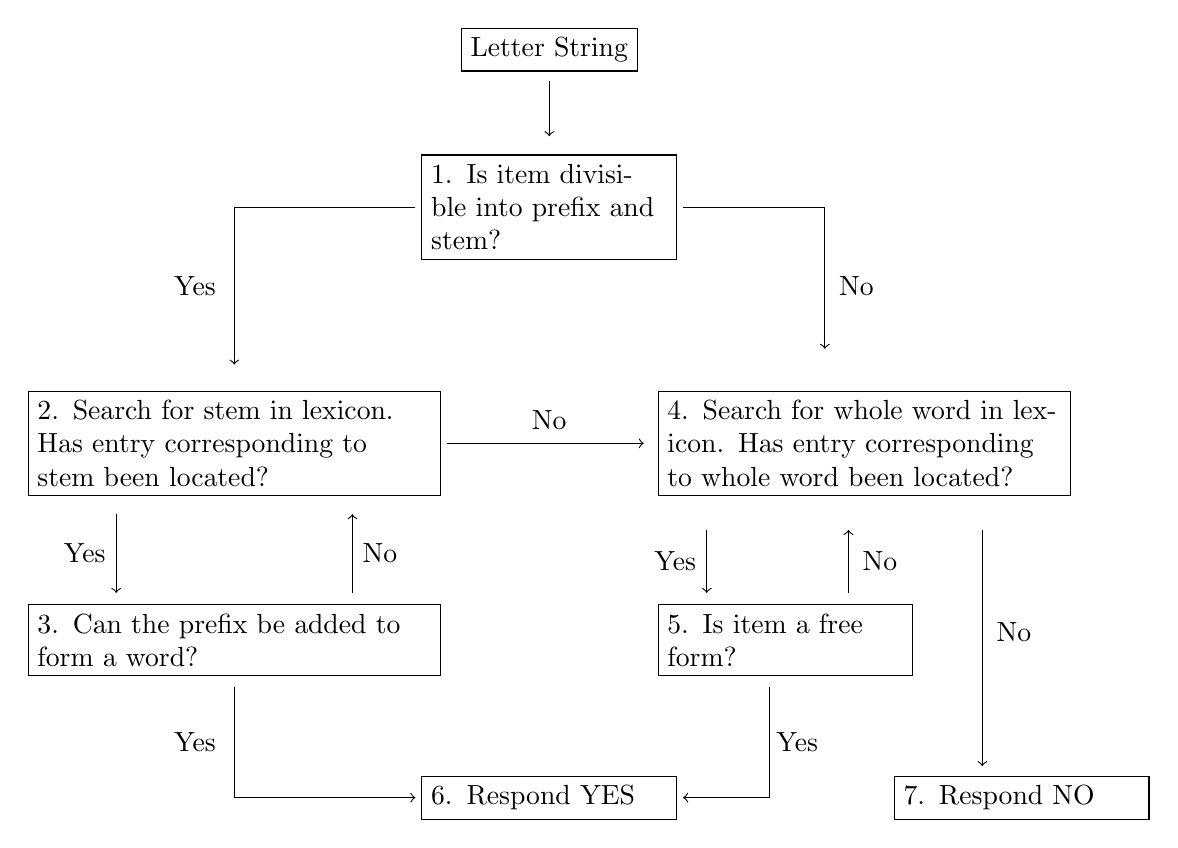
\begin{tikzpicture}%[scale=0.80]
\draw (5,8) node [shape= rectangle, draw] (signal) {Letter String};
\draw (5,6) node [text width=3cm, align=left, shape= rectangle,
draw] (first) {1. Is item divisible
  into prefix and stem?};
% \draw [->] (signal) -- (first);
\draw [->] (5,7.6) -- (5,6.9);
% Third row
\draw (1,3) node [text width=5cm, align=left, shape= rectangle,
draw] (second) {2. Search for stem in lexicon. Has entry corresponding
  to stem been located?};
\draw (9,3) node [text width=5cm, align=left, shape= rectangle,
draw] (fourth) {4. Search for whole word in lexicon. Has entry
  corresponding to whole word been located?};
\draw [-] (1,6) -- (3.3,6);
\draw [->] (1,6) -- (1,4);
% \draw [->] (first) -- (second);
% \draw [->] (first) -- (fourth);
\draw [-] (6.7,6) -- (8.5,6);
\draw [->] (8.5,6) -- (8.5,4.2);
\draw (8.9,5) node {No};
\draw (.5,5) node {Yes};
% \draw [->] (second) -- (fourth);
\draw [->] (3.7,3) -- (6.2,3);
\draw (5,3.3) node {No};

% Fourth row
\draw (1,.5) node [text width=5cm, align=left, shape= rectangle,
draw] (third) {3. Can the prefix be added to form a word?};
\draw (8,.5) node [text width=3cm, align=left, shape= rectangle,
draw] (fifth) {5. Is item a free form?};
% \draw [->] (second) -- (third);
\draw [->] (7,1.9) -- (7,1.1);
\draw [<-] (8.8,1.9) -- (8.8,1.1);
\draw [->] (-.5,2.1) -- (-.5,1.1);
\draw [<-] (2.5,2.1) -- (2.5,1.1);

\draw [->] (10.5,1.9) -- (10.5,-1.1);

\draw (-.9,1.6) node {Yes};
\draw (2.85,1.6) node {No};
% Fifth row
\draw (5,-1.5) node [text width=3cm, align=left, shape= rectangle,
draw] (first) {6. Respond YES};
\draw (11,-1.5) node [text width=3cm, align=left, shape= rectangle,
draw] (first) {7. Respond NO};
\draw [-] (1,-0.1) -- (1,-1.5);
\draw [->] (1,-1.5) -- (3.3,-1.5);
\draw [<-] (6.7,-1.5) -- (7.8,-1.5);
\draw [-] (7.8,-1.5) -- (7.8,-0.1);
\draw (.5,-.8) node {Yes};
\draw (8.15,-.8) node {Yes};
\draw (10.9,.6) node {No};
\draw (9.2,1.5) node {No};
\draw (6.6,1.5) node {Yes};
% % \node (context) {};
% \node [shape= rectangle, draw] (intermediate) [below=of signal]  {intermediate access representation};

% \node [shape= rectangle, draw] (access-rep) [below=of intermediate]  {access representation};
% \node [shape= rectangle, draw] (concept-nodes) [below=of access-rep]  {concept nodes};
% % \node (placeholder) [below=of concept-nodes]  {};
% \node [shape= rectangle, draw] (synsem-rep) [below=of concept-nodes]  {syntactic
%   representations \hspace*{2cm}semantic representations};
% % \node (syn-rep) [left=of placeholder]  {syntactic representations};
% % \node (sem-rep) [right=of placeholder]  {semantic representations};
% \node [shape= circle, draw] (output) [below=of synsem-rep]  {output};

% \draw [->] (signal) -- (intermediate);
% \draw [->] (intermediate) -- (access-rep);
% \draw [<->] (access-rep) -- (concept-nodes);
% \draw [<->] (concept-nodes) -- (synsem-rep);
% \draw [->] (synsem-rep) -- (output);

% \draw (-6.0,-4.9) rectangle (6,-1.6);
% \draw (-6.0,-8.7) rectangle (6,-5.4);

% \draw (-4.5,-2.15) node [text width=3cm, align=center] {segmentation and phonology}; 
% \draw (-4.5,-6.2) node [text width=3cm, align=center] {licensing and computation}; 

\end{tikzpicture}  
}

  \caption{Model for word recognition \citep{TaftandForster:1975}}
  \label{fig:taft_forster_word-recognition-model}
\end{center}
\end{figure}
\noindent
This model comes with 2 important features. First, it assumes that
morphological decomposition takes place in word recognition, the
relevant unit for the decomposition being the morpheme-level. Second,
it assumes that, for a specific string, only one specific
route is taken. That is, if a word is morphologically complex, it takes
the decompositional route, but if it is a simplex word, it takes the
whole-word route. 
While there have been many different responses to
their model, including e.g. \citet{ManelisandTharp:1977}, who rejected the very idea of
morphological decomposition in favor of whole-word look-up, the general
trend was soon towards mixed
models, that is, models that allow morphological decomposition and
whole-word look-up for the same items. An early example is the mixed model proposed in
\citet{Stannersetal:1979}, where one and the
same form can not only be stored in memory as a whole but can also at
least partially be
activated via a decompositional pathway.
\is{morphological decomposition|)}

% \citet{Stannersetal:1979}
% Using repetition priming combined with a lexical
% decision task, they investigated the English inflectional affixes \emph{-s},
% \emph{-ed} and \emph{-ing}, irregular past tense forms, and adjectival and
% nominal derivatives of verbs (e.g. \emph{selective/select} or
% \emph{appearance/appear}). In the interpretation of their findings, they argue
% that one plausible explanation lies in assuming that for regular inflection,
% the base form is accessed in memory, and the inflected form itself is not
% listed in memory, while in the other cases, the irregular or derived forms are
% stored in the lexical memory, but the verbal base is nevertheless partially
% activated, due to the interconnectness of the entries in the lexicon. 

% These early models did not focus on the role of semantic
% transparency. 
% However, semantic transparency plays a very important role in

A hugely influential and widely-cited model is the meta model for
morphological processing introduced in \citet{SchreuderandBaayen:1995}. This model is of additional interest, as it explicitly addresses problems relating to semantic transparency.
A schematic outline of this model, their
Figure 1, is reproduced in \figref{fig:schreuder_baayen_meta-model}.

% \resizebox{12cm}{!}{%
% \scalebox{.75}{%
\begin{figure}[h]
\begin{center}
\begin{tikzpicture}[>=stealth]
\node [shape= circle, draw] (signal) {speech signal};
% \node (context) {};
\node [shape= rectangle, draw] (intermediate) [below=of signal]  {intermediate access representation};

\node [shape= rectangle, draw] (access-rep) [below=of intermediate]  {access representation};
\node [shape= rectangle, draw] (concept-nodes) [below=of access-rep]  {concept nodes};
% \node (placeholder) [below=of concept-nodes]  {};
\node [shape= rectangle, draw] (synsem-rep) [below=of concept-nodes]  {syntactic
  representations \hspace*{2cm}semantic representations};
% \node (syn-rep) [left=of placeholder]  {syntactic representations};
% \node (sem-rep) [right=of placeholder]  {semantic representations};
\node [shape= circle, draw] (output) [below=of synsem-rep]  {output};

\draw [->,thick] (signal) -- (intermediate);
\draw [->,thick] (intermediate) -- (access-rep);
\draw [<->,thick] (access-rep) -- (concept-nodes);
\draw [<->,thick] (concept-nodes) -- (synsem-rep);
\draw [->,thick] (synsem-rep) -- (output);

\draw (-6.0,-4.9) rectangle (6,-1.6);
\draw (-6.0,-8.2) rectangle (6,-5.1);

\draw (-4.5,-2.25) node [text width=3cm, align=center] {segmentation and phonology}; 
\draw (-4.5,-5.8) node [text width=3cm, align=center] {licensing and computation}; 

\end{tikzpicture}  

  \caption{Meta model for morphological processing \citep{SchreuderandBaayen:1995}}
  \label{fig:schreuder_baayen_meta-model}
\end{center}
\end{figure}

\noindent
\citet{SchreuderandBaayen:1995} distinguish 3 stages:
segmentation, licensing, and combination. At the segmentation stage,
the speech input is mapped to access representations which are form-based representations of the speech signal. This is a 2-step
process, involving an intermediate access representation and, after segmentation, an access
representation proper. An
intermediate access representation might still contain more than one word,
whereas the access representation proper can at most correspond to one
complex word: ``Such `lexical' access
representations may be present for full complex forms, for stems,
whether bound or free, for affixes, and for clitics. They contain
modality-specific form information that is normalized both with
respect to the inherent variability in the speech signal and with
respect to the variability caused by phonological processes such as
vowel harmony and various kinds of assimilation
processes" \citep[133--134]{SchreuderandBaayen:1995}. 
The next 2 stages, licensing and computation, both take
place at the level of lexical representations. Lexical representations constitute the final output of the
lexicon. A lexical representation consists of a concept node,
which in turn is connected with syntactic and semantic
representations. The interplay between the concept nodes and these
syntactic and semantic representations constitutes one of the most
interesting aspects of the model. The concept node itself can be
understood as a bundling of links to specific syntactic and semantic
representations; concept nodes exist only for those concepts that
``receive verbal expression in the language at the form level"
\citep[136]{SchreuderandBaayen:1995}. That is, in this account,
lexical gaps like the missing liquid related counterpart to German \emph{satt} `full with respect to
food' don't have a concept node, though expressing a concept. Syntactic representations contain information on, among others,
subcategorization, word class, and argument structure.
\citet[136]{SchreuderandBaayen:1995} remain vague with respect to the
semantic representation (``specify various meaning aspects"). However,
in their figures and discussion it becomes clear that these various meaning aspects
are essentially what is responsible for the meaning of and meaning
differentiations between concept nodes. Semantic information is only
stored once, ``the links with the concept nodes serving as the
means for distinguishing and addressing concepts" \citep[140]{SchreuderandBaayen:1995}. 
\il{Dutch!{illustrating the Schroeder/Baayen model}|(}
Thus, the difference between Dutch
\emph{ruim} `spacious' and \emph{ruim-te} `space' is a difference in
the corresponding links to the syntactic and semantic representations,
which for \emph{ruim-te} include links to the syntactic node
NOUN, and to the semantic nodes ABSTRACT PROPERTY and SPACIOUSNESS,
cf. \citet[138]{SchreuderandBaayen:1995}.
 The link structure in this
model can be used to represent different degrees of semantic
transparency. This will become clearer when looking at how a novel
complex form leads to the generation of new lexical representations.

% In the case of monomorphemic words, the lexical
% representation is simply the concept node connected with the
% corresponding access representation, along with the concept's node
% associated syntactic and semantic representations. No licencing and
% composition is required in this case. 

% However, for novel complex
% forms, this mechanism ensures the generation of new lexical
% representations. 

How does the model deal with new complex combinations? Initially, at least 2
different access representations are activated, in turn leading to the
activation of the corresponding concept nodes. At this point, a
licensing mechanism checks whether the associated syntactic
presentations allow the system to proceed with meaning computation. In
particular, \citet[137]{SchreuderandBaayen:1995} distinguish 3
scenarios:
\begin{enumerate}
\item No new concept node is added if the meaning of a complex word
  can be obtained by the union of the relevant sets of
  representations. They exemplify this via Dutch plural formation by
  the regular plural \emph{-en} (e.g. \emph{boek} `book' $\rightarrow$ \emph{boek-en} `books').
\item A new concept node is created in any other case that involves computation.
\item Not fully semantically transparent forms also receive their own
  concept node.
\end{enumerate}

\is{frequency!{effects in the Schroeder/Baayen model}|(}
Note that word forms such as Dutch \emph{boek-en} `books', being transparent and
computable via set union, might nevertheless develop their own access
representations. \linebreak[3]Whether or not this happens is solely
frequency driven. However, even with their own access representation,
they will not develop a  concept node as long as their semantics
remains unchanged, that is, transparent.
\il{Dutch!{illustrating the Schroeder/Baayen model}|)}

The Schreuder/Baayen model uses spreading activation; as indicated in \figref{fig:schreuder_baayen_meta-model} by the double-headed
arrows, all levels except the intermediate access representations can
receive activation feedback from higher levels.  As \citeauthor{SchreuderandBaayen:1995} point out, this architecture
can account for a number of well-known frequency effects.
Word-frequency effects, for example, lead to higher activation levels of the
access representations, while the cumulative stem frequency effect is
best viewed as being due to heightened activation levels of the concept
node corresponding to the stem \citep[147]{SchreuderandBaayen:1995}. % cf. p. 147
\is{frequency!{effects in the Schroeder/Baayen model}|)}

\is{semantic transparency!{in the Schroeder/Baayen model}|(}
With regard to semantic transparency, \citet[140]{SchreuderandBaayen:1995} assume that ``a
semantically transparent relation between a complex word and its
constituents can be modeled as a substantial overlap between the set
of (semantic) representations of the complex word and the sets of
representations of its constituents".  In particular, empirical
effects of semantic transparency can be modeled via the flow of
activation (1)  between the concept nodes and the syntactic and
semantic nodes and (2) from the concept nodes to the access representations.

\il{Dutch!{illustrating the Schroeder/Baayen model}|(}
\citeauthor{SchreuderandBaayen:1995} illustrate the feedback to the concept
nodes with the help of the semi-transparent derivation \emph{groen-te} 
`vegetable' from \emph{groen} `green' and the abstract-noun forming
suffix \emph{te} and the fully transparent derivation \emph{trots-heid}
`pride', from \emph{trots} `proud/pride' and \emph{-heid}. For the
former, \citet[142]{SchreuderandBaayen:1995} assume that there is
hardly any activation from the semantic node of \emph{groente} to that
of \emph{groen}, since there are hardly any links between the concept
node of \emph{groente} and the semantic and syntactic nodes linked to
\emph{groen}. In contrast, for the latter, \emph{trotsheid}, both the concept node for
\emph{trots} as well as the one for \emph{-heid} will receive
activation feedback via the semantic representations shared with the
concept node of \emph{trotsheid}.  
\il{Dutch!{illustrating the Schroeder/Baayen model}|)}

The activation feedback from concept nodes to access representations is
proportional to the activation level of the concept nodes involved
\citep[142]{SchreuderandBaayen:1995}. That is, while for a
semantically transparent formation the highest extent of activation
feedback will flow from the concept node of the complex form itself to
its access representation, there will also be feedback from the
co-activated concept nodes to their respective access
representations. In contrast, for semantically opaque formations,
there will be little if any feedback to the individual constituents'
access representations, as the corresponding concept nodes are not
highly activated.

In addition, semantic transparency 
is hypothesized by \citet[146]{SchreuderandBaayen:1995} to also play a
role in the development of concept nodes for derivational
affixes. They predict an
earlier acquisition of transparent affixes, and they predict
the development of representations for bound stems only if these
participate in word formations that are compositional. % p. 147
% lexical representations 
\is{semantic transparency!{in the Schroeder/Baayen model}|)}

While \citet{SchreuderandBaayen:1995} are mainly concerned with
inflection and derivation, we can easily apply the model's general logic to
compounds. Thus, using \emph{bank barn} as an example of a novel
compound, the intermediate access representation % \emph{bank barn}, 
\textipa{[""b\ae NkbA:n]}
leads to the activation of the access representations for \emph{bank} and
\emph{barn}. These, in turn, lead to the activation of at least the
concepts BANK1 `institution that lends money etc.' and BANK2 `raised mass of earth', and BARN `farm outbuilding'. 
Based on the syntactic representations associated with the concept
nodes, meaning computation is licensed, since noun noun compounding is a 
 valid morphological operation in English. While it is partly the aim
of this work to find out how or to what extent one can compute a meaning
for these 2 items, it is clear that the computation involved will be
more than a simple set union. In fact, it seems a fair claim that all
compound formation surpasses a regular plural affix in complexity and
is typically more than just set union (recall that even the most
straightforward noun noun combination given in the introduction,
\emph{silk fabric}, already allows a construal with the \textsc{made of} relation). In consequence, this means that
after meaning computation, a new concept node BANK BARN will have come
into existence.

% The reasoning behind this model is best understood by first looking at a
% concrete example and then stepping through further features of the
% model. Thus, figure \ref{fig:cannibalizable} illustrates the processing of \emph{cannibalizable}.


    
  
% % \resizebox{12cm}{!}{%
% \scalebox{.80}{%
% \begin{figure}[h]
%   \begin{center}
% \begin{tikzpicture}
% \node [shape= circle, draw] (signal) {speech signal};
% % \node (context) {};
% \node [shape= rectangle, draw] (intermediate) [below=of signal]  {\textipa{""k\ae nIb@"laIz@bl}};
% \node (access-placeholder) [below=of intermediate]
% {};

% \node [shape= rectangle, draw] (access-rep-left) [left=of access-placeholder]
% {\textipa{"k\ae nIb@laIz}};
% \node [shape= rectangle, draw] (access-rep-right) [right=of access-placeholder]
% {\textipa{@bl}};


% \node [shape= rectangle, draw] (concept-node-left) [below=of access-rep-left]  {CANNIBALIZE};
% \node [shape= rectangle, draw] (concept-node-right) [below=of access-rep-right]  {ABLE};

% \node (concept-nodes-place) [below=of access-placeholder]  {};

% \node (synsem-rep-place) [below=of concept-nodes-place]  {};
% \node [shape= rectangle, draw] (synsem-rep-left) [below=of concept-node-left]  {syn/sem};

% \node [shape= rectangle, draw] (synsem-rep-right) [below=of concept-node-right]  {syn/sem};


% % \node (syn-rep) [left=of placeholder]  {syntactic representations};
% % \node (sem-rep) [right=of placeholder]  {semantic representations};
% \node [shape= circle, draw] (output) [below=2cm of synsem-rep-place]  {output};
% % \draw (0,-9) \node [shape= circle, draw] {output};

% \draw [->] (signal) -- (intermediate);
% % \draw [->] (intermediate) -- (access-rep);
% \draw [->] (intermediate) -- (access-rep-left);
% \draw [->] (intermediate) -- (access-rep-right);
% \draw [<->] (access-rep-left) -- (concept-node-left);
% \draw [<->] (access-rep-right) -- (concept-node-right);
% \draw [<->] (concept-node-left) -- (synsem-rep-left);
% \draw [<->] (concept-node-right) -- (synsem-rep-right);
% \draw [->] (synsem-rep-left) -- (output);
% \draw [->] (synsem-rep-right) -- (output);

% \draw (-6.0,-4.7) rectangle (6,-1.6);
% \draw (-6.0,-8.5) rectangle (6,-5.1);

% \draw (-4.5,-2.15) node [text width=3cm, align=center] {segmentation and phonology}; 
% \draw (-4.5,-7.7) node [text width=3cm, align=center] {licensing and computation}; 

% \end{tikzpicture}  
% \end{center}
% \label{fig:cannibalizable}
% \end{figure}
% In a first step, the speech signal is represented as an intermediate access
% represenation. Assuming for \emph{cannalizable} that it is a string
% encountered for the first time, but prosodically clearly recognizable as one
% rather low-level unit, the whole word constitutes the intermediate access
% representation. This representation, in turn, can be mapped onto two different
% access representation, standing for the base and the suffix,
% respectively. Both access representations are connected to their corresponding
% lexical representations, consisting of a concept node linked to its semantic
% and syntactic representation. It is now the work of the licensing and
% composition component to combine these two lexical representations and output
% a new lexical representation for the complex formation \emph{cannalizable}.


% I will come back to their model after discussing the psycholinguistic studies
% on the role of semantic transparency in compound processing.

% \fbox{
% \begin{minipage}{1.0\linewidth}
% \textbf{WOHIN DAMIT?}
%  As can be seen from the examples discussed above, complex nominals or, as the
% research was focussed on words, compounds, played no role in
% the development of these early models. However, compounds as a class seem to lend
% themselves further for investigation, especially when it comes to mixed
% models. Indeed, the high productivity of compound formation on the one hand
% and the high degree of opaqueness seen in compounds like \emph{buttercup}
% already make either of the first to models implausible. Manupilating a
% string's semantic transparency can then be used to get to a better
% understanding of the architecture of mixed models. 
 
% \end{minipage}
% }

% The role of compounds in model building


\citet{Libben:1998} introduces a model explicitly designed for
compounds, which in many aspects can be seen as building on the Schreuder/Baayen model. 
% \citet[33]{Libben:1998} argues that the Schreuder/Baayen model cannot easily handle
% assymmetries in the overlap of compounds and their constituents at the semantic level. We will come back to this point after presenting his model.  \textbf{WHY? COME BACK TO THIS POINT LATER}. 
\citet{Libben:1998}
distinguishes 3 levels: the stimulus level, the lexical
level, and the conceptual level.

The stimulus level is the level where morphological parsing takes
place. A left to right recursive parsing
  procedure checks both constituents for lexical status and thus
  avoids wrongly identifying a simplex word as a
  compound, e.g. dividing \emph{boycott} into \emph{boy} + \emph{cott}, while correctly identifying novel compounds, e.g. Libben's example
  \emph{redberry} (cf. \citealt{Libben:1994}, where he discusses a parser with these properties in detail).


Word forms, that is, stored representations of actual words, are represented at the lexical level. Libben illustrates
this level with the help of the existing
compounds \emph{strawberry} and \emph{blueberry}, the novel compound
\emph{redberry}, and the surname \emph{Thornberry}. \emph{Strawberry},
\emph{blueberry} and \emph{Thornberry} have representations at the
lexical level. In addition, the representations of
\emph{strawberry} and \emph{blueberry} have a structured
representation indicating their constituent
structure. In both cases, their 2 constituents are linked to
their respective lexical representations. In contrast, \emph{Thornberry} does
not have a structured representation and, consequentially, does not
contain links from \emph{thorn} and \emph{berry} to the respective
lexical entries. \emph{Redberry} does not have a representation at this level, as it is a new compound. 

\is{semantic transparency!{of constituents in Libben's model}|(}
The meanings are represented at the conceptual level. The links
between the lexical level and the conceptual level are used to model
constituent transparency. These links allow one to differentiate between
the \emph{straw} in \emph{strawberry} and the \emph{blue} in
\emph{blueberry}, both of which are linked to the respective
constituents at the lexical level, while only \emph{blue} is linked to
the corresponding entry at the conceptual level, too. Libben
distinguishes 8 different possible
configurations, with the first major distinction between componential
and noncomponential compounds. Componential compounds are endocentric
compounds. They can be paraphrased with the help of the pattern
`compound (noun 1 and noun 2/N1N2) is noun 2/N2', e.g. `a blueberry is a berry'. 
Noncomponential compounds do not allow this paraphrase (capturing
 the exocentric/bahuvrihi types in other classifications,
 cf. \citealt[Footnote 1]{Libben:1998}). Within both classes, Libben assumes a
 fourfold differentiation driven by constituent transparency: In the
 first configuration, transparent-transparent (TT), 
 both constituents are transparently related to the compound
 meaning. In the second configuration, transparent-opaque (TO), only the first constituent is
 transparent, whereas the second constituent is opaque. The third configuration, opaque-transparent (OT), shows the exact opposite arrangement: the first constituent is opaque and the second constituent is transparent. Finally, in the fourth configuration, both constituents are
 opaque, yielding opaque-opaque (OO) combinations. Libben's example for a
 componential TT compound is \emph{blueberry}. The componential TO and OT types are exemplified by \emph{shoehorn}
 and \emph{strawberry} respectively: The
 meaning of \emph{shoehorn}, `implement to be inserted at the heel of
 the shoe to ease the foot in', is not related to the meaning of
 \emph{horn}. Likewise, the meaning of \emph{strawberry} is not related to the meaning of
 \emph{straw}. Libben exemplifies the
 same 3 types for the noncomponential class, i.e., the
 non-endocentric compounds, with
 \emph{bighorn}, \emph{jailbird}, and \emph{yellow belly},
 respectively. A \emph{bighorn} is not a kind of horn, but a species
 of sheep with big horns. It is therefore noncomponential, but it is
 TT as the horns that are metonymically used to refer to the whole
 species are horns and are big. A \emph{jailbird} is no bird, but a
 person who is often or has been often in jail, therefore the first
 element is transparent. And a \emph{yellowbelly} is a coward, if,
 as Libben assumes, it is a noncomponential type OT, then he must have
 a paraphrase along the lines of `somebody with a bad or unsecure feeling in her
 belly' in his mind. 
% might be many
%  things, but what Libben must have had in mind for the TO
%  classification is probably one of its uses as an animal name, e.g.,
%  as the name for the yellow-bellied slider, a type of turtle, which
%  has yellow stripes, but not a yellow belly. 
% is a coward\texttt{[informal: a coward]}    

\citet{Libben:1998} does not give any examples for OO types in this
article. \citet{Libbenetal:2003} uses \emph{hogwash} `nonsense' to
exemplify the OO category. Conceptually, it is hard to see how one would
distinguish between componential and noncomponential types of OO
compounds from a
synchronic vantage point: if semantically neither constituent is
related to the compound meaning, the differentiation between
componential and noncomponential compounds becomes useless, even
though historically one could perhaps argue for componential vs.
noncomponential pathways of meaning development.

\enlargethispage{3\baselineskip}
Figures \ref{fig:libben-1998-TT-comp}--\ref{fig:libben-1998-OT-non}
reproduce his representation for the 3 non-OO types in the
noncomponential and componential versions, containing the links between and
within levels, cf. Figure 3, \citet[38]{Libben:1998}.
\pagebreak
% \vspace*{1cm}

% The following figures are set side by side using minipages inside a tabularx environment
% Every 2 figures are set in their own tabularx. The captions lead to overfull hboxes, probably due to scaling issues.
%
% \hspace*{-1.5cm}
% \begin{tabular}[!htb]{p{7cm}@{\hspace{.3cm}}p{7cm}}
% \noindent
% \begin{tabularx}{1\textwidth}{|X|X|}
% what&what\\
% \end{tabularx}
\noindent
\begin{tabularx}{1\textwidth}{XX}
%\fbox{
\begin{minipage}[t]{5.4cm}
% \begin{center}
% \hspace*{-1cm}
\resizebox{5.4cm}{!}{%
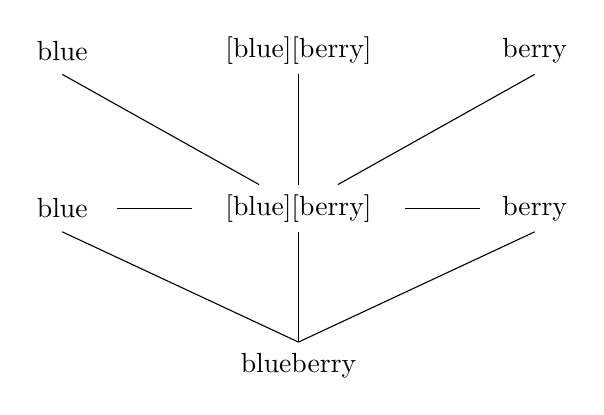
\begin{tikzpicture}
\draw (0,4) node [align=center] {[blue][berry]}; 
\draw (-3,4) node [align=center] {blue}; 
\draw (3,4) node [align=center] {berry}; 

\draw (0,2) node [align=center] {[blue][berry]}; 
\draw (-3,2) node [align=center] {blue}; 
\draw (3,2) node [align=center] {berry}; 

\draw (0,0) node [align=center] {blueberry}; 

\draw [-] (0,0.3) to  (0,1.7);
\draw [-] (0,0.3) to  (3,1.7);
\draw [-] (0,0.3) to  (-3,1.7);

\draw [-] (1.35,2) to  (2.3,2);
\draw [-] (-1.35,2) to  (-2.3,2);

\draw [-] (0,2.3) to  (0,3.7);
\draw [-] (0.5,2.3) to  (3,3.7);
\draw [-] (-0.5,2.3) to  (-3,3.7);
\end{tikzpicture}  
}
\captionsetup{font=small,justification=raggedright,singlelinecheck=on}
\captionof{figure}{TT componential}
%  \caption{Libben (1998): Constituency and componentiality at the lexical and conceptual levels}
  \label{fig:libben-1998-TT-comp}
% \end{center}
% \end{figure}
  
\end{minipage}%}
&
%\fbox{
\begin{minipage}[t]{5.4cm}
% \begin{figure}[h]
% \begin{figure}
% \begin{center}
% \hspace*{-1cm}
\resizebox{5.4cm}{!}{%
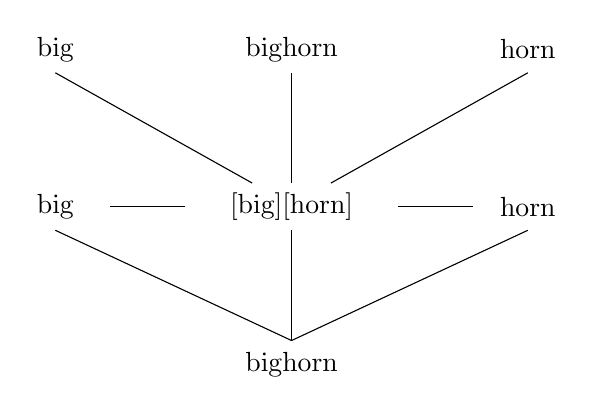
\begin{tikzpicture}
\draw (0,4) node [align=center] {bighorn}; 
\draw (-3,4) node [align=center] {big}; 
\draw (3,4) node [align=center] {horn}; 

\draw (0,2) node [align=center] {[big][horn]}; 
\draw (-3,2) node [align=center] {big}; 
\draw (3,2) node [align=center] {horn}; 

\draw (0,0) node [align=center] {bighorn}; 

\draw [-] (0,0.3) to  (0,1.7);
\draw [-] (0,0.3) to  (3,1.7);
\draw [-] (0,0.3) to  (-3,1.7);

\draw [-] (1.35,2) to  (2.3,2);
\draw [-] (-1.35,2) to  (-2.3,2);

\draw [-] (0,2.3) to  (0,3.7);
\draw [-] (0.5,2.3) to  (3,3.7);
\draw [-] (-0.5,2.3) to  (-3,3.7);


\end{tikzpicture}  
}
\captionsetup{font=small,justification=raggedright,singlelinecheck=on}
\captionof{figure}{TT noncomponential}
%  \caption{Libben (1998): Constituency and componentiality at the lexical and conceptual levels}
  \label{fig:libben-1998}
% \end{center}
% \end{figure}
  
\end{minipage}
%}
% \end{tabular}
\end{tabularx}
\vspace*{1cm}

\noindent
\begin{tabularx}{1\textwidth}{XX}
%\fbox{
\begin{minipage}[t]{5.4cm}
\resizebox{5.4cm}{!}{%
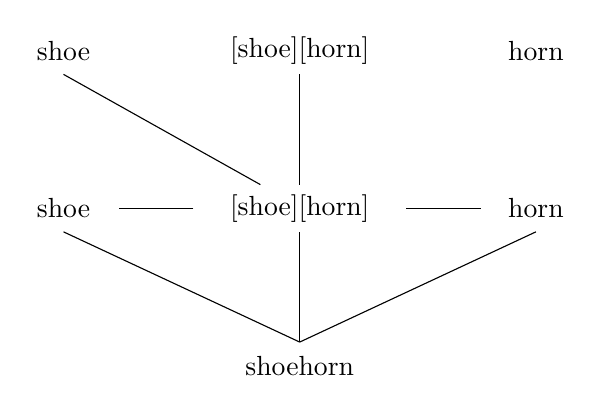
\begin{tikzpicture}
\draw (0,4) node [align=center] {[shoe][horn]}; 
\draw (-3,4) node [align=center] {shoe}; 
\draw (3,4) node [align=center] {horn}; 

\draw (0,2) node [align=center] {[shoe][horn]}; 
\draw (-3,2) node [align=center] {shoe}; 
\draw (3,2) node [align=center] {horn}; 

\draw (0,0) node [align=center] {shoehorn}; 

\draw [-] (0,0.3) to  (0,1.7);
\draw [-] (0,0.3) to  (3,1.7);
\draw [-] (0,0.3) to  (-3,1.7);

\draw [-] (1.35,2) to  (2.3,2);
\draw [-] (-1.35,2) to  (-2.3,2);

\draw [-] (0,2.3) to  (0,3.7);
% \draw [-] (0,2.3) to  (3,3.7);
\draw [-] (-0.5,2.3) to  (-3,3.7);


\end{tikzpicture}  
}
\captionsetup{font=small,justification=raggedright,singlelinecheck=on}
\captionof{figure}{TO componential}
%  \caption{Libben (1998): Constituency and componentiality at the lexical and conceptual levels}
  \label{fig:libben-1998}
\end{minipage}
% }
&
\begin{minipage}[t]{5.4cm}
\resizebox{5.4cm}{!}{%
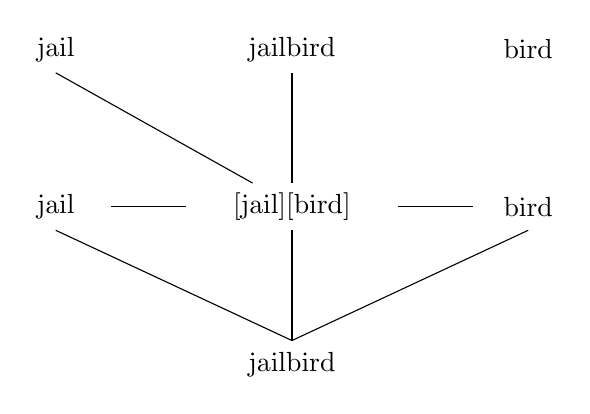
\begin{tikzpicture}
\draw (0,4) node [align=center] {jailbird}; 
\draw (-3,4) node [align=center] {jail}; 
\draw (3,4) node [align=center] {bird}; 

\draw (0,2) node [align=center] {[jail][bird]}; 
\draw (-3,2) node [align=center] {jail}; 
\draw (3,2) node [align=center] {bird}; 

\draw (0,0) node [align=center] {jailbird}; 

\draw [-] (0,0.3) to  (0,1.7);
\draw [-] (0,0.3) to  (3,1.7);
\draw [-] (0,0.3) to  (-3,1.7);

\draw [-] (1.35,2) to  (2.3,2);
\draw [-] (-1.35,2) to  (-2.3,2);

\draw [-] (0,2.3) to  (0,3.7);
% \draw [-] (0,2.3) to  (3,3.7);
\draw [-] (-0.5,2.3) to  (-3,3.7);


\end{tikzpicture}  
}
\captionsetup{font=small,justification=raggedright,singlelinecheck=on}
\captionof{figure}{TO noncomponential}
%  \caption{Libben (1998): Constituency and componentiality at the lexical and conceptual levels}
  \label{fig:libben-1998_TOnoncomponential}
\end{minipage}
\end{tabularx}
\vspace*{1cm}

% \hspace*{-1.5cm}
\noindent
\begin{tabularx}{1\textwidth}{XX}
\begin{minipage}[t]{5.4cm}
\resizebox{5.4cm}{!}{%
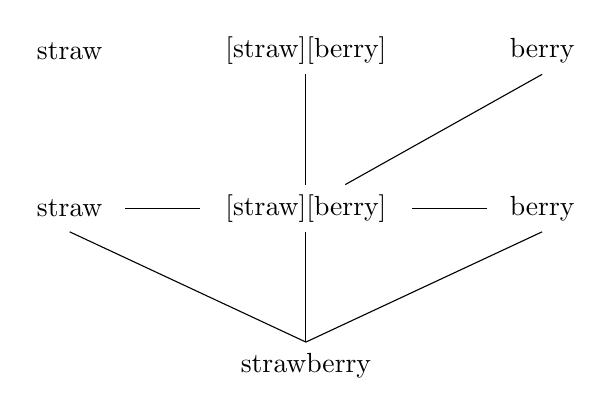
\begin{tikzpicture}
\draw (0,4) node [align=center] {[straw][berry]}; 
\draw (-3,4) node [align=center] {straw}; 
\draw (3,4) node [align=center] {berry}; 

\draw (0,2) node [align=center] {[straw][berry]}; 
\draw (-3,2) node [align=center] {straw}; 
\draw (3,2) node [align=center] {berry}; 

\draw (0,0) node [align=center] {strawberry}; 

\draw [-] (0,0.3) to  (0,1.7);
\draw [-] (0,0.3) to  (3,1.7);
\draw [-] (0,0.3) to  (-3,1.7);

\draw [-] (1.35,2) to  (2.3,2);
\draw [-] (-1.35,2) to  (-2.3,2);

\draw [-] (0,2.3) to  (0,3.7);
\draw [-] (0.5,2.3) to  (3,3.7);
% \draw [-] (0,2.3) to  (-3,3.7);


\end{tikzpicture}  
}
\captionsetup{font=small,justification=raggedright,singlelinecheck=on}
\captionof{figure}{OT componential}
%  \caption{Libben (1998): Constituency and componentiality at the lexical and conceptual levels}
  \label{fig:libben-1998}
\end{minipage}
&
\begin{minipage}[t]{5.4cm}
\resizebox{5.4cm}{!}{%
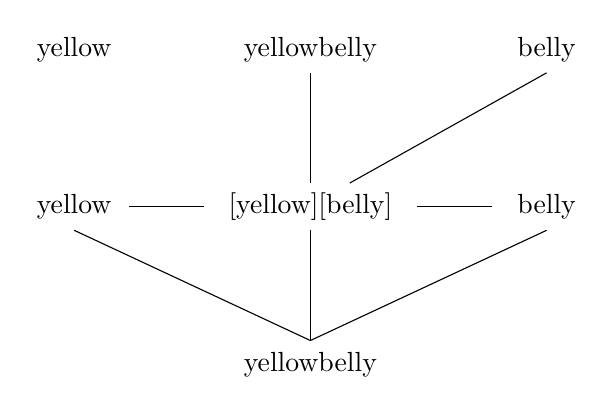
\begin{tikzpicture}
\draw (0,4) node [align=center] {yellowbelly}; 
\draw (-3,4) node [align=center] {yellow}; 
\draw (3,4) node [align=center] {belly}; 

\draw (0,2) node [align=center] {[yellow][belly]}; 
\draw (-3,2) node [align=center] {yellow}; 
\draw (3,2) node [align=center] {belly}; 

\draw (0,0) node [align=center] {yellowbelly}; 

\draw [-] (0,0.3) to  (0,1.7);
\draw [-] (0,0.3) to  (3,1.7);
\draw [-] (0,0.3) to  (-3,1.7);

\draw [-] (1.35,2) to  (2.3,2);
\draw [-] (-1.35,2) to  (-2.3,2);

\draw [-] (0,2.3) to  (0,3.7);
\draw [-] (0.5,2.3) to  (3,3.7);
% \draw [-] (0,2.3) to  (-3,3.7);


\end{tikzpicture}  
}
\captionsetup{font=small,justification=raggedright,singlelinecheck=on}
\captionof{figure}{OT noncomponential}
%  \caption{Libben (1998): Constituency and componentiality at the lexical and conceptual levels}
  \label{fig:libben-1998-OT-non}
\end{minipage}
\end{tabularx}
\vspace*{.5cm}


\noindent
The links within a level and between levels are always facillatory. The absence of links creates competition, leading to the eventual inhibition of non-targets.

% Comparison to the Schreuder-Baayen model
\citet[33]{Libben:1998} appears to endorse the operationalization of
semantic transparency proposed in
\citet[140]{SchreuderandBaayen:1995} (see above), that is, that
semantic transparency can be modeled as overlap between the semantic
representations of a complex word and the semantic representations of its
constituents. Furthermore, his stimulus level
corresponds to the level of access representations in the
Schreuder/Baayen model. It is in the higher levels that the 2 models
diverge, with Libben contending that the Schreuder/Baayen model does not ``easily
handle asymmetries in this overlap" \citep[33]{Libben:1998}.  He does
not clarify which asymmetries exactly he views as problematic. If one
considers his 3 examples for the componential types,
\emph{blueberry}, \emph{shoehorn}, and \emph{strawberry}, the core
difference between the 3 types of compounds lies in  the links
between lexical and conceptual level, with \emph{blueberry} linking to
both constituents' conceptual representation, whereas the other 2 compounds only
link to the respective transparent constituent's representation. On
the lexical level, they are alike insofar as their structured
representation is linked to the representations of the corresponding
constituents, in contrast to Libben's assumption for
\emph{Thornberry}. In the Schreuder/Baayen model, the 3 types
can be distinguished via their different connection strength to
semantic representations shared with the concept nodes of the
constituents, while their constituent structure is discernable
due to the interplay between access representations and concept
nodes. It is not clear to me how to best represent \emph{Thornberry}
in the Schreuder/Baayen model. However, as far as I can see, there is
also no empirical evidence to show that it behaves differently from,
e.g., OO compounds. All in all, while Libben's discussion is a helpful
clarification of the different types of compounds one can find, it
seems that his remark with regard to the observed asymmetry is of
greater relevance in distinguishing compound semantics from the
patterns found in derivation and inflection, but does not pose any
specific problem for the general structure of the Schreuder/Baayen model.
\is{models of morphological processing!{morpheme-based}|)}
\is{semantic transparency!{of constituents in Libben's model}|)}


% : ``An assumption crucial to the
% theory developed here is that a semantically transparent relation
% between complex word and its constituents can be modeled as a
% substantial overlap between the set of (semantic) representations of
% the complex word and the sets of representations of its
% constituents". However, he does This
% point will be discussed in detail in section \textbf{BLABLA}.



\subsection{Models without morphemes}
\label{sec:non-classical}
\is{models of morphological processing!{without morphemes}|(}
From the 1980s onward, alternative models of morphological
processing have been developed that differ radically from the
models discussed so far. Technically, the most important difference is
that morphemes are not represented as distinct
representational entities anywhere in these models. As far as their
empirical coverage is concerned, many
models, especially if they are actually implemented, model only very
specific aspects of morphological processing.  Most of the models
do  not target compounds in particular. Here, I present the main ideas
behind the very
influential models of \citet{RumelhartandMcClelland:1986} and
\citet{Bybee:1995} and then discuss in detail the amorphous model
proposed in \citet{Baayenetal:2011}, which addresses compound
processing as well as the issue of semantic transparency.

% Most of the discussion with regard to these models, however,
% has taken place against the background of inflection and derivational
% morphology, with one very prominent line of discussion being concerned
% mainly with the treatment of regular vs. irregular morphology. Here,
% non-classical models have been mainly argued against views from Pinker
% and colleagues, who, for the English regular and irregular past tense,
% argued for a symbolic rule for the regular cases and lexical
% representations for the irregular cases. These models are referred to
% in \citet[427]{Bybee:1995} as dual-processing models. \textbf{ADD Sources!}

%%%%%%%%%%%%%%%%%%%%%%%%%%%%%%%%%%%%%%%%%%%%%%%%%%%%%%%%%%%%%%%%%%%%%%%%
%%
%%            Rumelhart and McClelland
%%
%%%%%%%%%%%%%%%%%%%%%%%%%%%%%%%%%%%%%%%%%%%%%%%%%%%%%%%%%%%%%%%%%%%%%%%%

% \subsubsection{Rumelhart and McClelland 1986}
\subsubsection{Rumelhart and McClelland}
\label{sec:rumel}


\citet{RumelhartandMcClelland:1986} proposed a connectionist model in order to model the time course
of learning the past tense forms of English irregular and regular
verbs.
% \citet{RumelhartandMcClelland:1986} 
Their model is a response to views on
inflection in English that assume that part of acquiring morphology is
acquiring, or inducing, rules (they point to \citealt{Pinker:1984} as
an example of a model based on this view). English past tense formation is of
particular interest in this respect, because the regular
past tense formation via the addition of \emph{-ed} to the end of a
verb can be seen as a typical example of word form formation by rule. In consequence, the language learner will at one point have
learned this specific rule. In contrast, in their model, such a rule
is never explicitly stated anywhere, but the same behavior falls out
from properties of the model. % Note that in contrast to the models discussed before, this 
The model is
very restricted in its domain, since its goal is only to produce the
phonological representation of the past tense from the phonological
representations of the root form. However, this allows one to clearly
see which core aspects are important for this and similar
models. 
\figref{fig:RumelhartMcClelland}, their Figure 1, shows the basic structure of their model.
\begin{figure}[h]
  \centering
% Declare layers
\pgfdeclarelayer{background}
\pgfsetlayers{background,main}

\resizebox{\textwidth}{!}{%
% Styles
\tikzstyle{information text}=[text badly centered,font=\small,text width=3cm]
\begin{tikzpicture}[scale=.8,cap=round]
    % The graphic
    \begin{scope}[>=stealth', line width=1pt]
        \draw[->] (1,.9) node[below, information text]
            {Phonological representation of root form } -- (1,1.8);
        \draw[->] (5,-.2) node[below,information text]
            {Wickelfeature representation of root form } -- (5,.8);
        \draw[->] (11,-.2) node[below,information text]
            {Wickelfeature representation of past tense } -- (11,.8);
        \draw[->] (16,0.9) node[below,information text]
            {Phonological representation of past tense } -- (16,1.8);
    \end{scope}
    \draw (3,6) node[information text] { Fixed Encoding Network };
    \draw (8,6) node[information text, text width=4cm, ]
        { Pattern Associator Modifiable Connections };
    \draw (13.5,6) node[information text] { Decoding/Binding Network };
    % draw the nodes
    \foreach \x in {1,16}
        \foreach \y in {2,3,4} {
        \filldraw[fill=white] (\x,\y) circle (0.1);
        }
    \foreach \x in {5,11}
        \foreach \y in {1,2,3,4,5} {
            \filldraw[fill=white] (\x,\y) circle (0.1);
        }
    % The lines connecting the nodes are drawn in the background layer.
    % This way we can hide the lines behind the nodes and don't worry
    % about the width of each node.    
    \begin{pgfonlayer}{background}
        % we add the lines for the nodes starting in y 2,3, and 4
        \foreach \xa / \xb in {1 / 5, 5 / 11 , 11 / 5 , 16 / 11}
            \foreach \ya / \yb / \yc / \yd / \ye in {2 / 3 / 4 / 5 / 1, 
            3 / 4 / 5 / 1 / 2, 4 / 5 / 1 / 2 / 3} {
                \draw (\xa,\ya) -- (\xb,\ya);
                \draw (\xa,\ya) -- (\xb,\yb);
                \draw (\xa,\ya) -- (\xb,\yc);
                \draw (\xa,\ya) -- (\xb,\yd);
                \draw (\xa,\ya) -- (\xb,\ye);
            }
        % add remaining lines from y1 to y5
        \foreach \xa / \xb in {5 / 11 , 11 / 5}
            \foreach \ya / \yb in {1 / 5, 5 / 1} {
            \draw (\xa,\ya) -- (\xb,\ya);
            \draw (\xa,\ya) -- (\xb,\yb);
        }
    \end{pgfonlayer}
\end{tikzpicture}
}
% Author: Robert Felty
% Source: http://blog.robfelty.com/2007/02/14/pgf-gallery
% Model structure from Rumelhart \& McClelland (1986, p .222)%
% \textbf{MENTION SOMEWHERE THE SOURCE FOR THE CODE! -> acknowledgements}
%  http://www.texample.net/tikz/examples/about/
  \caption{A connectionist model for the English past tense \citep[222]{RumelhartandMcClelland:1986}. The \LaTeX {} code for the reproduction of their figure was written by Robert Felty and is available at \url{http://www.texample.net}.}
\label{fig:RumelhartMcClelland}
\end{figure}

Of particular interest are the levels of representation they assume,
the mechanism that links the levels, and the way the model learns. 
% I will discuss both of them in turn.
%As can be seen in figure \ref{fig:RumelhartMcClelland},
\citet{RumelhartandMcClelland:1986} distinguish
 4 different levels, 2 for the
phonological representations and 2 for so-called Wickelfeature
representations. These representations are paired, that is, there is a
phonological representation and a Wickelfeature representation of the
root form of an English
verb, and a phonological representation and a Wickelfeature
representation of the past tense of an English verb.
The Wickelfeature representations are  feature-based
representations of 3-phone
sequences, the Wickelphones, named by \citet{RumelhartandMcClelland:1986} after the proposal in 
\citet{Wickelgren:1969}.
% http://www.columbia.edu/~nvg1/Wickelgren/
The decoding and encoding networks are fixed, that is, there is no
variation in how the input phonemic representations are translated
into Wickelfeatures, nor is there variation in how the output Wickelfeature representations
are mapped on the output phonemic representations.

The core
of this model is the pattern associator which contains modifiable
connections between the input units,
that is, the Wickelfeature representations of the root forms, and the
output units, the Wickelfeature representations of the output
forms. Whether a unit is turned on or not depends on a probability
function which in turn depends on threshold values of the units and
the input they receive. Importantly, the units on the same level have
no interconnections and there is also no feedback in this
model. With this rather simple model architecture, many core
characteristics of learning the English past tense could be correctly modeled.

%%%%%%%%%%%%%%%%%%%%%%%%%%%%%%%%%%%%%%%%%%%%%%%%%%%%%%%%%%%%%%%%%%%%%%
%%
%%  BYBEE 1995 regular morphology and the lexicon
%%
%%%%%%%%%%%%%%%%%%%%%%%%%%%%%%%%%%%%%%%%%%%%%%%%%%%%%%%%%%%%%%%%%%%%%%

\subsubsection{Bybee's network model}
\label{sec:bybee}

Bybee's network model was originally proposed in \citet{Bybee:1985}
and \citet{Bybee:1988} (as \citealt[428]{Bybee:1995} points out, a model
with the same properties was proposed in \citealt{Langacker:1987} and \citealt{Langacker:1988}). Here, I follow her overview in
\citet[428--431]{Bybee:1995}. 

% \citet[428-431]{Bybee:1995} gives a summary of the core properties of her network model.
The network model is word-based, it can thus be seen as a lexicon
organized as a network. In this lexicon, words  have varying degrees of
lexical strength. The prime factor determining lexical strength is a word's token frequency. 
Words are related to other words via sets of
lexical connections between identical and similar phonological and
semantic features. While the words are not broken up into their
constituent morphemes, a morphological structure emerges due to the
intra-lexical connections. The lexical connections vary in
strength. Factors that influence connection strength are the type and
the number of shared features, and the token frequency of a specific
word. \is{frequency!{in Bybee's network model}|(}
% High-frequency words are easy to access,  serve as bases of
% morphological relations, 
Bybee argues that high frequency words  have greater lexical autonomy,
which is reflected in weaker
connections to other words. This idea is ``based on the common-sense
observation that items that are of high frequency in the input can be
learned on their own terms, while lower-frequency items are better
learned in relation to existing items" \citep[429]{Bybee:1995}. She further argues that phenomena such as suppletion and the known
resistance of high frequency irregulars to change are both linked to
lexical autonomy.
\is{frequency!{in Bybee's network model}|)}

Sets of words with similar patterns of semantic and phonological
connections reinforce each other, leading to emergent generalizations,
which are also refered to as schemata. Whether or not a schema is extended to other words
depends on the defining properties of the schema, e.g. whether it is
very general or very specific, and the strength of the schema,
which is derivable from the number of items that reinforce the
schema. \citet{Bybee:1995} distinguishes 2 types of schemas.
Source-oriented schemas generalize over pairs of basic and derived
forms. ``These correspond roughly to generative rules, since they can be
thought of as instructions for how to modify one form in order to
derive another" \citep[430]{Bybee:1995}. The regular past
tense formation in English with the suffix \emph{-ed} is captured by such a schema.

Product-oriented schemas, in contrast, are
generalizations over sets of complex/derived forms. Bybee exemplifies
this type of schema with the help of sub-regularities in English past
tense irregulars, e.g. the subclass containing \emph{strung, stung, flung, hung} etc. 
% this is Bybees example!
Membership in
these schemas, so Bybee,
is based on \isi{family resemblance}.

Bybee herself has not implemented her model; however, she 
states: ``Connectionist simulations could be thought of as testing
some of the properties of the network model and Langacker's cognitive
grammar, but the model itself is more complex and accounts for more
phenomena than any existing connectionist model''
\citep[428]{Bybee:1995}. Besides connectionist models, analogical
models come to mind as candidates for the implementation of the
product oriented schemas. Analogical models have been successfully used for some morphological phenomena (e.g. \citealt{Arndt-Lappe:2011} for stress assignments in English noun noun compounds or \citealt{Arndt-Lappe:2014} for the affix rivalry between English \emph{-ity} and \emph{-ness}).
%  AM algorithm, Skousen \& 
% Stanford, 2007)

\subsubsection{\citet{Baayenetal:2011}}
\label{sec:baayen2011}

\citet{Baayenetal:2011} present a very ambitious implemented
morphological model, the naive discriminative reader. It is of particular interest for my work, because
in some of the simulations run with the model, the issue of semantic
transparency is explicitly addressed. In contrast, the triangle model of
\citet{HarmandSeidenberg:2004}, aspects of which the naive
discriminative reader follows (cf. \citealt[439--440]{Baayenetal:2011}), does not address this
issue. Here, I aim at explaining its general structure, while
focusing on the place of semantic transparency in this model. 

The modeling target of Baayen et al's (2011) model are morphological effects in
visual comprehension, which they assess by using \isi{lexical decision} data.
% that is, as far as experimental effects are
% concerned, its scope is restricted to lexical decision.
% structure
It is a 2-layered symbolic network model, with unigrams and bigrams
as cues, and meanings as outcomes. Key to the model is the learning algorithm of
\citet{WagnerandRescorla:1972}. 
In \citet{Baayenetal:2011}, the modeling focuses on the end stage of the
lexical 
learning process: the cues, unigrams and bigrams, are already
associated with the outcomes, the meanings. These meanings range from word meanings
to inflectional and affixal meanings, that is, nominative case as well
as whatever a suffix such as \emph{-ness} stands for are meanings. Since the model has been
trained, it 
is in a state of equilibrium. 

Following \citeauthor{Baayenetal:2011}'s (\citeyear[450]{Baayenetal:2011}) representation, 
the association strength $V_{i}^{t + 1}$ from a cue $C_{i}$ at time
$t + 1$ results from its previous association strength $V_{i}^{t}$ plus the change in
association strength $\Delta V_{i}^{t}$. The change in association
strength is calculated according to the equation in \Next,
cf. \citet[450]{Baayenetal:2011}.\footnote{Note that I adjusted the
  index in the first if-statement to the index of the cue under
  discussion, $C_{i}$. This seems to be a mistake in the equation in
  \citet[450]{Baayenetal:2011}, cf. also equation (2) in
  \citet[299]{Baayen:2011}, where the index is set to the cue under discussion.}


\ex.  
\resizebox{.9\textwidth}{!}{%
$\Delta V_{i}^{t} =
\begin{cases}
  0 &\mbox{if ABSENT}(C_i,t)\\ % corrected after the equation in corpus linguistics and naive discriminative learning \citet[299]{Baayen:2011}
% \\
\alpha_i  \beta_1(\lambda -\Sigma_{\text{PRESENT}(C_j,t)}V_j) &\text{if
  PRESENT}(C_j,t) \;\&\; \mbox{PRESENT}(O,t)\\
\alpha_i, \beta_2(0 -\Sigma_{\text{PRESENT}(C_j,t)}V_j) &\text{if PRESENT}(C_j,t)\; \& \;\mbox{ABSENT}(O,t)\\
\end{cases}
$}\\\vspace*{.5em}
{}\\
% Calculating the change in association strength with the help of the
% Rescorla-Wagner equations; 
ABSENT/PRESENT: cue/outcome is absent or present;\\ standard settings for the parameters:
$\lambda$ = 1, all $\alpha$'s equal, $\beta_1$ = $\beta_2$
% checked, this is how it is


The first condition states that there is no change in association
strength from a cue $C_{i}$ to an outcome if the cue is absent. The
second and third conditions handle the changes in association strength
from cue $C_{i}$ to an outcome when the cue is present. If the cue
co-occurs with the outcome, the change in association strength is
positive and the cue's activation strength increases. If the cue
occurs, but the outcome is absent, its association strength decreases.

Both changes in activation strength depend on the number and
activation strength of other cues that are present. In particular, the higher
the summed activation levels of other cues present, the lower
the change in activation strength for cue $C_{i}$ if the outcome is present; if
the outcome is absent, the higher
the summed activation levels of other cues present, the higher the
negative change in activation strength for cue $C_{i}$.

\citet[450]{Baayenetal:2011} point out that at the end of its
learning, ``[t]he Rescorla-Wagner algorithm provides the
maximum-likelihood estimates of the weights on the connections between
letter unigrams and bigrams and word meanings."
To derive the association weights in the system in a stable state,
reaching an equilibrium, \citet{Baayenetal:2011} use a method
developed in \citet{Danks:2003}, who showed that solving the equation
in \Next, reproducing (9) in \citet{Baayenetal:2011}, allows one to derive the association strengths of the individual
cues.

\ex.
% \begin{equation*}
\( \displaystyle Pr(O|C_j) - \sum_{j=0}^{n}{Pr(C_j|C_i)V_j} = 0 \)  
% \end{equation*}
\\ $Pr(O|C_j)$ represents the conditional probability of the outcome
given cue C$_i$, and $Pr(C_j|C_i)$ the conditional probability of
cue C$_j$ given cue C$_i$. 

In order to solve this equation, \citet{Baayenetal:2011} for
simplicity's sake assume that the association strengths from letter
uni- and bigrams to meanings are modeled independently from all other
outcomes. They therefore refer to their model as a naive model, in
reference to the similarly simplifying assumption of conditional
independence for naive Bayes classifiers.

% Equilibrium training
In order to create a model in equilibrium, the authors proceeded as
follows:
\begin{enumerate}
\item They created a lexicon of 24,710 word types by selecting lexical
  items from \isi{CELEX} (cf. \citealt{Baayenetal:1995}) and from a number of
  individual psycholinguistic studies. All inflectional forms were
  also included.
\item The selected words were inserted into 13 different contexts and
  the resulting search patterns were used to extract a phrasal lexicon
  from the \isi{BNC}, consisting of 11,172,554 phrase tokens.
\item The connection weights for the Rescorla-Wagner network were
  calculated on the basis of this lexicon and the equilibrium equations.
\end{enumerate}
%   \frametitle{Equilibrium training}
%   \begin{itemize}
%   \item CELEX:
%     \begin{enumerate}
%     \item All monomorphemic nouns, verbs, adjectives 
%     \item All compounds/derived forms with items in 1. as base
%     \item All of these word's inflectional forms

%     \end{enumerate}

%   \item word stimuli from a number of studies
%   \item[$\rightarrow$] lexicon of 24710 word types
%   \item BNC:
%     \begin{itemize}
%     \item lexicon plugged into context: retrieved occurences plus preceding
%    words from BNC 
%     \item Resulting phrasal lexicon corresponding to quarter of corpus in
%   token size
%     \item Equilibrium equations for Rescorla-Wagner network solved with this
%   phrasal lexicon $\rightarrow$ weights are set
%     \end{itemize}


%   \end{itemize}
% \end{frame}

% Simulations
\citet{Baayenetal:2011} used the trained network to run a number of
simulations investigating simple words, inflected words, derived words, pseudo-derived words, compounds, and some phrasal effects. The general procedure is always the same:
\begin{enumerate}
\item Selecting
the empirical target and modeling it with regression models. \\
They first select reaction times from published \isi{lexical decision} experiments and
from the English Lexicon Project (cf. \citealt{Balotaetal:2007}). This
empirical data is modeled using regression models, taking
established predictors from the literature.
\item Simulating the empirical target and modeling the simulated
  data.\\ They select a stand-in for the empirical reaction times
  (derived from the activation levels of the network output). Then,
  they use the same regressors in regression models for the simulated data and compare the
  resulting models with the models for the empirical data. 
\end{enumerate}

Thus,
  \citet{Baayenetal:2011} never use the properties of their
  Rescorla-Wagner model to directly build regression models for
  empirical data but always only use properties of the model to
  simulate the empirical dependent variable. As far as I
  understand it, the logic behind this approach is that it allows for
  better comparison of the behavior of the variables of interest in
  the Rescorla-Wagner model and in the actual cognitive processes. The
  Rescorla-Wagner model built by \citet{Baayenetal:2011} is intended
  to realistically model human cognitive processes and should
  therefore allow one to find a correlate of lexical decision times in
  activation levels of the relevant outcome strings in the model, and
  once such a correlate is found, modeling of this correlate is
  actually more informative than modeling the real empirical data, as
  there can be no doubt that the empirical data will contain aspects
  not derivable from the Rescorla-Wagner model due to the latter model
  being trained only on a very specific dataset. 



Here, I am presenting the core results involving semantic transparency, discussing their investigations on derivations and compounds.
% I leave out pseudo-derived words, because the data (Rastle) is not so clear in the first place, at least as far as I can see.  
% :  on the three simulation targets where \citet{Baayenetal:2011} hypothesize semantic transparency to play a significant role: derived words and compounds.
\is{semantic transparency!{in Baayen et al.'s (2011) model}|(}

% derived words [check the summary in the habil-notes.org file!]
\citet{Baayenetal:2011} compared a regression model for the lexical
decision times of 3,003 derived words with a regression model with the
same predictors for the simulated lexical decision times of the same
words. The simulated lexical decision times were calculated in
2 steps: First, the the probability of identification of a word in the
set of its most highly activated competitors, the word's \emph{Pid}, was
determined, cf. \Next.


\ex.    %\begin{equation*}
\( \displaystyle \text{\emph{Pid}} = \frac{w_{\text{affix}} a_{\text{affix}} +
  a_{\text{base}}}{w_{\text{affix}}a_{\text{affix}}+a_{\text{base}}+w_c \sum_{i=1}^{n}a_i}  \)
%    \end{equation*}

In \Last, the $a$'s stand for the activation levels of
    the respective items, the $w$'s for weights, and $n$ for the
    number of the item's highest competitors. After the \emph{Pid} has
    been determined, it is used to calculate the simulated response
    time as shown in \Next.

\ex.    %\begin{equation*}
\( \displaystyle \text{simulated RT} =  log \left(\frac{1}{\text{\emph{Pid}}} + \phi I_{[l > 5]}\right)       \)
    %\end{equation*}

\enlargethispage{2\baselineskip}
In \Last, the second
    summand in the formula for the simulated RT adjusts the values for
    longer strings (in order to simulate effects of multiple fixations), $\phi$ is another weight, and \emph{I} is set to 1 if the letter length is greater than
    5. \pagebreak[4]

In the 2 models, \citet{Baayenetal:2011} point out an imbalance
between the coefficients for word frequency and base frequency: for
the observed latencies, the coefficient for word frequency is higher
than the one for base frequency, while for the simulated latencies,
the coefficient for word frequency was lower than the one for base
frequency. This is where \citet{Baayenetal:2011} see semantic
transparency effects at work: ``This is due to the model being a fully decompositional model that
   does not do justice to the loss of transparency of many derived
   words (e.g. [...]). We expect more balanced results once opaque
   derived words are assigned separate meaning representations,
   distinct from those of their base words"
   \citep[463]{Baayenetal:2011}. 
% pseudo derived words
In contrast, similar effects for derived words independent of their
transparency reported by \citet{Rastleetal:2004} lead to no such
discrepancies between the models for the observed and the simulated data.
%%%%%%%%%%%%%%%%%%%%%%%%%%%%%%%%%%%%%%%%%%%%%%%%%%%%%%%%%%%%%%%%%%
% compounds

For compounds, \citet{Baayenetal:2011} selected 921 compounds for which lexical decision latencies are
available in the ELP. The regression modeling follows \citet{Baayen:2010},
where a generalized additive model is used. 
% (I will come back to aspect
% of this  model in \textbf{LINK TO LATER CHAPTER ON MY OWN
%   WORK!}\marginpar{TODO}). 
The equation for
calculating the simulated response times is given in \Next.

\ex.
%    \begin{equation*}
\( \displaystyle \text{simulated RT} = log \left(\frac{1}{a_{\text{mod}} + \: w_h \: a_{\text{head}}} + \phi l_{[l > 8]}\right)       \)
%    \end{equation*}
\\ %    \begin{equation*}
\( \displaystyle       a = \text{activation},\:\: w = \text{weight} (\text{expected } < 1) \)
    % \end{equation*}

By comparing the 2 regression models for the empirical and
the simulated data, \citet{Baayenetal:2011} again note an imbalance they
attribute to semantic transparency: ``The magnitudes of the effects of compound frequency and modifier
  frequency are out of balance in the model, which overestimates the
  effect size of modifier frequency and underestimates the effect size
  of compound frequency. As with the simulation of derived words, this
  is due to information about semantic opacity being withheld from the
  model. Nevertheless, even though the model assumes full
  transparency, whole-word frequency effects do emerge, indicating
  that semantic opacity is not the only force underlying whole-word
  frequency effects" \citep[470]{Baayenetal:2011}. However, closer
  examination of their data shows  that there is in fact no imbalance
  between the 2 coefficients in the 2 models. Rather, for both
  coefficients the effect size is higher in the model for the simulated
  response latencies. % PC Harald in Belgrade: must be either typo or
                      % conceptual mistake!
This means, in effect, that, at least as far as the comparison between
these 2 models is
concerned, we cannot conclude that any predictor variable relating to
semantic transparency behaves vastly differently in the empirical data
as opposed to its role in the model.
\is{models of morphological processing!{without morphemes}|)}
\is{semantic transparency!{in Baayen et al.'s (2011) model}|)}
%   \item modelling follows \citet{Baayen:2010}: generalized additive model
% \begin{frame}
%   \frametitle{Compounds}
%   \begin{itemize}
%   \item 921 compounds for which lexical decision latencies are
%   available in the ELP
%   \item modelling follows \citet{Baayen:2010}: generalized additive model
%   \item well-established predictors:
%     \begin{itemize}
%     \item positional family size of the modifier and head 
% \item frequency of the modifier 
% \item length of compound 
% \item frequency of the compound
% \item constituent used as both modifier and head

% \item secondary family size [sum of of the positional family sizes of both compound constituents]
% \item compound entropy 
% \item part of the strongly connected part of the directed compound graph\\{} [\emph{silkworm wormwood woodcock cockhorse horsehair hairoil oilsilk}]
%     \end{itemize}
%   \item nonlinear interaction involving [head family size], [secondary family
%   size], [being part of strongly connected component] modeled with a
%   tensor product
%   \end{itemize}
% \end{frame}
%   \begin{frame}
%     \frametitle{Compounds: simulated data}
    
%     \begin{equation}
% \mathrm{simulated{\:\: }RT} = log \left(\frac{1}{a_{mod} + w_h \:\: a_{head}} + \phi l_{[l > 8]}\right)       
%     \end{equation}
%     \begin{equation}
%       a = \mathrm{activation},\:\: w = weight (\mathrm{expected \:} < 1)
%     \end{equation}


%   \end{frame}

%   \begin{frame}
%     \frametitle{Compounds: results}
%     \begin{center}
% \includegraphics[scale=.2]{baayenetal-table20.png}

% \includegraphics[scale=.2]{baayenetal-table21.png}
      
%     \end{center}
%   \end{frame}
 

% \begin{frame}
%   \frametitle{Simulation targets}
  
%   \begin{itemize}
%   \item simple words, inflected words, derived words, pseudo-derived words, compounds, phrasal effects
%   \item 
%   \end{itemize}

% \end{frame}

% % \begin{frame}
% %   \frametitle{Derived words}
  
% % \end{frame}

\subsection{Models of  conceptual combination}
\label{sec:conceptual_combination}
\is{models of morphological processing!{based on conceptual combination}|(}
\is{models of conceptual combination|(}
\is{conceptual combination|(}
Conceptual combination refers to the process and result of combining 2 concepts to express a new
concept. Research on conceptual combination is therefore, naturally,
mainly interested in investigating processes at the conceptual
level. Compounds offer themselves as a testing ground for theories of
conceptual combination, since they appear to be what comes closest to
a bare-bones implementation of conceptual combination in language:
intuitively, when combining 2 lexical items to form a new compound,
e.g. \emph{aquarium} and \emph{computer} to form \emph{aquarium
  computer}, the new concept thus expressed should result from the
conceptual combination of the 2 concepts linked to the 2 constituents.
% Models of conceptual combination focus on the conceptual level of language processing, and compound processing has traditionally played a huge role in these models.
% [REWORK!]
% While the psycholinguistic studies discussed so far aim to test
% properties of the psycholinguistic models discussed in section
A number of recent studies on compounds have started to
exploit differences in semantic
transparency to investigate the mechanism of conceptual combination. As the reference models for these studies are either the
Competition Among Relations In Nominals (CARIN) model or a later development out of this model, the Relational Interpretation Competitive Evaluation (RICE) theory of
conceptual combination, these 2 models
will be presented here. Note that both models are
relation-based, that is, they assume that the concepts that are
associated with modifier and head in a construction are combined with
the help of a thematic relation. \citet{GagneandShoben:1997} contrast
relation-based approaches with a second general class of approaches,
the dimension-based approaches. In this class of approaches, the head
noun is assumed to provide a richer conceptual structure and the
modifier fills or specifies a slot in this structure (see \citealt{Smithetal:1988} for such an approach. Compare also the
discussion of Pustejovsky's generative lexicon in Chapter \ref{cha:semantics}, Section \ref{sec:puste_gen}). Since these types
of models play no role in the studies to be discussed, they are not
discussed here.

% \subsection{Relation-based models of conceptual combination: CARIN and RICE}
% \label{sec:carin-rice}

% Includes material from my first version of the manuscript for Mel and my morphology-article!!

\subsubsection{The Competition Among Relations In Nominals (CARIN) model}
\label{sec:carin}

\is{CARIN model|(}
\is{semantic relations!{CARIN model}|(}
The core idea behind the CARIN model is ``
% Central to this understanding is the following quote: 
% More generally, our view is 
that [\dots]
the difficulty of any particular
combination is a function neither of its frequency in the language nor
of the complexity of the relation. Instead, we contend that the
difficulty is a function of the likelihood of the thematic relation
for the particular constituents'' \citep[73]{GagneandShoben:1997}. 
% In this paper, they present initial evidence for their view. 

% Testing the main idea!

\is{semantic relations!{measuring the distribution}|(} 
\is{compound!{constituent family}!{semantic relations in}|(} 
In order to assess the likelihood of a particular thematic relation, they
used the the number of occurrences of specific relations within the
constituent families of the respective compounds. Each binary compound has
2 constituent families: the set of compounds that share the modifier
with the target compound, and the set of compounds that share the head with the
target compound. \is{compound!{constituent family}}
That is, for the compound \emph{research project}, the first
constituent family is based on the shared modifier and consists of all the compounds that start with
\emph{research}, e.g. \emph{research problem}, \emph{research team},
\emph{research vist}, and so forth, and the second constituent family
is based on the shared head, e.g. \emph{course project}, \emph{history
project}, \emph{conversation project} etc. \is{frequency!{distribution of semantic relations}}
These frequencies were drawn from their own artificial corpus, being derived from
combinations in the appendix of \citet{Levi:1978} and permissible permutations thereof (see Chapter \ref{cha:empirical-2}, Section \ref{sec:gagneshoben-rel} for a detailed discussion).% cf. \citealt[854--855]{StormsandWisniewski:2005},
% \citealt{WisniewskiandMurphy:2005}, \citealt{Maguireetal:2007}, and
% \citealt{SpaldingandGagne:2008} for a critical discussion of this procedure).
\is{semantic relations!{measuring the distribution}|)} 
\is{compound!{constituent family}!{semantic relations in}|)} 

The relations used in coding essentially resemble the set proposed in
\citet{Levi:1978} (cf. Chapter \ref{cha:semantics}, Section \ref{sec:levi_predicates_overview}, for discussion of Levi's set of relation predicates). To Levi's original set, \citet{GagneandShoben:1997} add 3 further predicates. The first 2 are counterparts to the
\textsc{in} and \textsc{use} relations reversing the role of modifier and head. The third category, \textsc{noun during
  modifier}, is a new category that can be seen as a sub-classification of Levi's \textsc{in} predicate, picking out only the temporal usage. All but the final relation were already used in work by
Shoben and Medin, reported in \citet{Shoben:1991}. \tabref{tab:gagneandshoben1997_relations} gives an
overview of the relations used, each illustrated with one example, cf. Table 1 in
\citet[72]{GagneandShoben:1997} for the 14 categories from \citet{Shoben:1991} and \citet[74]{GagneandShoben:1997} for the additional \textsc{noun during modifier} relation.


\begin{table}
  \centering
\begin{tabular}{lll}
\lsptoprule
&relation&example\\\midrule
1&noun causes modifier&\emph{flu virus}\\
2&modifier causes noun&\emph{college headache}\\
3&noun has modifier&\emph{picture book}\\
4&modifier has noun&\emph{lemon peel}\\
5&noun makes modifier&\emph{milk cow}\\
6&noun made of modifier&\emph{chocolate bird}\\
7&noun for modifier&\emph{cooking toy}\\
8&modifier is noun&\emph{dessert food}\\
9&noun uses modifier&\emph{gas antiques}\\
10&noun about modifier&\emph{mountain magazine}\\
11&noun located modifier&\emph{mountain cloud}\\
12&noun used modifier&\emph{servant language}\\
13&modifier located noun&\emph{murder town}\\
14&noun derived from modifier&\emph{oil money}\\
15&noun during modifier&\emph{summer cloud}\\
\lspbottomrule
\end{tabular}
% 14 Categories from Shoben and Medin 1991\\
% 1 category: noun during modifier (summer cloud) 
% all examples as in GagneandShoben:1997
\caption{Categories used for relational coding and examples
  illustrating the application of the coding scheme from
  \citet{GagneandShoben:1997}} \label{tab:gagneandshoben1997_relations}\is{semantic relations!{set used in Gagné \& Shoben}}
\end{table}





% for a
% constituent, the authors created their own artifical corpus
% They
% started with the 91 modifiers and 91 heads taken from the Shoben and Medin corpus
% (they refer to \citet{Shoben:1991}, though there the corpus is described only vaguely), % this paper is not at all clear on what the people did! strange! on page 127 it says they sampled all combinations
% which was created by sampling
% 100 combinations from the appendix of \citet{Levi:1978} and removing
% duplications. For this set, they created all possible permutations (91
% x 91 = 8281). Of these permutations, they determined which were
% sensible, yielding a set of 3239 sensible permutations. These were
% classified into 15 categories, essentially resembling the
% Levi categories, except that both USE and IN (here: located) also
% occurred in two relational versions, e.g. instead of just USE they had
% two relations, one for `noun uses modifier' \emph{gas antiques},
% % antiques relating to gas/gas station memorabilia?   
% one `noun used by modifier' \emph{servant language}
% (these revisions to Levi's categories stem from Shoben and Medin). In
% addition, the category `noun during modifier' was used (for
% e.g. \emph{summer cloud}). As a result, they had available the
% frequency with which relation occurred with either constituent, that
% is, the distribution of semantic relations across constituent
% families in their corpus. They
% used the constituent families to establish high and low frequently relations for a given
% constituent, using an arbitrary 60\% cutoff point. In other words, any
% relation within a constituent family that accounted for 60\% of the
% combinations was considered a high frequency relation for that
% constituent family. If no single relation accounted for 60\%, all
% relations that occurred within the 60\% bracket were taken as high
% frequency relations. This classification was used to construct
% three classes of experimental items: a combination High-High
% frequency, cf. \emph{mountain bird}, a combination Low-High frequency, cf.
% \emph{mountain magazine}, and a combination
% High-Low frequency\ cf. \emph{mountain cloud}. The subsequent regression analyses used
% the rank of the relation in the constituent family as well as the
% number of high-frequency relations in a constituent family as
% predictors.

% The task
% used in order to test 

\citet{GagneandShoben:1997} tested the influence of constituent-family based
relational information with a sense/nonsense judgment. \is{compound measures!{sense/nonsense judgment}}
Subjects had to indicate whether a given word pair makes sense, either
within a sentence frame (Experiment 1), or when presented in isolation
(Experiment 3). % Experiment 2 was a lexical decision experiment to safeguard against any pureley lexical effects. 
In Experiment 1, they found that frequency of the the relation for the
modifier family facilitated response times, whereas the number of
high frequency competitors increased response times. The results of Experiment 3
confirmed these findings. In both experiments, properties of the head
noun did not play an important role.
% They conclude 
% that the frequency of the modifier's 
% thematic role is a determiner of response time, while the frequency of
% the head's thematic role is not a determiner of response
% time. 
\citet{GagneandShoben:1997} account for this observed asymmetry
between modifier and head by the
Competition Among Relations In Nominals (CARIN) model, which holds
that relational information is already stored with the modifiers and claims
that ``the ease with which the appropriate relation can be found
depends on both the strength of the to-be-selected relation and on the
strength of the alternatives'' \citep[81]{GagneandShoben:1997}. 

\is{semantic relations!{measuring the distribution}|(}
\is{compound measures!{strength ratio}|(}
In their formal implementation of the CARIN model, \citeauthor{GagneandShoben:1997} introduce the
\emph{strength ratio}: the frequency of the
correct relation, expressed as its proportion in the constituent
family, divided by the sum of the frequencies of the
correct relation plus the frequencies of the 3 most likely
alternatives, that is, those 3 relations occurring most often in the
constituent family (where limiting the alternatives to 3 is an
arbitrary choice). Again, all frequencies were expressed as
proportions in the constituent family. As \citet[81]{GagneandShoben:1997} point out, this strength ratio corresponds
to Luce's 1959 \isi{choice rule}: the strength of the first choice is weighed
  against the strength of other competing choices \citep{Luce:1959}.
Following other applications of the choice rule, they use an exponential decay function
in their implementation, cf. \Next.

\ex. \label{ex:strength-ratio}
% \begin{equation*}
\( \displaystyle \text{strength} = 
\frac{e^{-ap_{\text{selected}}}}{e^{-ap_{\text{selected}}}\; + \;
e^{-ap_{1}} \; + \; e^{-ap_{2}}\; +\; e^{-ap_{3}}} \)
% \\ 
% $p_1$ proportion of most freqent relation (for a specific item) in corpus\\
% e exponential decay function [etwas irreführend, vielleicht Abnahme der Stärke
% via eulersche Zahl genug]\\
% a constant
  % \end{equation*}

In this equation, \emph{a} is a free parameter, and
$p_{\text{relation}}$ stands for the proportion of a specific
relation for a specific item in the item's constituent family in the corpus, with $p_1$ standing for
the proportion of the most frequent relation, and $p_2$ and $p_3$ standing
for the second and third most frequent relation, again within the
item's constituent family. \citet[81]{GagneandShoben:1997} report
``about'' 0.36 as the optimum value for weight \emph{a}.

\enlargethispage{1\baselineskip}
Note that the effect of the exponential decay function is to make
large numbers smaller, resulting in a number of non-trivial changes
with regard to the final result, compare the 2 plots given in
\figref{fig:GagneShobenRatioExp}.

% \begin{figure}[!htb]
%   \centering
% \includegraphics[scale = .5]{./figures/GagneShobenratioExp.pdf}
% % \includegraphics[scale = .5]{/home/martin/Dropbox/statistics/habil-stat/GagneShobenratioExp.pdf}
%   \caption{Comparison of the relation proportion and the strength ratio for the 4 examples from \citet{GagneandShoben:1997}: \textsc{in} and \textsc{about} in the constituent family of \emph{mountain}, \textsc{for} and \textsc{has} in the constituent family of \emph{juvenile}.}
% \label{fig:GagneShobenRatioExp}  
% %  r-strength-rule-comparisons.R
% \end{figure}

\begin{figure}[!htb]
  \centering
  \begin{tabular}{c}
    \includegraphics[scale = .5, trim= 0 40 0 40, clip ]{./figures/GagneShobenratioExpProportion.pdf}\\
    \includegraphics[scale = .5, trim= 0 40 0 40, clip]{./figures/GagneShobenratioExpDecay.pdf}
  \end{tabular}

% \includegraphics[scale = .5]{/home/martin/Dropbox/statistics/habil-stat/GagneShobenratioExp.pdf}
  \caption{Comparison of the relation proportion and the strength ratio for the 4 examples from \citet{GagneandShoben:1997}: \textsc{in} and \textsc{about} in the constituent family of \emph{mountain}, \textsc{for} and \textsc{has} in the constituent family of \emph{juvenile}.}
\label{fig:GagneShobenRatioExp}  
%  r-strength-rule-comparisons.R
\end{figure}

\pagebreak[4]
Both plots are for the modifiers of the 4
compounds \emph{mountain stream}, \emph{mountain magazine},
\emph{juvenile food}, and \emph{juvenile instincts}, with the
relations categorized as \textsc{in}, \textsc{about}, \textsc{for},
and \textsc{has} respectively. The proportions are
given in \citet[81--82]{GagneandShoben:1997}. The plot on top, calculated by just
using the proportions, shows that the modifier \emph{mountain} in
\emph{mountain stream} has the highest proportion-based strength (the strength measure C in \citet{PhamandBaayen:2013} is also purely proportion based, see \ref{ex:strength-C} in Chapter \ref{cha:modPrevious}, Section \ref{sec:phambaayenbasic}). Using the
exponential decay function, it has the lowest strength.  In
\citet{SpaldingandGagne:2008}, this strength ratio is renamed
``competition'', a reasonable choice considering the results of the
exponential transformation. Note that the use of this function does
not simply reverse the order, as can be seen by comparing the 2 last
entries, \emph{juvenile} in \emph{juvenile instincts} and
\emph{mountain} in \emph{mountain magazine} respectively.

While the equation as it stands can be used
to calculate the strength ratios of modifier and head alike,
\citet{GagneandShoben:1997} discuss it only in the context of the
modifiers, in line with their results and the CARIN theory. 
\is{CARIN model|)}
\is{semantic relations!{CARIN model}|)}
\is{semantic relations!{measuring the distribution}|)}
\is{compound measures!{strength ratio}|)}

% \citet{Gagne:2001}, sampling from the combinations created for
% \citet{GagneandShoben:1997}, combined the sense/nonsense task with
% priming, 
% % That is, subjects first performed a sense/nonsense judgment on
% % a noun noun combination serving as the prime, and then on the target
% % combination. She found 
% finding relational priming when prime and target shared
% the same modifier.
% % , contrasting two conditions, same and different
% % semantic relations (e.g., the target combination \emph{oil
% %   treatment} was preceded either by \emph{oil moisturizer} or
% % \emph{oil accident}). 
% \citet{Gagne:2002}, using the same sampling
% procedure, shows that relational priming can be obtained for
% semantically similar modifiers.
% %  (e.g., the target
% % combination \emph{student vote} was preceded either by \emph{scholar
% %   accusation} or \emph{scholar car}). 
% \citet{Estes:2003} and
% \citet{EstesandJones:2006} likewise
% report relational priming in the absence of shared constituents. 
% \citet{Jonesetal:2008} showed
% that the same relation facilitated later recognition of the
% modifier. For Indonesian, where the order is head-modifier, \citet{StormsandWisniewski:2005} replicated the finding from
% \citet{GagneandShoben:1997} that the modifiers relational frequency is
% a significant predictor of response time in sensibility judgement for
% Indonesian. 
% They used a different procedure in selecting the
% material, trying to address concerns voiced in
% \citet{WisniewskiandMurphy:2005} concerning a possible confound of
% familiarity and plausibility of the combinations in the material used
% in \citet{GagneandShoben:1997} (for this point, cf. \citet{GagneandSpalding:2006}). 




\subsubsection{The
Relational Interpretation Competitive Evaluation (RICE) theory of
conceptual combination
}
\label{sec:rice}

\is{RICE theory|(}
\is{semantic relations!{RICE theory}|(}
The main difference between the RICE theory and the CARIN theory
concerns the role of the head noun. While the experiments reported in
\citet{GagneandShoben:1997} showed that the frequencies of the
thematic relation of the head's constituent family played only a
negligible role, \citet{Spaldingetal:2010}, using a verification task, found
relational priming for the head. In their \isi{relation verification task}, a verification frame of the general form XY = Y \textsc{relation}
X is presented, e.g. \emph{knitting blog} = \emph{blog about
  knitting}. \is{semantic relations!{verification task}}
The subjects had to
judge the acceptability of the interpretation given in the
verification frame. \citet{Spaldingetal:2010} report 3 experiments
using variations of this task. In Experiments 2 and 3, the relations were primed,
with either both the prime as well as the target 
embedded in a verification frame or the prime occurring in a
sentential frame making clear the intended conceptual relation. In both experiments, they found robust relational
priming effects for the head.
% Their experiment 1 uses the
% sense/nonsense task on primes and targets, replicating the effect of
% relational priming when the modifier is repeated
% (cf. \citet{Gagne:2001} discussed above)
% % (p. 288 AS SHOWN BYGagne 2001,2002 and Maguire and Cater 2004). 
% Experiment 2 introduces a relation verification task where both prime as well as target were
% embedded in a verification frame of the general form XY = Y RELATION
% X, e.g. \emph{knitting blog} = \emph{blog about knitting}, and the task of the subjects was to
% judge the acceptability of the interpretation suggested by the
% verification frame. Here, they found a very robust relational priming
% effect when the head was repeated. Experiment 3 used the same
% procedure as experiment 2, but the prime items were not presented in
% the verification frame but embedded in
% sentences consistent with only one analysis (e.g., \emph{Will's family
%   garden doesn't have any carrots growing this year}). The robust
% relational priming effect for the head was replicated. Thus, whether
% or not there is a relational priming effect for the head seems to be
% task dependent.
In Experiment 4, they used the relation verification task
without priming to re-run one of the
experiments reported in \citet{GagneandShoben:1997}.
% but again use the relation verification
% task (only this time without any priming, as the original task also
% did not involve priming). 
% They 
They found effects due to the relational
structure of the head as well as due to the relational structure of
the modifier. 
% And while the effects found in the priming task might be
% due to short term effects, the effects in this task are long-term
% effects, because no priming takes place. 
\citet[286--287]{Spaldingetal:2010} argue that
the design of the experiments reported in \citet{GagneandShoben:1997}
is prone to hide any relational effects due to the head. Thus, the
modifiers typically suggest multiple relations, but the the head's
relational frequency was determined independent of any specific
interpretation, being based on the frequencies of the relations in the
constituent family. For the verification task, they argue that the ``effect of the modifier should be decreased relative to the
sense/nonsense task, as it is not required to suggest a set of
relations. In contrast, the head should be highly involved in
determining whether the suggested relation is acceptable, and because
no other relations have been suggested, relational effects associated
with the head should be evident'' \citep[288]{Spaldingetal:2010}. 

% [HIER WEITER!]
% Intriguingly, the modifier
% effect is different in nature from the effect found in the
% sense/nonsense task in \citet{GagneandShoben:1997}, which they explain
% again via the nature of the task involved. 
% [HIER WEITER!]
\newpage
The model that \citet{Spaldingetal:2010} propose, the
Relational Interpretation Competitive Evaluation (RICE) theory of
conceptual combination, assumes a suggest-evaluate framework: First, a
number of different relations is suggested by the modifier. Secondly,
these relations are evaluated by the head. Finally, the specific
nature of the relations needs to be elaborated with the help of
pragmatics and world knowledge. 



% While the material in the papers mentioned so far mainly concerned
% novel combinations, relational effects have also been found in
% established combinations, cf. \citet{GagneandSpalding:2004},
% \citet{GagneandSpalding:2009} and \citet{SpaldingandGagne:2011}. 


% The only attempt at a mathematical implementation of a
% theory of conceptual combination has been the strength ratio or
% competition index developed within the CARIN framework, cf. the
% equation \ref{ex:strength-ratio}. Because the equation needs frequency
% data for the number of different relations occurring for a given
% consituent family, the way that this data was arrived at by
% \citet{GagneandShoben:1997} has been discussed in some
% detail. 


% \citet[854-855]{StormsandWisniewski:2005} point out three areas of concern:
% Firstly, the relational frequencies should ideally reflect how often
% these relations occur in combinationion that people have read or
% heard. The way that Gagne and Shoben constructed their corpus does not
% guarantee this. Secondly, \citet{StormsandWisniewski:2005} wonder whether
% the restriction to the same 91 heads and modifiers actually resulted
% in a broad enough sample to accurately reflect the relation
% frequencies for the nouns. In particular, they hypothesized that the
% intuitive observed preference of specific modifiers for certain types
% of heads and vice versa cannot be reflected in this sample. Thirdly, they
% critizise that the sampling procedure did not take token frequencies
% into account, a point first made in \citet{WisniewskiandMurphy:2005},
% who in turn also take up the two other points. In order to address
% these issues, \citet{Maguireetal:2007} present a corpus study trying
% to test the representativity of the original Gagne and
% Shoben corpus. In particular, they tried to derive measures for the 19
% heads and 19 modifiers used in experiment 1 in
% \citet{GagneandShoben:1997} from the BNC. For each of the 38 items
% they randomly sampled 100 noun noun combinations from the BNC,
% replacing the modifier \emph{musical} by \emph{music} and filling up
% lacking occurences of \emph{floral} with \emph{flower}. For heads,
% singulars and plurals where considered, leaving 4 heads with smaller
% samples. All in all, they extracted 1832 modifier and 1669 head
% compounds. These were classified into the 15 relations used in
% \citet{GagneandShoben:1997}, with one of the authors each classifying
% half of the compounds, using the actual BNC context sentence in order
% to determine the appropriate relation. Interrater agreement was
% checked on a
% sample of ten combinations for each noun.  
% % Sampling was done by looking for NN separated by spaces;
% % non-legitimate combinations were manually rejected (including verbs
% % incorrectly tagged as nouns and N N cooccurences (last \emph{year
% % albums} were cheaper))
% In coding, noun ambiguities were ignored (that is, usages of
% e.g. \emph{plant} as standing either for the organism or for a factory
% were not differentiated), following the procedure in the original
% paper. Furthermore, the authors observed that in many cases more than
% one relation could reasonably be chosen, citing \emph{family
%   activities} and \emph{storm cloud} as examples, where the former
% could be classified with HAS/LOCATED/FOR/CAUSES or BY, the latter by
% CAUSES,LOCATED,DURING, or HAS. Nevertheless, only a single relation
% was selected even in those cases. While the two examples might be
% extreme cases, note that this problem of multiple possible relations
% for one and the same compound is infact the norm and not the
% exception (see also the discussion in section \ref{sec:data}), calling any absolute comparability of these labels accross
% different modifiers and heads into question.
% For 7.5\% of the modifier compounds and 4.3 \% of the head compounds, thematic relations did not
% `realistically' fit the combinations (their examples are \emph{chocolate eater, water supply, family commitments,
% music journalist}).

% When comparing their data to the data of \citet{GagneandShoben:1997},
% they noted the following differences: a) the types identified for the
% respective heads and modifiers were vastly different (for the
% modifiers, 5\% occurred in the BNC sample, for the heads, 7\%) b)
% Spearman's $\rho$ for the correlation between the heads and modifiers
% in the two datasets was on average .64 and .63 for the modifiers and
% the heads respectively, with 10 of the modifier distributions and 9
% of the head distributions significantly correlated at the .01
% level. When randomly splitting their BNC data in two halves, their
% correlation was much better, with 0.83 and 0.88 as average values for
% modifiers and heads respectively, and a correlation at the 0.01 level
% for 17 of the modifier and 18 of the head
% distributions. \citet{SpaldingandGagne:2008} point out that the
% sampling procedure used by \citet{Maguireetal:2007} resulted in
% non-unique modifier-head combinations, with items like \emph{chocolate biscuit(s)} appearing 12 times,
% \emph{chocolate cake} and \emph{chocolate bar} each appearing 8 times.


% Note that not all work within the framework of conceptual combination
% assumes that the
% relations are always part of either the modifier or head concept, 
% \citet{Estes:2003}
%  and \citet{EstesandJones:2006} argue that relations are representational units  independent of specific concepts
% (cf. also \citet{SpaldingandGagne:2011} for discussion). Regardless of the question whether relations are representational
% units of their own or not, the research discussed above suggests that
% specific relations are tied to specific compound constituent. If
% \citet{BellandSchaefer:2013} are right in assuming that the semantic
% relations play a role in compound transparency, testing the effect of a measure that
% captures constituent-specific relational preferences on semantic
% transparency seems like a worthwhile enterprise. Note, though, that it could even be the case that both a
% constituent-sensitive measure for semantic relations as well as the
% frequency of a relations across all compounds could play a role, e.g.,
% due to analogy. 

% END OF BITS AND PIECES ORIGINALLY FOR THE MORPHOLOGY ARTICLE

In the development of the 2 models, semantic transparency did
not play any role; the studies where semantic transparency is used as
an independent variable to investigate conceptual combination are
discussed in Section \ref{sec:exp-concepts-trans}. 
\is{RICE theory|)}
\is{semantic relations!{RICE theory}|)}
\is{models of conceptual combination|)}
\is{conceptual combination|)}
\is{models of morphological processing!{based on conceptual combination}|)}

\subsection{Conclusion: the different models}

This section gave an introduction to 3 large classes of models
that play a role in the discussion of semantic transparency: as an
example for a morpheme-based model, I discussed the Schreuder/Baayen
meta model and, in addition, the model for compounds proposed in
\citet{Libben:1998}. Both models explicitly discuss semantic
transparency as an important factor motivating within and across
level linking. In contrast, the amorphous models did not focus
explicitly on semantic transparency, but in the discussion of their
models especially for derivation, \citet{Baayenetal:2011} hypothesize
that semantic transparency could explain discrepancies between the
models for the
empirical and the simulated data. Finally, I presented 2 models of conceptual combination. The role of semantic
transparency within these models will be
discussed in detail in Section \ref{sec:exp-concepts-trans}.
% TODO turn this into a longer section!!
% assume three layers, and semantic
% transparency of complex words is one of the core properties
% influencing the links between the 

% \begin{itemize}
% \item \textbf{Add: semantic transparency is important in all models}
% \item for the studies to be discussed in the following sections, I try
%   to discuss them in the context of the models they are supposedly
%   testing \textbf{oder wie??}
% \end{itemize}



\section{Measuring semantic transparency}
\label{sec:measuringST}
\is{semantic transparency!{measuring}|(}
Complex words with different degrees of semantic transparency have been wide\-ly
used in the literature (see especially Section
\ref{sec:psycholinguistic-studies}). However, measuring semantic transparency is not a very straightforward
matter. In different studies, compounds have either been classified into
different categories of semantic transparency by the authors themselves, or scales have
been used in order to get human subjects to rate word formations for
semantic transparency, with the ratings in some cases then being used to
establish different categories. I first survey the tasks that are
mentioned in the literature in order to elicit semantic transparency
ratings. Section \ref{sec:direct_measures} gives an overview of the
methods.
% and sum on the resulting data that is available in section .

\subsection{Establishing semantic transparency}
\label{sec:direct_measures}

% Afterwards, I consider whether free paraphrasing tasks could perhaps
% be used as a more indirect form of testing for semantic
% transparency in section \ref{sec:indirect_measures}. %\textbf{ADD SECTION!} 
% \begin{itemize}
% \item discusses the measures for semantic transparency that have been proposed
%   so far
% \end{itemize}



% \textbf{Check Literature in SANDRA 1994!!!} habe ich gemacht: nichts interessantes!

The first experiment that involved semantic transparency in compounds
is described in
\citet[186--190]{Monsell:1985}, reporting an experiment by him and
Conrad. They only looked at ``relatively well-lexicalized'' compounds,
``loosely define[d \dots ] as consisting of constituents which it is
no longer appropriate to separate even by a hyphen''
\citep[186]{Monsell:1985}. They used a binary distinction transparent
vs. opaque compound, working with the following definition: ``For
`transparent' compounds, the derivational relation between the primed
constituent noun and the compound is obvious (e.g. \emph{rope} in
\emph{tightrope}). For the `opaque' compounds, the relation is
non-obvious, lost in the mists of etymological history
(e.g. \emph{butter} in \emph{butterfly})''
\citep[186]{Monsell:1985}. They also used pseudocompounds as a
control, which are described as ``polysyllabic, monomorphemic words comparable in length and frequency
to the compounds, and whose initial or final syllable(s) is an
unrelated `accidentally' embedded noun (e.g. \emph{fur} in
\emph{furlong}, \emph{bone} in \emph{trombone}"
\citep[186]{Monsell:1985}. \is{pseudocompound} \is{compound!{pseudocompound}} 
% \citet[186]{Monsell:1985}
He points out that
the residual syllable sometimes also formed a word, a case in point
being \emph{furlong} with its second syllable \emph{long}. Note, though, that this is
etymologically a compound, according to the OED derived from the
precursors of today's \emph{furrow} and \emph{long}. Monsell does not give any explanation of how these types were
assigned to specific lexemes. In contrast, in the following
studies, the classification of the complex words is often established in
 pretests.

% \paragraph{Sandra 1990}

\citet{Sandra:1990} adopts Monsell's binary classification.
% differentiates between three types of compounds: transparent compounds, opaque compounds, and pseudo-compounds:
% ``transparent compounds, whose meaning is related in
% an obvious way to their constituent meanings (beanpole); opaque compounds, where that relation is obscure (buttercup);and pseudo-compounds,
% which contain a unit that spells a morpheme but does not function as one
% (boycott)'' \citet[531]{Sandra:1990}. 
% This quote actually describes Monsell's setup!!!
His target language was Dutch.\il{Dutch!{compounds in psycholinguistic study}}
In a pilot study, Sandra established a number of opaque compounds. This pilot study yielded 2 sets of compounds where either the first or
the second
constituent was opaque relative to the whole compound.
% , and he only
% tested for transparency relative to one of the constituents. 
Groups of 10 to 12 subjects were
      given lists of compounds and then asked to write an accurate
      definition for each of them. The more frequently a constituent was
      used in the definitions, the more transparent the compound was considered
      to be. It is not entirely clear which cut-off points he used,
      but he reports that in most cases for the opaque compounds the
      constituents either did not occur in the definitions or occurred
      only once. None of the constituents occurred more than 3 times
      \citep[537]{Sandra:1990}. As this pilot study and the resulting
      materials show, Sandra was fully aware of different types of
      opaque compounds; however, semantic transparency was 
     treated as a 2-level variable in the experiments (opaque vs.
     transparent compounds).
The transparent compounds were then
      constructed from the opaque ones. 
% Thus, also he clearly recognizedhe in the end worked
%       only with a binary distinction. 
\enlargethispage{1\baselineskip}
An example from his data is \emph{koplamp} `head-light', a compound where the
      first element did not occur in the definitions obtained in the
      pilot study, and \emph{kopbal} `header', constructed by replacing the
      second element of \emph{koplamp}, \emph{lamp}, with \emph{bal} `ball', in order to have a transparent compound
      (cf. \citealt[543,562]{Sandra:1990}). % \citealt[543]{Sandra:1990}: apparently no further testing if theese items would really lead to their constituents occurring more often in definitions. 

%richtige erklärung 
% \citet{Sandra:1994} is a theoretical paper that contains no new data.

% \paragraph{Zwitserlood 1994}
      In contrast to Sandra, \citet{Zwitserlood:1994}, also working on Dutch
      compounds, used a different method to establish her compound classes; in
      addition, the classification she used is not binary but ternary.\il{Dutch!{compounds in psycholinguistic study}}
  She
      used a pretest to establish semantic relatedness:
      First, 84 pairs of Dutch compounds sharing their second constituent
      were selected from the \isi{CELEX} database \citep{Baayenetal:1995}. 
For all pairs, the semantic
      transparency of the relation of the second constituent to the whole
      compound differed. In the pretest, 14 subjects rated one
      compound of the pairs with regard to the degree to which the first word,
      the compound, was related to the following word, the second constituent
      of the compound. The ratings used a 5-point Likert scale, ranging from 1, `very
      unrelated', to 5, `very related'. The results were then used to classify
      those compounds with a median score higher than 4 as transparent, while
      those with a score lower than 2 were classified as opaque. In addition,
      within the pairs of compounds a difference of at least 2.5 in median
      scores was required, leaving her with 49 compound pairs and a binary
      distinction. Apparently via inspection of the data it became apparent
      that it actually made sense to add a further distinction
      between truly opaque and partially opaque compounds. For truly
      opaque compounds, no semantic relationship to either constituent
      could be established. In contrast, for partially opaque
      compounds a semantic
      relationship to the first constituent could be established. This
      observation was empirically validated by having 8 subjects give
      definitions. For the truly opaque compounds, the first part was not
      referred to in the definition of the compound. For the partially opaque ones, the first part was always
      referred to in the compound's definition. Examples for her 3 categories are given in \Next, taken from her
Table 4, cf. \citet[358]{Zwitserlood:1994}.
% , with additional explanation from me.

\ex.
\begin{tabular}[t]{lll}
a.&fully transparent:& \emph{kerkorgel} church:organ `church organ'  \\
b.&partially transparent:&\emph{drankorgel} drink:organ `drunkard'\\
c.&truly opaque:&\emph{klokhuis} clock:house `core (of an apple)'  
\end{tabular}
% \a. fully transparent: \emph{kerkorgel} church.organ `church organ'
% \b. partially transparent: \emph{drankorgel} drink.organ `drunkard'
% \c. truly opaque: \emph{klokhuis} clock.house `core (of an apple)'  
% pseudo-compound: \emph{kompas}

% \paragraph{Libben et al 2003}
\citet{Libbenetal:2003} come to a 4-fold categorization of 2 constituent
compounds with regard to transparency, splitting the partially opaque category
introduced in \citet{Zwitserlood:1994} into 2 distinct categories depending
on the locus of the opaque constituent,
yielding the four categories illustrated in \Next,
cf. \citet[53]{Libbenetal:2003}.

\ex. 
\begin{tabular}[t]{lll}
a.&transparent–transparent/TT&\emph{car-wash}\\
b.&opaque–transparent/OT&\emph{strawberry}\\
c.&transparent–opaque/TO&\emph{jailbird}\\
d.&opaque–opaque/OO&\emph{hogwash}
\end{tabular}
% \a.TT (transparent–transparent) (e.g., \emph{car-wash})
% \b. OT (opaque–transparent) (e.g., \emph{strawberry})
% \c. TO (transparent–opaque) (e.g., \emph{jailbird})
% \d. OO (opaque–opaque) (e.g., \emph{hogwash})
% % \z. Cf. \citet[53]{Libbenetal:2003}

In addition, \citet{Libbenetal:2003} used a sophisticated
selection procedure to arrive at their experimental items. Their categorization procedure proceeded through
3 distinct stages:
\begin{enumerate}
\item They selected 116 bi-syllabic adjective noun and noun noun
  com\-pounds (except the trisyllabic \emph{strawberry}), balanced across the
  4 categories for constituent frequency, compound frequency, and
    length. % \textbf{CHECK: balanced for frequency against the compound
            % only?} IMMER NOCH NICHT KLAR, was das genau heisst!
  \item The same set of 91 undergraduate
    students performed 2 rating tasks. In Task 1, the students rated the 116 compounds on a
    4-point Likert scale in terms of the extent to which
    its meaning was predictable from the meaning of its parts, with the scale
    ranging from ``very predictable'' to ``very unpredictable''. In Task 2, the
    same list of 116 compounds was used, but this time with one
    constituent underlined. ``Again, a four-point scale was employed
and participants rated the extent to which the constituent retained its individual
meaning in the whole word on a four-point scale with alternatives ranging from
`retains all of its meaning in the whole word' to `loses all of its meaning in the whole
word' '' \citep[54]{Libbenetal:2003}. 

  \item Based on the results of the 2 rating tasks, a set of 40 compounds, 10
    of each category, was
    selected. The actual classification employed the following criteria: In
    order to be classified as a transparent-transparent compound, the compound
    needed to be in the group of compounds with the highest overall
    transparency ratings in Task 1 and the greatest balance between the
    ratings for the first and the second constituent in Task 2. In contrast,
    the opaque-opaque compounds were the most balanced with lowest overall
    transparency ratings. Finally, transparent-opaque and opaque-transparent
    compounds showed  mid-range overall transparency and the greatest
    imbalance in transparency ratings for their first and second constituents.

\end{enumerate}
% \item classification of English N N and A N compounds into for groups,
%   based on ``the relationship
% of a constituent's meaning within a compound and its meaning as an independent
% lexical form.'' \citet[53]{Libbenetal:2003}
\citet{Libbenetal:2003} report a tendency to rate more frequent compounds as
transparent. % \textbf{how if they had a balanced set?} Answer: must be
             % because of the balance across categories! 
All 40 examples used by \citet{Libbenetal:2003} are given in their
Table 1. It is noticeable that only
very few of their 40 compounds are adjective noun combinations. The class of TT compounds does not
contain any adjective noun combinations, while the OT class contains \emph{shortcake}, the TO
class contains \emph{oddball, slowpoke, sourpuss}, and the OO class contains
\emph{deadline} and \emph{stalemate}. 

\citet{Jaremaetal:1999} use the same classification (citing a precursor of
the \citet{Libbenetal:2003} paper)\footnote{Cf. below, Footnote \ref{fn:Libben-precursor}.}
% This precursor is unavailable to
%   me. The exact citation is ``Libben, G., Gibson, M., Yoon, Y. and Sandra,
%   D. (1997). Semantic transparency and compound fracture. CLASNET Working
%   Papers, 9, 1-13.}
in order to investigate
French and Bulgarian compound words; however, the study does not mention how
the classification was arrived at.\il{Bulgarian!{compounds in psycholinguistic study}}\il{French!{compounds in psycholinguistic study}}

\citet{PollatsekandHyona:2005}, working on \ili{Finnish}, distinguished between transparent compounds and
opaque compounds. The opaque compounds had either an opaque first constituent,
e.g. \emph{verivihollinen} `blood enemy' (\emph{veri} `blood', \emph{vihollinen} `enemy') or had overall an opaque meaning,
e.g. \emph{kompastuskivi} `stumbling block' (\emph{kompastus} `trip,
stumble', \emph{kivi} `stone'). 
% I looked up the literal meanings and the divisions of the
% constituents myself, not given in the paper
% found only kompastua trip, stumble in the dictionary, but kompastus
% in the internet
For the latter,
\citet{PollatsekandHyona:2005} write that they were often
metaphorical, \emph{kompastuskivi} being a case in point. As a
result, there were no words that were opaque only in their second
constituent. This selection was done by intuition and backed up by having 8 subjects rate
the compounds on a 7-point Likert scale ranging from 1, 
`totally transparent', to 7, `totally
opaque'. \citet{PollatsekandHyona:2005} do not discuss how these 2
concepts were explained to the subjects.


\citet{Juhasz:2007} started with 40 transparent and 40 opaque English
bilexemic compounds words, chosen based on her own intuitions, ``with transparent
compounds classified as those where both lexemes in the compound contribute to
the overall meaning of the compound (e.g., \emph{dollhouse}) and opaque
compounds classified as compounds where the meaning of the compound word was
not easily computable from the meaning of the 2 lexemes (e.g.,
\emph{pineapple})" \citep[379]{Juhasz:2007}. This classification was then
validated via a rating study employing a 7-point
Likert scale and 8
subjects. 

\citet{Frissonetal:2008}, also working on English, use the same 4-fold distinction as \citet{Libbenetal:2003}, but
their rating task in establishing this
distinction is not as explicitly described. They had 40 subject who ``rated the transparency of 182 compounds
[\dots ] [and] were asked to indicate, for each constituent separately,
  whether its meaning was transparently related to the meaning of the
  compound as a whole or not" \citep[92]{Frissonetal:2008}. However, it
  is not clear from their account whether the rating for each
  constituent was binary or on a scale, nor whether they had any fixed
  criteria for how exactly the ratings were then used in establishing the 4 sets. 

% \paragraph{Wong and Rotello 2010}


\citet{WongandRotello:2010}, working on English as well,  collected transparency ratings for 80
compounds from 40 undergraduate students. 
% of the University of
% Massachusetts. 
All of the compounds occur as unhyphenated single words in the
online Merriam-Webster dictionary. The subjects gave ratings on a 7-point Likert scale, ranging from `the word
is very opaque' to `the word is very transparent'. Thus, the task
required the subjects to understand the concept of semantic
transparency. \citet[48]{WongandRotello:2010} write that
``[t]ransparency was described as the degree of semantic relationship
between the two lexemes of the compound and the whole word; examples
were provided for both transparent and opaque compounds.'' All
compounds with an average transparency rating greater than 4.50 were
classified as transparent, and all compounds with a rating below 4.50 were
classified as opaque. In addition to the transparency ratings,
\citet{WongandRotello:2010} also collected judgements for \isi{familiarity}
and \isi{concreteness} on 7-point Likert scales.\is{compound measures!{familiarity and concreteness}} 
The resulting 2 sets of
compounds differed significantly with regard to both measures, with
the transparent compounds being judged as more familiar and more
concrete.
The compounds and their constituents that were actually used in the experiments were also
matched for the mean number of letters and of syllables, and, if listed
in \citet{KuceraandFrancis:1967}, for frequency. However, it seems that the
matching did not form the basis of the original selection of 80
compounds. 
% \textbf{CHECK!}

The study by \citet{Reddyetal:2011} on English differs from the papers discussed
so far in that it does not explicitly use the term \emph{semantic
transparency}, but discusses the phenomenon under the heading of
\emph{compositionality}.\is{compositionality!{in computational linguistics}} 
\is{semantic transparency!{as semantic compositionality}} 
However, their understanding
of the notion of compositionality amounts to the same as the
understanding of semantic transparency as \isi{meaning predictability}
(see Chapter \ref{cha:modPrevious}, Section \ref{sec:Reddyetal2011sum} for more details). \is{semantic transparency!{in terms of meaning predictability}}  
Subjects were asked to give
a score ranging from 0 to 5 for how literal the phrase AB is, with a
score of 5 indicating `to be understood very literally' and a score
of 0 indicating `not to be understood literally at all'. In addition,
they also asked for judgements on how literal the individual
constituents are in the compounds, likewise on a 6-point scale (again,
cf. the discussion in Section \ref{sec:Reddyetal2011sum} in Chapter
\ref{cha:modPrevious} for more details).


% \textbf{EXTEND THIS SECTION!}
% Since we use their data for the models presented here, we will simply adopt their view
% and treat their literality ratings as compositionality or, in our
% terms, semantic transparency measures.
% , although other
%operationalisations have been proposed in the literature,
%cf. \citet{Libbenetal:2003} who asked their subjects in a pretest to
%rate on a four-point scale the extent to which the meaning of a
%compound was predictable from the meanings of its parts, perhaps
%better suited to avoid interference effects from run-of-the-mill
%metaphorical and metonymical shifts which might be judged
%not to be literal, although they are predictable. 

% \subsubsection{The available data}

% \begin{itemize}
% \item hier: problem der binary categorization in psycholinguistics etc.
% \end{itemize}

\citet{Jietal:2011} used 2 different ways to establish the semantic
transparency of English compounds. For the material used in Experiment 3, Hongbo Ji
first classified 30 items each as either transparent or opaque, with all items
selected from the \isi{CELEX} database.\nocite{Baayenetal:1995} \citet[412]{Jietal:2011} write that the
classification ``was guided by linguistic criteria'', using \emph{pullover} as
an illustration of the opaque class (``because it is a type of sweater, rather
than a type of over''). Of the 30 opaque compounds, 15 were fully opaque, 8
were of type TO and the remaining 7 of type OT. On this set, ratings of
overall transparency were collected from 9 undergraduate participants, using
7-point Likert scales ranging from 1 `totally opaque' to 7, `totally
transparent'. No information on how the concept of transparency was explained
to the participants is given.  For the material used in Experiments 4 to 6, thirtyseven
participants rated the semantic transparency of 135 \isi{CELEX} compounds, again on
a scale form 1 to 7. A set of 36 pairs of transparent and opaque compounds was
selected. Among the opaque ones, 17 were fully opaque, 10 were TO and 9 were
OT. The description of the compounds in terms of TT, OT and TO seems again to
be based on
the first author's own judgements, as there is no indication as to otherwise. However, for the actual analyses, the opacity types were ignored.


\citet{El-Bialy_etal:2013} distinguished between OT, TO, and TT
compounds in English, but do not say how
they arrived at their classification.


\citet{MarelliandLuzzatti:2012}, with Italian as the target language, worked with 2 different semantic transparency
measures. Twentyfive undergraduate students rated compounds on a 4-point
scale, ranging from `very unpredictable' to `very predictable'. The
subjects were asked to base their predictability rating on the extent to which
the compound meanings could be predicted from the constituents' meanings. In
addition, they separately let 20 students rate the individual constituents
with regard to the extent to which their meaning contributed to the whole
compound meaning, again using a 4-point scale. 

% In essence, thus, they used
% the two rating methods introduced in \citet{Libbenetal:2003}, put kept the
% results separated.
The transparency measure for the first constituent correlated with the
compound transparency measure, and the transparency measure used was
``the residuals of the first-constituent transparency regressed on the
compound trans\-par\-en\-cy, following Kuperman et al. (2008)
[\citet{Kupermanetal:2008} employ the left-constituent residuals for a number
of measures, though not actually semantic transparency, M.S.]" \citep[648]{MarelliandLuzzatti:2012}. 
% \textbf{CHECK for what this was actually used EMAIL!!!}

% \citet{Marellietal:2012} investigate the relation between
% distribution-based semantic transparency measures of compounds and constituent frequency
% effect in lexical decision latencies. They use a distributional semantics
% based measure as a stand-in for semantic
% transparency. 
% Rausgenommen, da nur ein Poster.
\citet{Marellietal:2014}, again a study on Italian, use 2 different
distributional semantics based measures. In addition, to validate
their measures, subjects rated pairs of compound constituents and one
of their nearest neighbors for the relatedness
 between the meanings of the 2 words, using a 5-point rating scale
 ranging from 1, `completely unrelated', to 5, `almost the same meaning'. Their
 approach will be discussed in more detail in Chapter
 \ref{cha:modPrevious}, Section \ref{sec:marellietal2014}.


In \citet{PhamandBaayen:2013}, the first author rated English compounds as
transparent, partially opaque, or fully opaque, with no further criteria
for his decisions given. Furthermore, for the transparency ratings in their Study 3,
subjects were asked to rate the transparency of a compound
``specifically with respect to whether the constituents of a compound
help to understand its meaning" \citep[467]{PhamandBaayen:2013}. They
employed a 7-point Likert scale ranging from `not at all' to `fully'. 
Their
 approach will be discussed in more detail in Chapter \ref{cha:modPrevious},
 Section \ref{sec:phambaayen2013}.


\subsection{Summary: measuring semantic transparency}
\label{sec:direct_measures}

Setting aside authors classifying compounds based on their linguistically guided
intuitions, \tabref{tab:STmeasures} summarizes the 3 methods that have been used to measure the semantic transparency of compounds.
\is{semantic transparency!{measuring}!{overview}}
\begin{table}[h]
% \footnotesize
\small
  \centering
\begin{tabular}{lp{.6cm}lp{10.3cm}}
\lsptoprule
\textbf{1.}&\multicolumn{3}{p{10.9cm}}{\textbf{Evaluating constituent occurrence in definitions of compounds}\newline \citet{Sandra:1990} and \citet{Zwitserlood:1994} used the criterion of whether
or not a constituent occurred in the definitions given by subjects for a given compound.}\\\tablevspace
\textbf{2.}&\multicolumn{3}{p{10.9cm}}{\textbf{Likert scale ratings} \newline A number of studies employed Likert scales in rating semantic
transparency. Below, they are ordered by the wording of the
questions for the subjects.}\\ % \tablevspace %  \cmidrule{2-4}
&2.1&\multicolumn{2}{p{10cm}}{\citet{Zwitserlood:1994}:\newline \emph{To which degree is the AB related to the B?}}\\% \tablevspace % \cmidrule{3-4} 
&2.2&\multicolumn{2}{p{10cm}}{\citet{Libbenetal:2003} (cf. also \citealt{MarelliandLuzzatti:2012}):}\\
&&a)&\multicolumn{1}{p{9cm}}{\emph{To which extent is the meaning of AB predictable from the meanings of
    A and B?}}\\ 
&&b)&\multicolumn{1}{p{9cm}}{\emph{To which extent does A/B retain its individual meaning in AB?}}\\%\tablevspace %\cmidrule{3-4}  
&2.3&\multicolumn{2}{p{10cm}}{\citet{Juhasz:2007} (cf. also \citealt{PollatsekandHyona:2005}, \citealt{Jietal:2011},
\citealt{WongandRotello:2010}, \citealt{PhamandBaayen:2013}):\newline
\emph{How transparent are the meanings of the ABs?} }\\%\tablevspace            %\cmidrule{3-4} 
&2.4&\multicolumn{2}{p{10cm}}{\citet{Reddyetal:2011}:}\\
&&a)&\multicolumn{1}{p{9cm}}{\emph{How literal is the use of A/B in the phrase AB?}}\\
&&b)&\multicolumn{1}{p{9cm}}{\emph{How literal is the phrase AB?}}\\\tablevspace %     \midrule
\textbf{3.}&\multicolumn{3}{p{10.9cm}}{\textbf{Mixed and other methods}\newline
This category collects those methods that are not based on the
author's intuition but more complex than a categorization based on a single Likert scale rating.}\\%\tablevspace %  \cmidrule{2-4} 
&3.1&\multicolumn{2}{p{10cm}}{\citet{Libbenetal:2003}: classification into 4 categories based on
    a combination of the rating results for the whole compounds and the
    individual constituents.}\\%\tablevspace %  \cmidrule{3-4} 
&3.2&\multicolumn{2}{p{10cm}}{\citet[648]{MarelliandLuzzatti:2012}: residuals of the transparency of
    A regressed on transparency of AB used as a measures for first constituent transparency.}  \\%\tablevspace %  \cmidrule{3-4} 
% \citet{Marellietal:2012} and  
&3.3&\multicolumn{2}{p{10cm}}{\citet{Marellietal:2014}: distributional semantic measures as stand-in
for semantic transparency.} \\
\lspbottomrule
% \end{longtable}

\end{tabular}
% \end{tabulary}

  \caption{Overview of ways to measure semantic transparency}
  \label{tab:STmeasures}
  
\end{table}
% %%%%%%%%%%%%%%%%%%%%%%%%%%%%%%%5
% % OLD VERSION (using enumerate)
% %
% \begin{enumerate}
% \item Evaluating constituent occurrence in definitions of compounds\\
% \citet{Sandra:1990} and \citet{Zwitserlood:1994} used the criterion of whether
% or not a constituent occurred in the definitions given by subjects for a given compound.
% \item Likert-scale based ratings\\
% A number of studies employed Likert scales in rating semantic
% transparency. Below, they are ordered by the wording of the
% questions for the subjects.

%   \begin{enumerate}
%   \item \citet{Zwitserlood:1994}:\\To which degree is the AB related to the B? 
%   \item \citet{Libbenetal:2003} (cf. also \citealt{MarelliandLuzzatti:2012}):
%     \begin{itemize}
%     \item To which extent is the meaning of AB predictable from the meanings of
%     A and B? 
%   \item To which extent does A/B retain its individual
% meaning in AB? 

%     \end{itemize}
% %   \item \citet{PollatsekandHyona:2005}:\\
% % Likert-scale ranging from "totally transparent" to "totally opaque"
% \item \citet{Juhasz:2007} (cf. also
% \citealt{PollatsekandHyona:2005}, \citealt{Jietal:2011},
% \citealt{WongandRotello:2010}, \citealt{PhamandBaayen:2013}):\\
% How transparent are the meanings of the ABs? 
% % \item \citet{WongandRotello:2010}:\\
% % How transparent is the AB?
% \item \citet{Reddyetal:2011}:
%   \begin{itemize}
%   \item How literal is the use of A/B in the phrase AB?
%   \item How literal is the phrase AB?
%   \end{itemize}

%   \end{enumerate}
% \item Mixed and other methods\\
% This category collects those methods that are not based on the
% author's intuition but more complex than a categorization based on a single Likert-scale rating.
%   \begin{enumerate}
%   \item \citet{Libbenetal:2003}: classification into four categories based on
%     a combination of the rating results for the whole compounds and the
%     individual constituents.
%   \item \citet[648]{MarelliandLuzzatti:2012}: residuals of the transparency of
%     A regressed on transparency of AB used as a measures for first constituent transparency.  
%   \item % \citet{Marellietal:2012} and  
% \citet{Marellietal:2014}: distributional semantic measures as stand-in
% for semantic transparency. 
% \end{enumerate}

% \end{enumerate}

\is{lexicalized compounds|(} 
\is{CELEX!{and lexicalized compounds}|(} 
A further point worth mentioning is the heavy reliance of many studies on CELEX
\nocite{Baayenetal:1995} as a source for the compounds. Since CELEX is
a dictionary-based database, a consequence of this approach is a
predominance of lexicalized compounds in the datasets (for more on
CELEX, cf. the comments in Chapter \ref{cha:empirical-2}, Section
\ref{sec:celex}).  
\is{CELEX!{and lexicalized compounds}|)} 
\is{lexicalized compounds|)} 
\is{semantic transparency!{measuring}|)}


\section[Psycholinguistic studies]{Psycholinguistic studies involving semantic transparency and compounds}
\label{sec:psycholinguistic-studies}

\is{semantic transparency!{independent variable in psycholinguistic studies}|(}
In the studies reported in this section, semantic transparency is
invariably used as an independent variable. Section
\ref{sec:priming-paradigms} discusses studies using priming paradigms
and Section
\ref{sec:eye-movement} discusses studies measuring eye
movement. Finally, Section \ref{sec:exp-concepts-trans} discusses
3 studies that specifically aim to test aspects of the conceptual
combination approach discussed in Section \ref{sec:conceptual_combination}. These studies
use both priming paradigms and eye movement measurements.

The studies reported in \citet{PhamandBaayen:2013} and
\citet{Marellietal:2014} are discussed in detail in Chapter
\ref{cha:modPrevious}. Although both report studies where semantic
transparency occurs as an independent variable, they also discuss
models with semantic transparency as the dependent variable. 

% Possible order criteria:
% \begin{itemize}
% \item languages
% \item tasks
% \item theoretical points
% \end{itemize}

\subsection{Priming paradigms}
\label{sec:priming-paradigms}


\subsubsection{\citet{Sandra:1990} on Dutch compounds} 
\label{sec:sandra_1990}
\il{Dutch!{compounds in psycholinguistic study}|(}

%%%%%%%%%%%%%%%%%%%%%%%%%%%%%%%%%%%%%%%%%%%%%%%%%%%%%%%%%%%%%%%%
%%
%%    Sandra 1990
%%
%%%%%%%%%%%%%%%%%%%%%%%%%%%%%%%%%%%%%%%%%%%%%%%%%%%%%%%%%%%%%%%
% \paragraph{Sandra 1990}
% \citet{Sandra:1990} is the first study that exclusively focussed on
% compound recognition and what it reveals about the architecture of the 
% language processing system. 
\citet{Sandra:1990}, working on \ili{Dutch} compounds and combining
constituent priming with a \isi{lexical decision} task, reports 3
experiments.
\is{priming!{constituent}}
%  to test whether morphologically complex words are always automatically
% decomposed. 
% Distinguishing between transparent, opaque,  and
% pseudocompounds, he found priming effects only for transparent
% compounds, and interpreted this as evidence against across-the-board
% morphological decomposition. 

% \begin{itemize}
% \item ``[\dots], only few experiments have addressed the problem of how
%   compounds are recognized.'' (530)
% \item Henderson 1985, Monsell 1985: unsystematic semantics decrease
%   the likelihood of morphological decomposition
% \item does she say anywhere that she is restricting herself to N N ??

% \item ``transparent compounds, whose meaning is related in
% an obvious way to their constituent meanings (beanpole); opaque com-
% pounds, where that relation is obscure (buttercup);and pseudo-compounds,
% which contain a unit that spells a morpheme but does not function as one
% (boycott)'' Sandra 531
\is{morphological decomposition|(}
His first experiment was designed to test the hypothesis of automatic
morphological decomposition of opaque compounds (e.g. \emph{melkweg}
milk:way `milky way' or \emph{vleermuis} % vleer.muis
vleer:mouse `bat') and pseudocompounds (e.g. \emph{zonde} `sin',
containing the string \emph{zon} `sun'). \is{pseudocompound}\is{compound!{pseudocompound}}
The primes were either
associatively related or unrelated to the initial or final constituent
of the targets, and these primed target constituents were in turn
``never obviously related to the compound meaning''
\citep[536--537]{Sandra:1990}. An example of a pairing of prime and
initial constituent is the pair \emph{melk} `milk' -
\emph{melkweg} `milky way', an example for a pairing of prime and
final constituent is \emph{rat} `rat' - \emph{vleermuis}
`bat'. The subjects had to perform a lexical decision on the target
words, which were presented in single trials with lexical decisions on
the prime as well as the target items. Instead of a stimulus onset asynchrony
between prime and target, Sandra used a fixed short \emph{response to stimulus
interval} (RSI) of 240 ms. That is, after the subjects had made their
lexical decision on the prime, the target was presented after an
additional 240 ms. The time between the presentation of the prime and
the target therefore varied depending on the subjects' response
latencies for the first lexical decision. No significant facilitation effects for
pseudocompounds and opaque compounds, primed on their initial or
final constituents, could be observed, though there was a
facilitation
of 25 ms for the opaque compounds in the related condition for pairings of prime and final
constituent. \is{pseudocompound}\is{compound!{pseudocompound}}
His second experiment asked whether transparent compounds
(e.g. \emph{melkfles} milk:bottle `milk-bottle') are morphologically
decomposed in their recognition process. Here, the procedure and the
primes where similar to the ones in Experiment 1, but the targets
where exclusively transparent compounds.  For transparent compounds,
related primes led to faster lexical decision latencies, with no
significant difference with respect to which constituent was primed,
although priming of the initial constituent lead to larger
facilitation.  His third experiment was a replication of the condition
`prime related to word-final constituent', using opaque and transparent
compounds. 
% reason for the replication: to get firmer results on the two
% observed but not significant effects in experiment 1 and 2.
Examples of the prime-targets pairs of interests are
\emph{rente} `interest' -- \emph{zandbank} sand:bank `sand-bank'
vs. \emph{brood} `bread' -- \emph{hoeveboter} farm:butter `farm butter'. Only
facilitation for the transparent compounds was found. Thus,
\citet{Sandra:1990} finds reliable priming effects for both the first
and second constituent of transparent compounds, but no effects for
opaque and pseudocompounds.  He takes his results as evidence
against across the board automatic decomposition.
\is{morphological decomposition|)}

Sandra did not distinguish between fully and partially opaque compounds (see above, Section \ref{sec:direct_measures}), but, as
pointed out by \citet[363]{Zwitserlood:1994}, his data contains many
partially opaque compounds. I will come back to this point after
presenting Zwitserlood's experiments.\label{ZwitserloodOnSandraOO}
\il{Dutch!{compounds in psycholinguistic study}|)}
%  ``In Experiment 1 no reliable effects were observed for
% pseudo-compounds and opaque compounds, primed on their initial or final
% constituent. Experiment 2 showed that priming transparent compounds on
% either their first or last constituent resulted in reliable facilitation. Experi-
% ment 3 was designed as a control experiment to verify which of the
% facilitation effects from word-final primes obtained in Experiments 1 and 2
% were real. The data showed reliable facilitation for transparent compounds
% and no effect for opaque ones.'' \citet[550]{Sandra:1990}

\subsubsection{\citet{Zwitserlood:1994} on Dutch compounds}% \paragraph{Zwitserlood 1994}
\label{sec:zwitserlood_1994}
% \citet{Zwitserlood:1994}, again on Dutch
% compounds, distinguished between transparent, partially opaque, and
% fully opaque compounds. Combining a lexical decision task with partial
% repetition, she found faciliatory effects for all compound types,
% combining lexical decision with semantic priming, she found
% faciliatory effects only for the fully and partially opaque ones. She
% interprets these results as showing that all compounds are represented
% as morphologically complex at some level. In addition, all compounds
% have their own representation at the semantic level, but only the
% transparent and the partially transparent compounds are linked to the
% semantic representation of their constituents. Semantic priming via a
% compound's constituent is only possible for transparent compounds,
% because only these are linked to the semantic representation of the
% compound.
\il{Dutch!{compounds in psycholinguistic study}|(}
\citet{Zwitserlood:1994}, also on Dutch compounds, reports
2 experiments, again using a \isi{lexical decision} task, combined with
\isi{immediate partial repetition} (Experiment 1), and semantic priming
(Experiment 2).\is{priming!{semantic}} 
She distinguished between transparent, partially opaque, and
fully opaque compounds.
In the study employing immediate partial
repetition, the compounds were the primes and either the first or the
second constituent served as targets on which the subject had to
perform a lexical decision. For example, \emph{kerkorgel} kerk:orgel
`church organ'
and \emph{drunkorgel} drunk:orgel `drunkard' both served as primes for
\emph{orgel} `organ', and, additionally, as primes for 
\emph{kerk} `church', and  \emph{drunk} `drink'. Zwitserlood found
facilitatory effects for all 3 compound types.
%, that is, fully transparent, partially opaque and fully opaque ones. 
This, so \citet[364]{Zwitserlood:1994}, suggests that information about the
morphological make-up of a word is available at some non-semantic
level of lexical representation.
In the second
experiment, the targets where semantically related to either the first
or the second constituent of the compound that served as the
prime. To illustrate, targets for the primes \emph{kerk\-orgel} and
\emph{drankorgel} were either \emph{muziek} `music' or
\emph{priester} `priest' or \emph{bier} `beer' respectively.  
This time, a facilitatory effect was only found for transparent and
partially transparent compounds but not for truly opaque compounds. 

In interpreting the results of the 2 experiments, \citet[365]{Zwitserlood:1994} comes to the following 2 conclusions with regard to Dutch compounds:
\begin{inparaenum}
\item[(1)] ``[C]om\-pounds are represented as morphologically complex,
  either in terms of an absence of inhibitory links between
  morphological relatives at the level of lexical form, or in terms of
  facilitatory between-level links connecting form-level and
  morphological representations".
\item[(2)] At the semantic level, all compounds have their own
  representation. In addition, transparent and partially opaque
  compounds are linked to the semantic representations of their
  constituents, but fully opaque compounds are not.
\end{inparaenum}

% While the results of Zwitserlood's first experiment are in keeping
% with the results obtained in \citet{Sandra:1990}, 
% naja, eigentlich haben die ergebnisse nichts mit sandra zu tun, da
% das eine repetition priming, das andere semantic priming ist.
The results from her second experiment require further discussion,
since, as mentioned above, according to \citet[363]{Zwitserlood:1994},  most of Sandra's
opaque compounds were also partially opaque. If this assessment is
correct, it is in fact surprising that Sandra did not find any
facilitation for them.\label{ZwitserloodOnSandraOO-2}
% \citet[363]{Zwitserlood:1994} 

% Thus, Zwitserlood's results run counter to Sandra's finding, at least
% with regard to those compounds in his data that were partially
% transparent compounds. 
\enlargethispage{1\baselineskip}
\is{priming!{response to stimulus intervals vs. stimulus onset asynchronies}|(}
\citet[363]{Zwitserlood:1994} points to
Sandra's usage of single trial presentations and his usage of response
to stimulus intervals (RSIs) instead of stimulus onset asynchronies, which in effect
means that the time between initial prime presentation and target
presentation was longer than the SOA of 300 ms between primes and
targets used by Zwitserlood, with the semantic activation possibly
already decayed. Sandra's own views on the difference between SOA and
RSI priming cannot explain the results. \citet[534]{Sandra:1990}
speculates that the RSI in combination with lexical decisions on both prime and target makes subjects less likely to suspect that there
should be a relationship between prime and target. In contrast, so
Sandra, the fact that primes in a standard set-up, that is, the prime is
followed by the target of the lexical decision task after a fixed
SOA intervall, do not call for a response might
reinforce the suggestion made by the paired list of primes and targets
that there must be some kind of relation between the two. This, in
turn, can lead to subjects using attentional strategies distorting the
results, leading to inhibition effects for unrelated prime-target
pairs (see \citealt[534]{Sandra:1990} for more discussion and
references to earlier literature). Accordingly, if Sandra's prime
target pairs are in fact in many cases related, both methods are
expected to lead to facilitatory effects.
\is{priming!{response to stimulus intervals vs. stimulus onset asynchronies}|)}

Another noteworthy difference between the 2 studies is that  in Sandra's study the compounds were the target, not the
primes, whereas in Zwitserlood's study, the compounds were the primes
and the targets were simplex words. If all compound types are
automatically decomposed, one can assume at least some activation of
the concepts relating to the constituents. In contrast, the step from
the individual constituents' concepts to the conceptual representation
of the partially opaque compounds
could, in comparison, require more activation. 
\il{Dutch!{compounds in psycholinguistic study}|)}
 
% \subsection{English and other languages}
% \label{sec:english-and-other-languages}

\subsubsection{The Sandra and Zwitserlood results and the Libben model}
\label{sec:cons_for_modelling}

Libben's \citeyearpar{Libben:1998} model draws heavily on the
results from the 2 experiments described above.
% , and allows one also
% to understand why Libben needed to refine the Schreuder and Baayen
% model. 
In particular, he takes the asymmetric results of Zwitserlood's partial
repetition priming, where facilitation for all compound types was
found, and the results from the semantic priming paradigms, where only
facilitatory effect for transparent (Sandra) or transparent and
partially transparent compounds (Zwitserlood) were found, to support
the existence of a lexical level: ``It
seems necessary to postulate a purely morphological and not semantic level
of constituent structure to account for the observations that native speakers
seem to know that a compound such as STRAWBERRY contains the lexical
unit STRAW but not the meaning STRAW" \citep[36]{Libben:1998}. % Capitalized spelling in Libben!
That
is, the facilitatory link between [straw][berry] and [straw] at the
lexical level explains the repetition priming, and the missing link
between [straw][berry] and [straw] at the conceptual level the missing
semantic priming (compare \figref{fig:libben-1998} on page \pageref{fig:libben-1998}). However, note that this data, as
Zwitserlood already mentions, can also be accounted for via
facilitatory within-level links, that is, in the Schreuder-Baayen
model, via links between the access representation of BERRY and STRAWBERRY. 

% \textbf{RECONSIDER THE ORDER!}

\subsubsection{\citet{Libbenetal:2003} on English compounds}
\label{sec:libbenetal2003}
\citet{Libbenetal:2003} used a
4-way distinction between fully transparent (TT), fully opaque
(OO), and partially transparent, with the latter being divided into
transparent modifier -  opaque head (TO) and vice versa (OT). \citet{Libbenetal:2003} report 2 experiments.
% Again,
% lexical decision was used, first in combination with split and unsplit
% compounds, then in combination with constituent priming. 
% The most
% important finding of this study is that it found a dissociation
% between all four types, crucially showing that OO compounds behave
% differently from TO and OT compounds and that the two partially opaque
% types, TO and OT compounds, also don't behave uniformly. 

 In the first
experiment, the subjects performed a \isi{word recognition task}, having to
answer whether they had ever seen the word before,
cf. \citet[55]{Libbenetal:2003}. The targets were pairs of the same
compound written as one word or written with its 2 constituents
separated by 2 whitespaces, e.g. \emph{deadline}
vs. \emph{dead\hspace*{2ex}  line}, with all subjects seeing both
versions of the same compound. \citet[58]{Libbenetal:2003}
state the following 4 ``dominant results'' for the first
experiment:
\begin{inparaenum}
\item[(1)] a split form leads to longer recognition latencies for all compound types,
\item[(2)] compounds with an opaque head take longer to be recognized than those with
  transparent heads,
\item[(3)] all opaque compounds pattern together in the split condition, and
\item[(4)] compounds with transparent head are less effected by prior presentation
  as intact stimuli, that is, written as one word.
\end{inparaenum} As their results show,  
TO and OO compounds are indistinguishable across
the 2 conditions, and thus, taken (4) into consideration, behave overall quite
 similarly. 
\pagebreak[4]

The second experiment combined \isi{lexical decision} with constituent
priming.\is{constituent priming}\is{priming!{constituent}}
The primes where either the first or the second constituent
of the targets, the compounds, or some neutral prime. Every subject saw the same compound twice, each time
with a different prime. \emph{Jailbird},
e.g., was primed with either one of the 2 related constituents
\emph{jail} or \emph{bird}, or the neutral
\emph{table}. Constituent priming lead to reduced recognition
latencies for all compound types, regardless of whether the first or
the second constituent served as the
prime. \citet[60]{Libbenetal:2003} write that ``OT compounds showed RT
patterns that were nondistinct from TT patterns". 
Descriptively, the response times for TT, OT, and TO are shorter
when primed on the first constituent than when primed on the second
constituent, but the difference between TT and OT across the 2
conditions is bigger than for the TO compounds. In addition, there is
a considerable gap between TT and OT response times on the one hand
and TO and OO response times on the other hand. Just as in Experiment 1, there was a
repetition effect due to the fact that every subject saw every
compound twice. TO and OO compounds benefited from this repetition
effect, in contrast to the TT and OT compounds.
\begin{quotation}
In conclusion,
then, our findings suggest that semantic transparency plays a critical
role in the processing of compounds. The semantic transparency of a
compound as a whole is related to the transparency of its individual
morphemes, and whether or not they are in the morphological head or
nonhead position. If semantic transparency were simply a property of a
whole word, then OO, TO, and OT should have been indistinguishable
(which is not what occurred). If it were only the number of opaque
elements that influences constituent priming results, then TO and OT
compounds should have patterned together (which they did not). Thus,
the results force us to a complex view in which we must consider the
opacity of individual morphemes in a construction, their position in
the string, and their morphological and semantic roles in the meaning
of the word.\\ \citep[63]{Libbenetal:2003}.
\end{quotation}

Again, the results partially contradict the results of
 \citet{Sandra:1990}, who only found facilitation for fully
 transparent compounds. As an explanation, \citet[63]{Libbenetal:2003} point to the difference
 between using semantic priming, targeting association lines in the
 lexicon, vs. the paradigmata they used, targeting the activation
 component of the word recognition process.   
One other reason for this
discrepancy might be the different ways that were used to establish the
differences in transparency in the first place, cf. the presentation of the
different transparency measures in Section
\ref{sec:direct_measures}. In addition, they did not use the same
methods, \citeauthor{Libbenetal:2003} using SOAs and a decision on the target, while
\citeauthor{Sandra:1990} used RSIs and decisions on primes and targets, cf. the
discussion in the section on \citet{Zwitserlood:1994} (the order of
presentation, that is, constituents as primes and compounds as
targets, is, however, the same in both studies).

The results can be seen as partial support for the hypotheses put
forward by
\citet{Libben:1998}, who argues that the 4 configurations, TT, TO, OT, and OO, are
associated with different profiles and time paths in word
recognition. However, as noted before, the same results can also be
explained in the Schreuder/Baayen model.


% \subsubsection{Spelling manipulations}
% \label{sec:spelling}

% \begin{itemize}
% \item Libben!
% \end{itemize}

% \subsubsection{Juhasz et al. 2003}
% \label{sec:juhasz-et-al}


% Juhasz, Starr, Inhoff, Placke 2003 
% - full title "The effects of morphology on the processing of compound words: evidence from naming, lexical decisitons and eye fixations"
% - description of the material on page 227-228; semantic transparency not
%   controlled, although rated by 5 native speakers of English; no information
%   on how exactly this rating was done
% - short discussion of the previous studies that involved semantic transparency

\subsubsection{\citet{Jaremaetal:1999} on French and Bulgarian compounds}

\il{Bulgarian!{compounds in psycholinguistic study}|(}
\il{French!{compounds in psycholinguistic study}|(}
\citet{Jaremaetal:1999}, using an earlier incarnation of
\citet{Libbenetal:2003} as a point of departure and also employing a
constituent-based classification system,\footnote{This precursor is
  unavailable to me. The exact citation is: Libben, Gary,  Martha Gibson, Yeo Bom Yoon 
  and Dominiek Sandra. 1997. Semantic transparency and compound
  fracture. CLASNET Working Papers, 9, 1--13. \label{fn:Libben-precursor}}
report 2 experiments, one on French and one on Bulgarian. Whereas Bulgarian
has right-headed compounds just as English, French also has left-headed
compounds, allowing to disentangle linear position and headedness. \is{compound!{left-headed}}\is{compound!{linear position and headedness}} Both
experiments combined a \isi{lexical decision} task with constituent repetition
priming.\is{priming!{constituent}} 
This corresponds to the task in Experiment 2 in
\citet{Libbenetal:2003}: the targets were the compounds and, in the critical
conditions, either their left or their right constituent served as
prime. 
For the experiment in French, they used left-headed TT, TO, and OO compounds,
e.g. \emph{haricot vert} bean green `green bean', TT,  \emph{argent liquide} money liquid `cash', TO, and
\emph{\'{e}l\'{e}phant blanc} elephant white `white elephant, i.e., something whose cost
exceed its benefits', OO. In addition, they used left-headed and right-headed opaque compounds of type OT,
e.g. \emph{gar\c{c}on manqu\'{e}} boy failed `tomboy' (= `a girl who likes rough, noisy
games and play'), OT$_{\text{L}}$, and \emph{grasse matin\'{e}e} fat morning
`sleep-in/lie-in', OT$_{\text{R}}$. It remains unclear from their
presentation whether all right-headed compounds in French fall into
the OT class or whether there are other reasons for not including
other right-headed compounds. % \marginpar{\textbf{CHECK!}} 
Priming effects were
found for all positions and all compound types. For
the left-headed compounds, there were significantly stronger priming effects
for the initial constituents, while there was no significant
difference between the 2 constituents for the OT$_{\text{R}}$ compounds. For
the left-headed compounds, no differences in priming effects due to
transparency status were found. In the second experiment on the Bulgarian
data, they worked with the 4 Libben-categories. They
report that ``significant main effects of compound type and
prime type were found in both the subject and item analyses [\dots]"
\citet[367]{Jaremaetal:1999}. However, the actual numbers they report
indicate that $F_{\text{item}}$ for compound type did not reach significance,
cf. \citet[367]{Jaremaetal:1999}. For TO compounds, the second
constituent was a significantly weaker prime. No constituent priming
effects were found for  OO compounds. \citet[367]{Jaremaetal:1999} conclude that OO
compounds in Bulgarian are processed and accessed as monomorphemic
units. As \citet{Jaremaetal:1999} point out, their results for
Bulgarian pattern with the results from \citet{Libbenetal:2003} for
English, who also found that the second constituent was a weaker prime
for TO compounds. The
French data is interpreted by \citet[367]{Jaremaetal:1999} as evidence for a combined effect of
headedness and position for the head initial cases. Since for the
French TT, TO, OO, and OT$_{\text{L}}$ compounds linear position and headedness
go together, their first constituent yields stronger priming
effects. In line with this, the non-existence of a
stronger priming effect of the first constituent for
French OT$_{\text{R}}$ compounds is argued to result from the
leveling out of the effects of linear order on the one hand and the
effects of headedness on the other hand. Both constituents facilitate
compound recognition, but the first constituent does so in
virtue of its position, the second constituent in virtue of its status
as the head. 
% Only the results for OT$_R$ compounds patterns with Libben et al.'s results for English
% and Jarema et al.'s results for Bulgarian compounds, where the priming differed across
% compound types, but the strength of the effects was the same regardless of
% position. 
% Das scheint Quatsch zu sein: inwiefern pattern den die franz. Daten
% mit den Bulgarischen??
% Finally, \citet{Jaremaetal:1999} point to the special role of
% headedness in English and Bulgarian as opposed to \ili{French}, where the
% transparency of the head did not affect the priming effects.
\il{Bulgarian!{compounds in psycholinguistic study}|)}
\il{French!{compounds in psycholinguistic study}|)}

\subsection{Eye movement studies}
\label{sec:eye-movement}
\is{eye tracking|(}

\subsubsection{\citet{PollatsekandHyona:2005} on Finnish}

\il{Finnish!{compounds in psycholinguistic study}|(}
\citet{PollatsekandHyona:2005} report 3 experiments on Finnish
compounds, investigating eye fixation patterns in silent reading.
In the first 2 experiments, sentences were presented on screen and the
subjects were asked to silently read them. Besides semantic
transparency, the frequency of the first constituent (occurring as a
separate word) was manipulated, while whole-word frequency was
matched. \is{frequency!{effects of constituents}!{in eye tracking}}
Target words where presented in sentence frames, positioned
near the beginning of the sentences. The sentence frames were matched
for compounds with either a high or a low frequency first constituent
up to the word following the target word. However, the sentence frames
differed for opaque and transparent compounds. In the second
experiment, the sentence frames were matched for pairs of transparent
and opaque compounds, with pairs always having either a high or a low
frequency first constituent. In the first experiment, the frequency
of the first constituent influenced the gaze duration, but no effect
on gaze duration was found for semantic transparency. There was a main
effect of semantic transparency for the duration of the initial
fixation. \citet{PollatsekandHyona:2005} also report 2 effects
occurring after the processing of the compound which involve semantic
transparency but go in opposite directions:
\begin{inparaenum}[(1)]
\item After opaque compounds, there were more regressions to prior words.
\item After opaque compounds, the following word was skipped more
  often than after transparent compounds.
\end{inparaenum} For all 3 effects, \citet{PollatsekandHyona:2005}
are careful to point out the possibility that the different sentence frames are responsible for the effects, and in Experiment 2, a replication with pairwise controlled frame
sentences, these effects disappeared. However, an interaction between
transparency and word frequency in the duration of the second and third
fixation was close to significance, with smaller frequency effects for
opaque compounds.
Experiment 3 employed an eye movement contingent display change
technique. % TODO WHY?
More specifically, in the critical condition, only the
first 2 letters of the second compound constituent where shown, with
the other letters being replaced by similar letters. After fixation
(or rather, in the saccade leading to fixation) of the second
constituent, the similar letters where replaced by the correct
letters. Materials were otherwise similar to the materials in
Experiment 2. No reliable effects of semantic transparency
were found. 
\il{Finnish!{compounds in psycholinguistic study}|)}
% As one of the aims of the third experiment was to find
% empirical support for the findings  

\subsubsection{\citet{Frissonetal:2008} on English compounds}
\label{sec:frissonetal2008}

\citet{Frissonetal:2008} report 2 experiments on English compounds. The
first experiment is a close replication of the second experiment in
\citet{PollatsekandHyona:2005}. However, in contrast to
\citet{PollatsekandHyona:2005} they distinguished between TT, OT, TO,
and OO compounds, and the frequencies of the first constituents were not
manipulated but kept as close as possible. The 3 types of opaque compounds
were paired sentence-wise with TT compounds. In the first experiment, compounds
were presented unspaced. They did not find a transparency effect, but wondered
whether or not there is a power problem in their analysis, given that their
sets were comparatively small (14 OT, 10 TO and 10 OO compounds) and their rater
agreement was not ``that'' high (cf. \citealt[96]{Frissonetal:2008}; see also
my discussion of their rating in Section
\ref{sec:direct_measures}). Experiment 2 used the same materials as
Experiment 1, except that this time the compounds were spaced. In the spaced
condition, they found a significant effect of transparency, but not on
the compounds themselves but only
in their spillover region, defined by them as either
the word following the target or the 2 words following the target
(depending on whether the first word had 5 or less than 5
characters, cf. \citealt[94]{Frissonetal:2008}). Gazes in the
spillover regions of opaque compounds were longer. They take this as evidence that
spaced presentation of compounds that are usually written as one word forces
a decompositional route. 

Thus, as far as the compounds themselves are concerned, their results
mirror the results of \citet{PollatsekandHyona:2005} in that no
transparency effects are found. Speculating on reasons for this
absence of an effect in view of the presence of an effect in the
experiments of \citet{Sandra:1990}, \citet{Zwitserlood:1994} and
\citet{Libbenetal:2003}, \citet[102]{Frissonetal:2008} entertain 2
hypotheses:
\begin{inparaenum}
\item[(1)] The studies might tap into processing levels not captured by
  eye-movement measurements; eye movement taps into other, possibly lower-level processing levels
  than the above-mentioned priming studies.
\item[(2)] The effects due to semantic priming in the above-mentioned
  studies might be partially task-induced. The high proportion of
  compounds in the corresponding lexical decision tasks might lead to
  subjects using strategies not used in normal reading. 
\end{inparaenum}


\subsubsection{\citet{Juhasz:2007} on English compounds}
\label{sec:juhasz2007}

\citet{Juhasz:2007} reports another experiment on English compounds, working
with a binary contrast between opaque and transparent compounds. The compounds were
embedded in sentences, and eye movement was investigated. For each compound,
there was an individual sentence frame. She finds a main effect of
transparency for gaze durations, with transparent compounds leading to
shorter gaze durations. However, she argues to treat this effect with
caution, as it goes against the results by \citet{PollatsekandHyona:2005} and
\citet{Frissonetal:2008} (see above), who used more uniform sentence
embeddings. In contrast, she argues that her finding that the frequency of
both lexemes influences gaze durations but does not interact with the
transparency of the compound is of more interest, pointing to similar
decomposition of transparent and opaque compounds. \is{frequency!{effects of constituents}!{in eye tracking}}
 Another finding she singles
out as important is a main effect of transparency in go-past
durations (defined by her as ``the sum of all fixations on the
compound plus the duration of any regressions back to the beginning of
the sentence before the reader moves their eyes to the right of the
compound" \citealt[382]{Juhasz:2007}). Opaque compounds lead to longer
go-past durations. Go-past durations also show
an interaction between transparency and beginning lexeme frequency by
participants: for transparent compounds, there was a significant effect
leading to shorter durations, whereas no significant effect emerged
for the opaque compounds. \citet[385--386]{Juhasz:2007} hypothesizes that this
interaction can be linked to the ease of sentence integration for semantically
activated highly frequent concepts: Following Libben's \citeyearpar{Libben:1998} model, one can assume that the transparent compounds
are linked to the lexemes of their constituents at the conceptual
level. The frequency of these concepts, in turn, will influence their
semantic integration into the sentence.

% \textbf{ADD: LIBBENS MODEL BUT: FROM WHERE?}

% \textbf{MENTION LATER STUDIES USING THE SAME PARADIGM!/raise the
%   problem of the
%   different languages and different methods used to establish the test
% cases!!}
\is{eye tracking|)}

\subsection{Experiments targeting conceptual combination}
\label{sec:exp-concepts-trans}

\subsubsection{\citet{Jietal:2011} on English compounds}
\label{sec:jieetal2011}

\citet{Jietal:2011} report 6
experiments. The first and the second experiment were \isi{lexical decision} experiments testing
monomorphemic words against compounds, without at this point controlling for
transparency. For frequency-matched compounds and monomorphemic words, the
authors found that the compounds were processed faster.
In Experiment 3, different types of compounds were compared against
monomorphemic words, again using a lexical decision task.
Transparent as well as opaque compounds both were faster than
monomorphemic words. 
% In addition, transparent compounds were judged
% more accurately than monomorphemic
% words. 
% "Also, transparent and opaque compounds did not differ in either
% response time or accuracy" \citet[413]{Jietal:2011}
As far as frequency is concerned, high frequency of the first
constituent was beneficial for both types of compounds. \is{frequency!{effects of constituents}!{in lexical decision}}
One the one
hand, this experiment suggests that not only transparent compounds are
decomposed. On the other hand, so \citet{Jietal:2011}, the frequency
effects for both types of compounds suggest that the results in this
experimental setting most strongly reflect activation at the lexical
level (as opposed to the semantic or the conceptual level), as
otherwise high frequency constituents should have been problematic for
opaque compounds. The aim of the following 3 experiments was to
test whether the results so far are compatible with the assumption
that all compound processing requires conceptual combination (as
argued first in in \citealt{GagneandSpalding:2004}). % [with compounds understood as items written as one word in English]
If conceptual
combination is obligatory, one would assume that integration costs for
opaque compounds are higher than for transparent compounds, since the
meaning of opaque compounds cannot be successfully computed by the
compositional system. In Experiment 4, the stimuli where divided by a
white space in order to speed up semantic access
(\citealt{Juhaszetal:2005} reported faster lexical
decision times for spaced versions of normally concatenated
compounds). This manipulation removes the processing advantage for the
opaque compounds which now, in contrast to Experiment 3, pattern with the monomorphemic words. In
addition, the frequency of the first constituent interacts with the
compound's semantic transparency: high frequency first constituents were associated with
faster responses to transparent compounds but slower responses to
opaque compounds. In Experiment 5, the compounds were not separated
by spaces, but the constituents were represented in different colors,
leading to the same results as Experiment 4. Finally, in Experiment
6, the results were replicated without spacing and color marking, showing
that the type of non-word fillers used in the experiments was
responsible for the different patterns in Experiment 3 in
comparison to Experiments 4--6. In Experiment 3 (as in
Experiment 1), the nonword
fillers mimicking compound format were constructed by combining a real
word and a nonword (e.g. \emph{rostpepper} and \emph{chivesonse}, with the
first and second constituent being nonwords respectively),
% cf. \citealt[409]{Jietal:2011}), in experiment 2, they were
% constructed from words and concatenated, 
while in Experiments 4--6 the
nonword fillers aimed to mimic compounds were constructed from 2
real words (e.g. \emph{word
  wine} for the spaced version, cf. \citealt[414]{Jietal:2011};
technically, these nonword fillers are perhaps better described as
novel but implausible compounds). 
\citet{Jietal:2011} argue that this data is best explained by a
meaning construction account (again, note that the fact that nonword
fillers were partially in compound format probably facilitated meaning
construction). %  (not Baayen/Schreuder or Libben/Zwitserlood)


\subsubsection{\citet{MarelliandLuzzatti:2012} on Italian compounds}
\label{sec:marelliluzuatti2012}

\il{Italian!{compounds in psycholinguistic study}|(}
\citet{MarelliandLuzzatti:2012} report 2 experiments, a 
\isi{lexical decision} study and an eye tracking study. Their target language is
Italian, allowing them to manipulate the headedness of the
compounds. \is{centering|(}
Besides headedness and semantic transparency, they
also considered  frequency effects. In contrast to previous studies,
3 separate semantic transparency measures were used (one for whole
compound transparency and 2 for the transparency of each
constituent), and they were left as continuous variables, converted to
ratio measures ranging between zero and one and mean-centered. In practice, this
should mean that they proceeded as follows: assuming a given
compound has an average transparency rating of 3.75 on a 4-point
scale ranging from 1 to 4, this can be converted to a ratio measure
in the zero to one range as in \Next.

\ex. $\frac{3.75-1}{3} = 0.9167$
% 0,9166666

If the overall mean for the compound transparency judgements is 2.7,
then the centered value for the above ratio measure is calculated by by subtracting
the corresponding ratio measure, 0.5667, yielding a centered value
of 0.35. \citet[648]{MarelliandLuzzatti:2012} mean-center all their
predictors to ``ensure a more reliable estimation of parameters in the
subsequent analyses", refering to
\citet{KraemerandBlasey:2004}. 
\citet[141]{KraemerandBlasey:2004} quote a dictum ascribed to Lee
Cronbach: ``In regression analysis, always center!" Costs of
unnecessarily centering are minor, and centering might prevent
irrelevant and misleading regression coefficients as well as problems
with multicollinearity, so Cronbach according to \citet[141]{KraemerandBlasey:2004}.
\is{centering|)}

Both experiments investigated the same set of 48 endocentric
compounds (34 noun-noun compounds, 7 adjective-noun compounds, and
7 noun-adjective compounds), equally divided in
head-initial and head-final
stimuli. \citet[647]{MarelliandLuzzatti:2012} exemplify the
head-initial category with \emph{pescespada}\linebreak[3] pesce-spada fish-sword
`swordfish' and \emph{camposanto} campo-santo field-holy `graveyard',
the head-final category with \emph{astronave} astro-nave `starship' and
\emph{altoforno} alto-forno high-oven `blast-furnace'. For both their
experiments, the authors report complex interactions.

The \isi{lexical decision} study did not use any priming, that is, subjects
simply had to decide whether a string was a real word or not. The
response times of the lexical decision study were analyzed via a
regression analysis. While constituent transparency did not yield
significant effects, whole compound semantic transparency participated
in two 3-way interactions, one with compound
headedness and frequency of the first constituent, one with compound
headedness and frequency of the second constituent. For head-initial compounds, higher compound transparency
lead to inhibitory effects of constituent frequencies. In contrast,
for head-final compounds, constituent frequency was the more
facilitatory the more transparent the compound
was. \citet{MarelliandLuzzatti:2012} argue that the
whole-compound-transparency measure is actually the same latent
variable that conceptual combination accounts are after, i.e., ``how
well the combination of the constituents represents the compound
meaning (e.g., the degree to which `a fish with something shaped like
a sword' is considered a good circumlocution for a \emph{swordfish})"
\citep[653]{MarelliandLuzzatti:2012}. To explain the 3-way
interaction, they make 2 assumptions: (1) There is a dedicated
processing route for the semantic combination of constituent meanings,
access to which in turn is mediated via constituent
frequencies. (2) For Italian, head-final structures are the default
structures. Again, whether a structure is head-final or not clearly
 influences how its constituents are combined,
\citet[653]{MarelliandLuzzatti:2012} illustrate this with their
example from above, \emph{astronave}, which, if head-initial, would
have to mean `the star of the ship'. As they point out, this issue
would have to be resolved by using shared knowledge. They explain the
3-way interaction as follows: Integration of the 2 constituent meanings is
always attempted, and the individual constituents will be the
more involved in meaning composition the greater the whole-compound
transparency is. Further, the integration process assumes the first
constituent to be the modifier. For the default head-final
structures, constituent frequency is therefore the more facilitating the greater
the semantic transparency. This holds across the board for the
frequency of the second, head, constituent, and for the modifier
frequencies for the compounds with high semantic transparency. In
contrast, for the head-initial compounds, the second constituent has
an inhibitory effect in the high transparency range, explained by
\citet{MarelliandLuzzatti:2012} %them
by time-intensive conflict resolution.

\is{eye tracking|(}
For the second
experiment, the eye tracking study, the compounds were embedded into
sentences. As in Experiment 1, there were no main effects of
semantic transparency, but compound semantic transparency participated
in a number of two and 3-way interactions. Constituent
transparency, as in Experiment 1, did not emerge as significant.

For first fixation duration, considered by them to be a
measure of very early processes, \citet{MarelliandLuzzatti:2012}
report a 2-way interaction
between first constituent frequency and compound semantic
transparency. In particular, the more transparent the compound, the
more facilitatory the first constituent frequency becomes in reducing
the first gaze duration.  

\citet{MarelliandLuzzatti:2012} argue that this points to
information about a compound's compositionality being available very
early in processing. Assuming that higher frequency eases the access
to a constituent's meaning, this easier access is beneficial for compound recognition when the compounds are compositional, leading to
shorter first fixation durations. However, for
opaque compounds, this ease of access is not beneficial, since, so
\citet[658]{MarelliandLuzzatti:2012}, ``when the compound meaning is more
opaque, the constituent enters into competition with it". As they point
out, headedness does not play a significant role (recall that in
Experiment 1 headedness was involved in the two 3-way interactions).

For gaze duration, first-constituent frequency and semantic
transparency also interact: for more transparent compounds, frequency is
facilitatory, for less transparent ones, inhibitory. Note that again
headedness plays no role here. However, there was a 3-way
interaction between second-constituent frequency, headedness and
semantic transparency. For head-final compounds, the frequency effect
of the second constituent, that is, the head, is small and
facilitatory. In contrast, for head-initial compounds, second
constituent frequency inhibits transparent compounds and facilitates
opaque compounds. \citet{MarelliandLuzzatti:2012} argue that this can
be explained by assuming right headed compounds to be the default
structures. On identifying a compound as compositional, this route is
first taken for semantic processing, while no attempt at semantic
combination is made for compounds evaluated as opaque early on. 

Finally, \citet[661]{MarelliandLuzzatti:2012} model total fixation
duration, that is, gaze durations plus any further regressive
fixations. Total fixation duration is
``assumed to reflect the processing load required to semantically
integrate a word in its sentence frame" \citep[661]{MarelliandLuzzatti:2012}. They report a 3-way interaction between headedness,
second constituent frequency, and whole-compound semantic
transparency. For head-final compounds, the frequency of the second
constituent is the more facilitatory the more transparent the compound
is, whereas for head-initial compounds, the effect of second
constituent frequency is inhibitory for transparent compounds. This
finding fits in with the finding for gaze duration.
\is{eye tracking|)}

\citet{MarelliandLuzzatti:2012} argue that their data does not fit
well with neither Schreuder/\-Baayen nor the Libben model; I will come back
to their alternative suggestion in the conclusion to this chapter.

One aspect that they do not discuss further but that should be kept in mind when considering their results
is the fact that, as \citet[647]{MarelliandLuzzatti:2012} point out,
noun noun compounding is not as productive \is{productivity} in Italian as in Germanic 
languages (so much less productive, in fact, that they needed to include adjective noun compounds in
their dataset to arrive at their 48 compounds).\il{Germanic languages!{productivity of compounding}}%\il{Italian!{productivity of compounding}
This might well have
consequences for the role of constituent frequencies but perhaps also
constituent transparencies in accessing compound meaning. If there are
overall not very many noun noun compounds, the judgements on constituent
transparency might reflect a variety of factors in a rather
unsystematic way.
\il{Italian!{compounds in psycholinguistic study}|)}

\subsubsection{\citet{El-Bialy_etal:2013} on English compounds}
\label{sec:El-Bialy2013}


\citet{El-Bialy_etal:2013} report 3 experiments, all combining a
\isi{lexical decision} task with semantic priming. \is{priming!{semantic}}
All 3 experiments
investigate the influence of the first constituent on the ease of
compound processing while first and second constituent transparency
are manipulated. In Experiment 1, fully transparent TT compounds and
partially opaque OT compounds were preceded by primes that were either
semantically related or unrelated to the compounds first
constituent.\is{priming!{semantic}}
 Forty pairs of OT and TT compounds were selected, with
all pairs sharing the first constituent (e.g. \emph{eyetooth}, `a
canine tooth, esp. of the upper jaw', OT,  and
\emph{eyesight}, `the power/faculty of seeing', TT). These pairs were matched with one semantically
related prime and one semantically unrelated prime, with the
semantically related prime being selected from the Florida Word
Association norms database \citep{Nelsonetal:1998} and the unrelated prime a length and
frequency match for the first compound selected from the \isi{CELEX}
database.\nocite{Baayenetal:1995} For \emph{eye}, the corresponding primes were \emph{ear} and
\emph{king}. The data was analyzed using linear mixed effects models
and separate models were fitted for each compound type. Prime
relatedness was a valid predictor of response time only for the TT
compounds, but not for the OT compounds. The second experiment
investigated TO and TT compounds in order to see whether the
facilitation resulting from semantically priming the transparent first
constituent in Experiment 1 was stable regardless of the status of
the compound's head. Again, the paired compounds shared the same first
constituent, e.g. \emph{sugarcane}, `a type of plant from which sugar
is manufactured', TO, and
\emph{sugarcube}, TT. Prime
selection and general procedure was parallel to the procedure used in
Experiment 1. The results of fitting one model per compound type
again showed prime relatedness to be a valid predictor of response
time only for the TT compounds.

The results of the first experiment are predicted by conjunctive
activation based approaches (this label is used by
\citealt{El-Bialy_etal:2013} for the general idea behind the models
discussed among others in \citealt{Sandra:1990},
\citealt{Zwitserlood:1994}, \citealt{SchreuderandBaayen:1995} and
\citealt{Libben:1998}), because semantically unrelated primes are not
predicted to lead to facilitation effects. Similarly, the results are
consistent with their own meaning construction approach, because
priming should increase the conflict in computing the meaning of
opaque compounds. The result of the second experiment is unexpected
from the viewpoint of the conjunctive activation based account, where
one would expect an effect for every transparent
constituent. \citet[86]{El-Bialy_etal:2013} argue that these results
``support the meaning computation approach's idea that the meanings of
constituents conjointly influence compound processing, although not to
the extent that the TO condition would result in negative priming".
The third experiment compared TO and OO compounds, exemplified by them
with \emph{catnip}, a plant name (motivated by the fact that the plant
contains a feline attractant), OO, and \emph{catwalk}, TO (note here
that it is not very clear why this would be a TO compound, since
lexicalized it stands for a narrow footway or platform, which is only
metaphorically related to a walkway that cats can or even tend to use).
% the name of a plant, and \emph{catwalk} \textbf{CHECK AGAIN: budapest talk catnip TO and catwalk OO}. 
Prime relatedness was a valid predictor for OO
response time, but not for TO response time, a result predicted by
neither the conjunctive activation nor the meaning computation
approach. In the general discussion, \citet[90]{El-Bialy_etal:2013} hypothesize that ``perhaps in
every type of compound, having a semantically related prime provides a
boost to compound processing through this lexical mechanism''. %  \citeauthor{El-Bialy_etal:2013}
They further hypothesize that ``[t]hose
effects, by themselves, are not strong enough to create a significant
semantic priming effect for TO or OT compounds because the benefit of
faster access to the primed constituent is offset by a disadvantage
that arises due to the construction of additional, conflicting
meanings" \citeyearpar[90]{El-Bialy_etal:2013}. \citet[92]{El-Bialy_etal:2013} also isolate 2 possible
sources to explain why they but neither \citet{Sandra:1990} nor
\citet{Zwitserlood:1994} found semantic priming effects for OO
compounds (but see also Section \ref{sec:priming-paradigms}, pages \pageref{ZwitserloodOnSandraOO} and \pageref{ZwitserloodOnSandraOO-2} for Zwitserlood's comments on Sandra, who
did not distinguish different classes of opaque compounds): On the one
hand, their study was the only study with perfectly matched primed
constituents across conditions. On the other hand, their experiment
used 32 OO compounds, while the numbers of
fully opaque compounds in the 2 other studies was much smaller
(\citealt{Sandra:1990} used 2 sets of 16 different opaque
compounds in Experiment 1, and 18 opaque compounds in
Experiment 3; \citealt{Zwitserlood:1994} used 13 OO compounds in
Experiment 1 and 12 OO compounds in Experiment 2).

% \newpage
\subsection{Overview: experimental traces of semantic transparency}
\label{sec:psych-overview}
\is{semantic transparency!{overview of experimental traces}|(}
%%%%%%%%%%%%%%%%%%%%%%%%%%%%%%%%%%%%%%%%%%%%%%%%%%%%%%%%% 
%%%
%%%     2 Tables: English and other languages  formatted with longtable
%%%
%%%%%%%%%%%%%%%%%%%%%%%%%%%%%%%%%%%%%%%%%%%%%%%%%%%%%%%%
Tables \ref{tab:overview-traces-eng} and \ref{tab:overview-traces-other} give an overview of the experimental
traces of semantic transparency discussed in the previous section. Both are organized by year of publication, the first table collecting the experiments on English compounds, the second table the experiments on compounds in other languages.
%   \centering
%\begin{longtable} {c m{6cm} m{6cm}}
% \begin{longtable} {p{1.3cm} c p{5.7cm}  p{4.5cm}}\lsptoprule


% \afterpage{\clearpage
\begin{table}[p]
% \footnotesize
% \begin{tabularx}{1\textwidth}{p{1cm}cp{4cm}p{5cm}}\lsptoprule
{\footnotesize
\begin{tabular}[t]{>{\raggedright\arraybackslash}p{1cm}c>{\raggedright\arraybackslash}p{4cm}>{\raggedright\arraybackslash}p{5cm}}
% \caption{Semantic transparency effects for English compounds}\\\lsptoprule
source&exp.&paradigm&findings\\\midrule
Libben 2003&1&word recognition (split/nonsplit condition)&transparent head facilitates; all opaque compounds
pattern together in split condition\\\\[-.5em]  %  \midrule
% Libben 2003&2&constituent priming (first/second constituent to compound) + lexical decision&facilitation for all types; OT and TT pattern together\\\midrule
&2&constituent priming (first/second constituent on compound) + lexical decision&facilitation for all types; OT and TT pattern together\\\midrule
Frisson et al. 2008&1&eye movement (silent reading)&no effect
for semantic transparency\\\\[-.5em]  %  \midrule
&2&eye movement/spaced representation (silent
reading)&longer gazes in spillover region for opaque compounds\\\midrule
% Frisson et al. 2008&2&eye movement/spaced representation (silent
% reading)&longer gazes in spillover region for opaque compounds\\\midrule
Juhasz 2007&1&eye movement (silent reading)&shorter gaze
and go-past durations for transparent compounds; interaction between
go-past duration and transparency\\\midrule
Ji et al. 2011&3&lexical decision, compounds vs. monomorphemic
words&all compound types faster than monomorphemic words\\\\[-.5em] % \midrule
% Ji et al. 2011&4--6&lexical decision, compounds vs. monomorphemic
% words (exp. 4: compounds spaced, exp. 5: constituents
% colored)&facilitation for transparent compounds only;
% interaction between first constituent frequency and semantic
% transparency: high frequency facilitates transparent compounds and
% inhibits opaque compounds\\\midrule
&4--6&lexical decision, compounds vs. monomorphemic
words (exp. 4: compounds spaced, exp. 5: constituents
colored)&facilitation for transparent compounds only;
interaction between first constituent frequency and semantic
transparency: high frequency facilitates transparent compounds and
inhibits opaque compounds\\\midrule
El Bialy et al. 2013&1&semantic priming + lexical decision (prime related to first constituent on OT and TT compounds)&primes valid predictors for TT compounds only\\\\[-.5em] % \midrule
&2&semantic priming + lexical decision (prime related to first constituent on TO and TT compounds)&primes valid predictors for TT compounds only\\\\[-.5em] % \midrule
&3&semantic priming + lexical decision (prime related to first constituent on TO and OO compounds)&primes valid predictors for OO compounds only\\\lspbottomrule
\end{tabular}
}
% closing footnotesize
% \end{tabularx}
\caption{Semantic transparency effects for English compounds}
\label{tab:overview-traces-eng}
\end{table}


% other languages; fewer columns + tabularx
% \begin{longtable} {p{1.3cm} c p{4.2cm} cp{6cm}}\lsptoprule
% \begin{longtable}[p] {>{\raggedright\arraybackslash}p{1cm}>{\raggedright\arraybackslash}p{.7cm}>{\raggedright\arraybackslash}p{3.1cm}>{\raggedright\arraybackslash}p{5.8cm}}
\begin{table}[p]
{\footnotesize
\begin{tabular}[t]{>{\raggedright\arraybackslash}p{1.05cm}>{\raggedright\arraybackslash}p{.9cm}>{\raggedright\arraybackslash}p{3.08cm}>{\raggedright\arraybackslash}p{5.8cm}}
    %  {>{\raggedright\arraybackslash}p{1cm}>{\raggedright\arraybackslash}p{.7cm}>{\raggedright\arraybackslash}p{3.1cm}>{\raggedright\arraybackslash}p{5.8cm}}
% \caption{Semantic transparency effects for compounds in other languages}\\
\lsptoprule
source&exp.&paradigm&findings\\\midrule
Sandra 1990&1--3; Dutch\il{Dutch!{compounds in psycholinguistic study}}&sem. priming (const. to compound) + lex. dec.&facilitation for
transparent compounds\\\midrule
Zwitser\-lood 1994&1; Dutch\il{Dutch!{compounds in psycholinguistic study}}&immediate partial repetition + lexical
decision&facilitation for all compound types\\\\[-.5em] % \midrule
&2; Dutch\il{Dutch!{compounds in psycholinguistic study}}&semantic priming (compound to const.) +
lexical decision&facilitation for transparent and partially
transparent compounds\\\midrule
Jarema et al. 1999&1; French\il{French!{compounds in psycholinguistic study}}&constituent priming (first/second constituent to
compound) + lexical decision&facilitation for all types; 
left-headed compounds: more facilitation for first constituent,
no transparency effect; right-headed compounds: no difference
between first and second const. priming\\\\[-.5em] % \midrule
&2; Bulg.\il{Bulgarian!{compounds in psycholinguistic study}}&const. priming (first/second to compound) + lex. dec.&effects for all types except OO; stronger effects for initial constituents\\\midrule
Pollatsek and Hyöna 2005&1; Finn.\il{Finnish!{compounds in psycholinguistic study}}&eye tracking/silent reading&main
effect of semantic transparency for duration of first fixation;
effect of sem. transparency on regressions and skips\\\\[-.5em] % \midrule
&2; Finn.\il{Finnish!{compounds in psycholinguistic study}}&eye tracking/silent reading&no
replication of previous findings; non-significant interaction transparency/word frequency\\\\[-.5em] % \midrule
&3; Finn.\il{Finnish!{compounds in psycholinguistic study}}&eye tracking/contingent display change&no reliable effects of semantic transparency\\\midrule
Marelli and Luzatti 2013&1; Italian\il{Italian!{compounds in psycholinguistic study}}&lexical decision&no constituent transparency effects; 3-way 
interactions compound transparency and (1) headedness and first const.
frequency and (2) headedness and second const. freq.\\\\[-.5em] % \midrule
&2; Italian\il{Italian!{compounds in psycholinguistic study}}&eye tracking/silent reading&% no const. transparency effects; 
only compound transparency effects: 2-way interactions with (1) first const. freq. for first fixation
duration, and (2) first const. freq. for gaze
duration.  3-way interactions with (1) second const. freq. and headedness for gaze duration, and (2) headedness and second const. freq. for total fixation duration\\\lspbottomrule
\end{tabular}
} % closing footnotesize
\caption{Semantic transparency effects for compounds in other languages}
\label{tab:overview-traces-other}
\end{table}


% % other languages; fewer columns
% {\footnotesize
% % \begin{longtable} {p{1.3cm} c p{4.2cm} cp{6cm}}\lsptoprule
% \begin{longtable}[p] {>{\raggedright\arraybackslash}p{1cm}>{\raggedright\arraybackslash}p{.7cm}>{\raggedright\arraybackslash}p{3.1cm}>{\raggedright\arraybackslash}p{5.8cm}}
% \caption{Semantic transparency effects for compounds in other languages}\\
% \lsptoprule
% source&exp.&paradigm&findings\\\midrule
% Sandra 1990&1--3; Dutch\il{Dutch!{compounds in psycholinguistic study}}&sem. priming (const. to compound) + lex. dec.&facilitation for
% transparent compounds\\\midrule
% Zwitser\-lood 1994&1; Dutch\il{Dutch!{compounds in psycholinguistic study}}&immediate partial repetition + lexical
% decision&facilitation for all compound types\\\\[-.5em] % \midrule
% &2; Dutch\il{Dutch!{compounds in psycholinguistic study}}&semantic priming (compound to const.) +
% lexical decision&facilitation for transparent and partially
% transparent compounds\\\midrule
% Jarema et al. 1999&1; French\il{French!{compounds in psycholinguistic study}}&constituent priming (first/second constituent to
% compound) + lexical decision&facilitation for all types; 
% left-headed compounds: more facilitation for first constituent,
% no transparency effect; right-headed compounds: no difference
% between first and second const. priming\\\\[-.5em] % \midrule
% &2; Bulg.\il{Bulgarian!{compounds in psycholinguistic study}}&const. priming (first/second to compound) + lex. dec.&effects for all types except OO; stronger effects for initial constituents\\\midrule
% Pollatsek and Hyöna 2005&1; Finn.\il{Finnish!{compounds in psycholinguistic study}}&eye tracking/silent reading&main
% effect of semantic transparency for duration of first fixation;
% effect of sem. transparency on regressions and skips\\\\[-.5em] % \midrule
% &2; Finn.\il{Finnish!{compounds in psycholinguistic study}}&eye tracking/silent reading&no
% replication of previous findings; non-significant interaction transparency/word frequency\\\\[-.5em] % \midrule
% &3; Finn.\il{Finnish!{compounds in psycholinguistic study}}&eye tracking/contingent display change&no reliable effects of semantic transparency\\\midrule
% Marelli and Luzatti 2013&1; Italian\il{Italian!{compounds in psycholinguistic study}}&lexical decision&no constituent transparency effects; 3-way 
% interactions compound transparency and (1) headedness and first const.
% frequency and (2) headedness and second const. freq.\\\midrule
% Marelli and Luzatti 2013&2; Italian\il{Italian!{compounds in psycholinguistic study}}&eye tracking/silent reading&% no const. transparency effects; 
% only compound transparency effects: 2-way interactions with (1) first const. freq. for first fixation
% duration, and (2) first const. freq. for gaze
% duration.  3-way interactions with (1) second const. freq. and headedness for gaze duration, and (2) headedness and second const. freq. for total fixation duration\\\lspbottomrule
% % \caption{Semantic transparency effects for compounds in other languages}
% \label{tab:overview-traces-other}
% \end{longtable}
% } % closing footnotesize
% % other languages
% {\footnotesize
% % \begin{longtable} {p{1.3cm} c p{4.2cm} c p{6cm}}\lsptoprule
% \begin{longtable}[p] {>{\raggedright\arraybackslash}p{1cm}>{\raggedright\arraybackslash}p{1cm}>{\raggedright\arraybackslash}p{3cm}c>{\raggedright\arraybackslash}p{5cm}}
% \caption{Semantic transparency effects for compounds in other languages}\\
% \lsptoprule
% source&exp.&paradigm&lang.&findings\\\midrule
% Sandra 1990&1--3 (Dutch)&semantic priming (constituent to compound) + lexical decision&Dutch\il{Dutch!{compounds in psycholinguistic study}}&facilitation for
% transparent compounds\\\midrule
% Zwitser\-lood 1994&1&immediate partial repetition + lexical
% decision&Dutch\il{Dutch!{compounds in psycholinguistic study}}&facilitation for all compound types\\\midrule
% Zwitser\-lood 1994&2&semantic priming (compound to constituent) +
% lexical decision&Dutch\il{Dutch!{compounds in psycholinguistic study}}&facilitation for transparent and partially
% transparent compounds\\\midrule
% Jarema et al. 1999&1&constituent priming (first/second constituent on
% compound) + lexical decision&French\il{French!{compounds in psycholinguistic study}}&facilitation for all types; for
% left-headed compounds: more facilitation for initial constituent, but
% no transparency effect; for right-headed compounds: no difference
% between first and second constituent priming\\\midrule
% Jarema et al. 1999&2&constituent priming (first/second constituent on compound) + lexical decision&Bulg.\il{Bulgarian!{compounds in psycholinguistic study}}&effects for all types except OO; stronger effects for initial constituents\\\midrule
% Pollatsek and Hyöna 2005&1&eye movement (silent reading)&Finn.\il{Finnish!{compounds in psycholinguistic study}}&main
% effect of semantic transparency for the duration of initial fixation;
% effect of semantic transparency on subsequent regressions and skips\\\midrule
% Pollatsek and Hyöna 2005&2&eye movement (silent reading)&Finn.\il{Finnish!{compounds in psycholinguistic study}}&no
% replication of previous findings; interaction between transparency and
% word frequency close to significance\\\midrule
% Pollatsek and Hyöna 2005&3&eye movement/contingent display change
% (silent reading)&Finn.\il{Finnish!{compounds in psycholinguistic study}}&no reliable effects of semantic transparency\\\midrule
% Marelli and Luzatti 2013&1&lexical decision&Italian\il{Italian!{compounds in psycholinguistic study}}&no effects for
% constituent transparency; compound transparency in 3-way
% interactions with (1) compound headedness and first constituent
% frequency and (2) compound headedness and second constituent frequency\\\midrule
% Marelli and Luzatti 2013&2&eye tracking (silent reading)&Italian\il{Italian!{compounds in psycholinguistic study}}&no
% effects for constituent transparency; for compound transparency: (1) a
% 2-way interaction with first constituent frequency in first fixation
% duration, (2) a 2-way interaction with first constituent for gaze
% duration, (3) a 3-way interaction with second-constituent frequency and headedness in gaze duration, and (4) a 3-way interaction with headedness and second constituent frequency for total fixation duration\\\midrule
% % \caption{Effects of semantic transparency}
% \label{tab:overview-traces-other}
% \end{longtable}
% } % closing footnotesize

% }
%%%%%%%%%%%%%%%%%%%%%%%%%%%%%%%%%%%%%%%%%%%%%%%%%%%%%%%%% 
%%%
%%%     Full table formatted with longtable
%%%
%%%%%%%%%%%%%%%%%%%%%%%%%%%%%%%%%%%%%%%%%%%%%%%%%%%%%%%%
% Table \ref{tab:overview-traces-long} gives an overview of the experimental
% traces of semantic transparency discussed in the previous section.

% %   \centering
% %\begin{longtable} {c m{6cm} m{6cm}}
% {\footnotesize
% % \begin{longtable} {p{1.3cm} c p{4.2cm} c p{6cm}}\lsptoprule
% \begin{longtable} {p{1cm}cp{3cm}cp{5cm}}
% \caption{Effects of semantic transparency}\\
% \lsptoprule
% Source&Exp.&Paradigm&Lang.&Results\\\midrule
% Sandra 1990&1--3&semantic priming (constituent to compound) + lexical decision&Dutch\il{Dutch!{compounds in psycholinguistic study}}&facilitation for
% transparent compounds\\\midrule
% Zwitser\-lood 1994&1&immediate partial repetition + lexical
% decision&Dutch\il{Dutch!{compounds in psycholinguistic study}}&facilitation for all compound types\\\midrule
% Zwitser\-lood 1994&2&semantic priming (compound to constituent) +
% lexical decision&Dutch\il{Dutch!{compounds in psycholinguistic study}}&facilitation for transparent and partially
% transparent compounds\\\midrule
% Libben 2003&1&word recognition (split/nonsplit condition)&Engl.&transparent head facilitates; all opaque compounds
% pattern together in split condition\\\midrule
% Libben 2003&2&constituent priming (first/second constituent on compound) + lexical decision&Engl.&facilitation for all types; OT and TT pattern together\\\midrule
% Jarema et al. 1999&1&constituent priming (first/second constituent on
% compound) + lexical decision&French\il{French!{compounds in psycholinguistic study}}&facilitation for all types; for
% left-headed compounds: more facilitation for initial constituent, but
% no transparency effect; for right-headed compounds: no difference
% between first and second constituent priming\\\midrule
% Jarema et al. 1999&2&constituent priming (first/second constituent on compound) + lexical decision&Bulg.\il{Bulgarian!{compounds in psycholinguistic study}}&effects for all types except OO; stronger effects for initial constituents\\\midrule
% Pollatsek and Hyöna 2005&1&eye movement (silent reading)&Finn.\il{Finnish!{compounds in psycholinguistic study}}&main
% effect of semantic transparency for the duration of initial fixation;
% effect of semantic transparency on subsequent regressions and skips\\\midrule
% Pollatsek and Hyöna 2005&2&eye movement (silent reading)&Finn.\il{Finnish!{compounds in psycholinguistic study}}&no
% replication of previous findings; interaction between transparency and
% word frequency close to significance\\\midrule
% Pollatsek and Hyöna 2005&3&eye movement/contingent display change
% (silent reading)&Finnish\il{Finnish!{compounds in psycholinguistic study}}&no reliable effects of semantic transparency\\\midrule
% Frisson et al. 2008&1&eye movement (silent reading)&Engl.&no effect
% for semantic transparency\\\midrule
% Frisson et al. 2008&2&eye movement/spaced representation (silent
% reading)&Engl.&longer gazes in spillover region for opaque compounds\\\midrule
% Juhasz 2007&1&eye movement (silent reading)&Engl.&shorter gaze
% and go-past durations for transparent compounds; interaction between
% go-past duration and transparency\\\midrule
% Ji et al. 2011&3&Lexical decision, compounds vs. monomorphemic
% words&Engl.&all compound types faster than monomorphemic words\\\midrule
% Ji et al. 2011&4--6&Lexical decision, compounds vs. monomorphemic
% words (exp. 4: compounds spaced, exp. 5: constituents
% colored)&Engl.&facilitation for transparent compounds only;
% interaction between first constituent frequency and semantic
% transparency: high frequency facilitates transparent compounds and
% inhibits opaque compounds\\\midrule
% Marelli and Luzatti 2013&1&Lexical decision&Italian\il{Italian!{compounds in psycholinguistic study}}&no effects for
% constituent transparency; compound transparency in 3-way
% interactions with a) compound headedness and first constituent
% frequency and b) compound headedness and second constituent frequency\\\midrule
% Marelli and Luzatti 2013&2&Eye tracking (silent reading)&Italian\il{Italian!{compounds in psycholinguistic study}}&no
% effects for constituent transparency; for compound transparency: a) a
% 2-way interaction with first constituent frequency in first fixation
% duration, b) a 2-way interaction with first constituent for gaze
% duration, c) a 3-way interaction with second-constituent frequency and headedness in gaze duration, and d) a 3-way interaction with headedness and second constituent frequency for total fixation duration\\\midrule
% El Bialy et al. 2013&1&Semantic priming + lexical decision (prime related to first constituent on OT and TT compounds)&Engl.&primes valid predictors for TT compounds only\\\midrule
% El Bialy et al. 2013&2&Semantic priming + lexical decision (prime related to first constituent on TO and TT compounds)&Engl.&primes valid predictors for TT compounds only\\\midrule
% El Bialy et al. 2013&3&Semantic priming + lexical decision (prime related to first constituent on TO and OO compounds)&Engl.&primes valid predictors for OO compounds only\\\lspbottomrule
% % \caption{Effects of semantic transparency}
% \label{tab:overview-traces-long}
% \end{longtable}
% } % closing footnotesize

%%%%%%%%%%%%%%%%%%%%%%%%%%%%%%%%%%%%%%%%%%%%%%%%%%%%%%%%% 
%%%
%%%     Unsatisfying alternative: 3 separate tables
%%%
%%%%%%%%%%%%%%%%%%%%%%%%%%%%%%%%%%%%%%%%%%%%%%%%%%%%%%%%
% Tables \ref{tab:overview-traces}, \ref{tab:overview-traces-2}, and
% \ref{tab:overview-traces-3} give an overview of the experimental
% traces of semantic transparency discussed in the previous section.
% 
% \begin{table}[htb]
% \footnotesize
% \begin{tabular}[h]{p{1cm}cp{3cm}cp{5cm}}
% \lsptoprule
% Source&Exp.&Paradigm&Lang.&Results\\\midrule
% Sandra 1990&1-3&semantic priming (constituent to compound) + lexical decision&Dutch\il{Dutch!{compounds in psycholinguistic study}}&facilitation for
% transparent compounds\\\midrule
% Zwitser\-lood 1994&1&immediate partial repetition + lexical
% decision&Dutch\il{Dutch!{compounds in psycholinguistic study}}&facilitation for all compound types\\\midrule
% Zwitser\-lood 1994&2&semantic priming (compound to constituent) +
% lexical decision&Dutch\il{Dutch!{compounds in psycholinguistic study}}&facilitation for transparent and partially
% transparent compounds\\\midrule
% Libben 2003&1&word recognition (split/nonsplit condition)&Engl.&transparent head facilitates/all opaque compounds
% pattern together in split condition\\\midrule
% Libben 2003&2&constituent priming (first/second constituent on compound) + lexical decision&Engl.&facilitation for all types/OT and TT pattern together\\\midrule
% Jarema et al. 1999&1&constituent priming (first/second constituent on
% compound) + lexical decision&French\il{French!{compounds in psycholinguistic study}}&facilitation for all types; for
% left-headed compounds: more facilitation for initial constituent, but
% no transparency effect, for right-headed compounds: no difference
% between first and second constituent priming\\\midrule
% Jarema et al. 1999&2&constituent priming (first/second constituent on compound) + lexical decision&Bulg.\il{Bulgarian!{compounds in psycholinguistic study}}&effects for all types except OO, stronger effects for initial constituents\\\lspbottomrule
% \end{tabular}
%   \caption{Effects of semantic transparency}
%   \label{tab:overview-traces}
% \end{table}
% % \addtocounter{table}{-1}
% % \newpage
% \begin{table}[htb]
% \footnotesize
% \begin{tabular}[h]{p{1cm}cp{3cm}cp{5cm}}
% \lsptoprule
% % \begin{tabular}[h]{p{1.2cm}cp{3cm}cp{4cm}}
% Source&Exp.&Paradigm&Lang.&Results\\\midrule
% Pollatsek and Hyöna 2005&1&eye movement (silent reading)&Finn.\il{Finnish!{compounds in psycholinguistic study}}&main
% effect of semantic transparency for the duration of initial fixation,
% effect of semantic transparency on subsequent regressions and skips\\\midrule
% Pollatsek and Hyöna 2005&2&eye movement (silent reading)&Finn.\il{Finnish!{compounds in psycholinguistic study}}&no
% replication of previous findings; interaction between transparency and
% word frequency close to significance\\\midrule
% Pollatsek and Hyöna 2005&3&eye movement/contingent display change
% (silent reading)&Finnish\il{Finnish!{compounds in psycholinguistic study}}&no reliable effects of semantic transparency\\\midrule
% Frisson et al. 2008&1&eye movement (silent reading)&Engl.&no effect
% for semantic transparency\\\midrule
% Frisson et al. 2008&2&eye movement/spaced representation (silent
% reading)&Engl.&longer gazes in spillover region for opaque compounds\\\midrule
% Juhasz 2007&1&eye movement (silent reading)&Engl.&shorter gaze
% and go-past durations for transparent compounds, interaction between
% go-past duration and transparency\\\midrule
% Ji et al. 2011&3&Lexical decision, compounds vs. monomorphemic
% words&Engl.&all compound types faster than monomorphemic words\\\lspbottomrule
% \end{tabular}
%   \caption{Effects of semantic transparency, continued}
%   \label{tab:overview-traces-2}
% \end{table}
% % \addtocounter{table}{-1}
% % \newpage
% \begin{table}[htb]
% \footnotesize
% \begin{tabular}[h]{p{1cm}cp{3cm}cp{5cm}}
% % \begin{tabular}[h]{p{1.2cm}cp{3cm}cp{4cm}}
% \lsptoprule
% Source&Exp.&Paradigm&Lang.&Results\\\midrule
% Ji et al. 2011&4-6&Lexical decision, compounds vs. monomorphemic
% words (exp. 4:compounds spaced, exp. 5: constituents
% colored)&Engl.&facilitation for transparent compounds only,
% interaction between first constituent frequency and semantic
% transparency: high frequency facilitates transparent compounds and
% inhibits opaque compounds\\\midrule
% Marelli and Luzatti 2013&1&Lexical decision&Italian\il{Italian!{compounds in psycholinguistic study}}&no effects for
% constituent transparency; compound transparency in 3-way
% interactions with a) compound headedness and first constituent
% frequency and b) compound headedness and second constituent frequency\\\midrule
% Marelli and Luzatti 2013&2&Eye tracking (silent reading)&Italian\il{Italian!{compounds in psycholinguistic study}}&no
% effects for constituent transparency; for compound transparency: a) a
% 2-way interaction with first constituent frequency in first fixation
% duration, b) a 2-way interaction with first constituent for gaze
% duration c) a 3-way interaction with second-constituent frequency and headedness in gaze duration, and d) a 3-way interaction with headedness and second constituent frequency for total fixation duration\\\midrule
% El Bialy et al. 2013&1&Semantic priming + lexical decision (prime related to first constituent on OT and TT compounds)&Engl.&primes valid predictors for TT compounds only\\\midrule
% El Bialy et al. 2013&2&Semantic priming + lexical decision (prime related to first constituent on TO and TT compounds)&Engl.&primes valid predictors for TT compounds only\\\midrule
% El Bialy et al. 2013&3&Semantic priming + lexical decision (prime related to first constituent on TO and OO compounds)&Engl.&primes valid predictors for OO compounds only\\\lspbottomrule
% \end{tabular}
%   \caption{Effects of semantic transparency, continued}
%   \label{tab:overview-traces-3}
% \end{table}
\is{semantic transparency!{overview of experimental traces}|)}
\subsection{Conclusion: experimental traces of semantic transparency}
\label{sec:con-psych-st}

As the discussion of the studies investigating semantic transparency
has shown, the results taken together do not yield a uniform
picture. In addition, several factors make a comparison of the results
difficult:
\begin{inparaenum}[(1)]
\item There is not a single true replication of any of the
experiments, although some experiments are attempts at a replication
in a different language (cf. Experiment 2 by \citealt{Jaremaetal:1999},
which partially replicates Experiment 2 in \citealt{Libbenetal:2003}, and
Experiment 1 by \citealt{Frissonetal:2008}, which largely replicates
Experiment 2 by \citealt{PollatsekandHyona:2005}).
\item As outlined in Section \ref{sec:direct_measures}, the way
  semantic transparency was established was usually not exactly the
  same. Note that this even holds for approaches that use the same
  ratings to begin with. Thus, \citet{Libbenetal:2003} and
  \citet{MarelliandLuzzatti:2012} both start with ratings
  for compound semantic transparency and constituent transparency, but in the former these ratings are then used to establish
  a 4-fold categorization while in the latter the 3 ratings are
  retained as continuous variables.
\item Different kinds of tasks or slightly differing variations of
  tasks are used.
\end{inparaenum}

These 3 factors make a comparison of the results
difficult. For now, we will ignore the problem of missing true replications,
 neglect that the transparency measures themselves are not the
same across the experiments, and instead focus on the picture that
presents itself when considering the results of the different
experiments in light of the different tasks.

The main difference between lexical decision and eye movement measures
is that the former involves a conscious judgement whereas the latter
is measuring unconscious processes. 
\is{eye tracking!{vs. lexical decision}}\is{lexical decision!{vs. eye tracking}}
Precisely because of this metalinguistic nature, some researchers
(for example \citealt{Baayen:2014}) advise to move away from the \isi{lexical decision} task altogether if the goal is to study actual language
processing. For lexical decision in connection with semantic priming,
\citet{BuenoandFrenck-Mestre:2008} show that lexical decision is less
sensitive to early semantic processing than, in their case, a semantic
categorization task. Thus, if one takes semantic priming to reflect a
(relatively) late process, and, in contrast, assumes that repetition priming
reflects an early process, one can align these findings with the
eye tracking data from \citet{PollatsekandHyona:2005} and
\citet{Frissonetal:2008} in so far as the zero findings in the eye
tracking studies likewise might indicate early processes, and the only
significant finding with regard to semantic transparency, the longer
gazes in the spillover region reported by \citet{Frissonetal:2008}
being likewise a delayed effect. Across the 2 different tasks, it seems
 that if an effect of semantic
transparency is found, then it is always a delayed effect. However, this does
not go together with the findings by \citet{MarelliandLuzzatti:2012},
where there were in fact effects of semantic transparency for
non-delayed eye
tracking measures (e.g. first gaze
duration). \citet[662--663]{MarelliandLuzzatti:2012} argue that the model
that fits their data best is the multi-route model proposed in
\citet{Kupermanetal:2008} and \citet{Kupermanetal:2009}, complemented
by a route dedicated to conceptual combination.  The Kuperman et al. model as
presented in \citet{Kupermanetal:2009} is perhaps closest in spirit
to the \citet{Baayenetal:2011} model discussed in Section \ref{sec:baayen2011} above, except that it is not
based on the Rescorla-Wagner equations but makes use of more
traditional information-theoretic approach:
\begin{quotation}
A fundamental assumption of our model is that the time spent by the eye on a
constituent   or   word   is   proportional   to   the   total   amount   of   lexical
information   available   in   long-term   memory   for   identification   of   that
constituent  or  word  at  that  timepoint [\dots]
% (cf.,  Moscoso  del  Prado  Martı ́n, Kostic ́, & Baayen, 2004a). 
Events with small probability and hence a large
information  load  require  more  processing  resources  and  more  processing
time [\dots]. \citep[1112]{Kupermanetal:2009}
  \end{quotation}
%  (see  Levy,  2008  for  a  similar  probabilistic  approach  to  processing
% demands in online sentence comprehension).
% Seven lexical probabilities are fundamental to our model.
In particular, \citeauthor{Kupermanetal:2009} consider 7 lexical probabilities to be
fundamental, the 4 final ones being conditional probabilities (cf. \citealt[1112--1116]{Kupermanetal:2009}):
\begin{inparaenum}[(1)]
\item the probability of the compound,
\item the probability of the first constituent,
\item the probability of the second constituent,
\item the probability of the second constituent given the first,
\item the probability of the first constituent given the second,
\item the probability of the second constituent given the set of all
  strings that can occur in word-initial position, and
\item the probability of the first constituent given the set of all
  strings that can occur in word-final position.
\end{inparaenum}
The weighted information based on these probabilities is then used to
estimate the time expected to be spent on the corresponding items. Since
all these probabilities are based on frequencies,
\citet{MarelliandLuzzatti:2012} suggest complementing this model with
a semantic route, as they find semantic transparency effects over and
above the frequency effects.  

% Another important factor that emerged from the studies is the role of
% frequency, the interaction of which with semantic transparency is one
% of the major results of the \citet{MarelliandLuzzatti:2012} study. 

% Do the results so far allow a decision with regard to the rival
% accounts, that is, those which are framed in
% \citealt{El-Bialy_etal:2013} as conjunctive activation accounts
% vs. accounts based on conceptual combination? 

As far as I can tell, such a model would find the full support of the
proponents of conceptual combination, since there is a dedicated route
especially reserved for conceptual combination, and there is no doubt
that the frequency effects, whether they are lower level effects or not,  are real and
independent of conceptual combination. 

However, it is not clear to me whether the data with respect to semantic
transparency excludes all other
models. \citet[662]{MarelliandLuzzatti:2012} argue that the Libben
model cannot explain the early effects of semantic transparency, since
it accounts only for semantic effects at late
stages. \citet{Libben:1998} is not very explicit on whether his model
allows feedback from higher levels to lower levels; if it doesn't,
then there is no mechanism to explain the early transparency
effects. \citet[662]{MarelliandLuzzatti:2012} discuss the
Schreuder/Baayen model together with other ``strictly parallel (i.e.,
horse-race) dual-route models" and argue that these kind of models
only partially fit the data, since ``in the first place, the 2
routes do not seem to be independent, since compound and constituent
properties influence each other during compound access, and in the
second place, the relative weight of the 2 routes seems to be
modulated by semantic transparency (see the third-level interactions)
rather than by whole-word frequency (e.g., Schreuder \& Baayen, 1995) [\dots]"
\citep[662]{MarelliandLuzzatti:2012}. As far as I can ascertain,
\citet[662]{MarelliandLuzzatti:2012} are talking about models like the
Morphological Race Model (cf. \citealt{FrauenfelderandSchreuder:1992}),
which is a dual route model with strictly parallel processing. The
Schreuder/Baayen model, in contrast, features feedback and spreading
activation across all levels, so it is hard to see to what extent the data
is principally problematic for this kind of model. At this point, and
given the available data, I do not think that a principled choice
between models is possible. However, I think it is a fruitful idea to
follow \citet{MarelliandLuzzatti:2012} in assuming that the conceptual
combination approach is not incompatible with other approaches, but
can be seen as a complement, or, in the case of the Schreuder/Baayen
model, perhaps as a way to further spell-out what happens at the level
of licensing and computation and how the interplay between concept
nodes and semantic representations could work. 
\is{semantic transparency!{independent variable in psycholinguistic studies}|)}


\section{Conclusion}
\label{sec:semTranPsych_conclusion}

This chapter discussed the place, operationalization, and effects of
semantic transparency in psycholinguistics. Section \ref{sec:models} introduced
3 classes of psycholinguistic models of morphological processing:
morpheme-based models, amorphous models, and models of conceptual combination. Section
\ref{sec:measuringST} introduced the different operationalizations of semantic
transparency used in the psycholinguistic literature. Finally, Section
\ref{sec:psycholinguistic-studies} presented the experimental results pertaining to semantic
transparency. Section \ref{sec:measuringST} has shown that
the operationalizations of semantic transparency are never exactly the
same. Section \ref{sec:psycholinguistic-studies} has shown that experiments have not been
replicated, but instead a wide variety of sometimes only slightly, but
often considerably different paradigms has been used. These 2 factors
are partly responsible for results that all in all fail to give a very
clear picture of the role of semantic transparency for language
processing-- results which also at this point do not permit a clear
decision in favor of one of the 3 classes of models discussed in Section
\ref{sec:models}. In addition, and this was the point which ended the previous
section, at least the models of conceptual combinations should rather
be seen as complements to the other models than as
competitors. Using semantic transparency not as an independent
variable, but instead trying to understand the factors that determine
semantic transparency itself, as done in the work
to be discussed in Chapter \ref{cha:modPrevious} and the new empirical work discussed
in Chapter \ref{cha:empirical-1} and \ref{cha:empirical-2}, might in the long run lead to better
operationalizations and more comparable experiments. However, before I
turn to this issue, Chapter \ref{cha:theo} discusses the place of semantic
transparency in theoretical linguistics and sets it apart from related notions, and Chapter \ref{cha:semantics} looks at
the semantics of complex nominals in general.  
 


%%% Local Variables: 
%%% mode: latex
%%% TeX-master: "habil-master_rev-1"
%%% End: 
